% Single-file pdfLaTeX source.
\documentclass[11pt,letterpaper]{article}
\usepackage[utf8]{inputenc}
\usepackage[T1]{fontenc}
\usepackage{amsmath,amssymb,amsthm,mathtools}
\let\Bbbk\relax \let\openbox\relax
\usepackage{newtxtext,newtxmath}
\usepackage[margin=1in]{geometry}
\usepackage{microtype,enumitem,booktabs,xcolor,tikz,listings}
\microtypesetup{protrusion=false}
\usepackage{longtable,array,calc}
\usepackage{setspace,fancyhdr}
\usepackage[hidelinks,hypertexnames=false,bookmarks=false]{hyperref}
\onehalfspacing
\pagestyle{fancy}\fancyhf{}\fancyfoot[R]{\thepage}
\renewcommand{\headrulewidth}{0pt}
\fancypagestyle{plain}{\fancyhf{}\fancyfoot[R]{\thepage}\renewcommand{\headrulewidth}{0pt}}
\providecommand{\tightlist}{\setlength{\itemsep}{0pt}\setlength{\parskip}{0pt}}
\lstnewenvironment{codeblock}{\lstset{basicstyle=\ttfamily\normalsize,breaklines=true,columns=fullflexible,keepspaces=true}}{}
\setlength{\emergencystretch}{3em}
\allowdisplaybreaks
%------------------------------ theorem environments
\theoremstyle{plain}
\newtheorem{theorem}{Theorem}[section]
\newtheorem{lemma}[theorem]{Lemma}
\newtheorem{proposition}[theorem]{Proposition}
\newtheorem{corollary}[theorem]{Corollary}
\theoremstyle{definition}
\newtheorem{definition}[theorem]{Definition}
\newtheorem{remark}[theorem]{Remark}
\newtheorem{observation}[theorem]{Observation}
\newtheorem{example}[theorem]{Example}
\newtheorem{conjecture}[theorem]{Conjecture}
\newtheorem{problem}[theorem]{Problem}

%------------------------------ macros
\newcommand{\Z}{\mathbb{Z}}
\newcommand{\F}{\mathbb{F}}
\newcommand{\che}{\chi}
\newcommand{\drift}{d}
\newcommand{\growth}{g}
\newcommand{\turnR}{\mathrm{R}}
\newcommand{\turnL}{\mathrm{L}}
\newcommand{\vE}{\mathsf{E}}
\DeclareMathOperator{\rank}{rank}
\DeclareMathOperator{\supp}{supp}

%------------------------------ code listing style (ASCII-faithful Lean 4)
\lstdefinestyle{lean}{
  basicstyle=\ttfamily\normalsize,
  keywordstyle=\bfseries,
  commentstyle=\itshape\color{gray},
  morekeywords={def,theorem,lemma,by,match,with,structure,namespace,end,
    import,fun,let,in,Bool,List,true,false,rw,simp,induction,cases,exact,
    refine,intro,rfl},
  showstringspaces=false,
  columns=fullflexible,
  breaklines=true,
  frame=single,
  framesep=5pt,
  rulecolor=\color{gray!40},
  backgroundcolor=\color{gray!5},
}

\begin{document}
\begin{titlepage}
\centering
\vspace*{1in}
{\LARGE Periodic Highways of Langton's Ant from Finite Seeds\par}
\vspace{0.4in}
{\Large Exact realisability, structural obstructions, and chronological constraints\par}
\vspace{0.45in}
{\large Atharva Jillhewar\par}
\vfill
Comprehensive reference\\
Research snapshot: 4 September 2026
\par\medskip
\begin{minipage}{0.88\textwidth}
This reference collects the detailed arguments behind the accompanying report. It exceeds the twenty-page content limit and is not an
STS-eligible submission. The companion twenty-page overview is abbreviated.
No assertion about the publication status of earlier materials is made.
\end{minipage}
\end{titlepage}
\thispagestyle{empty}
\section*{Abstract}
We study the classical two-colour Langton ant on $\Z^2$ from a finite black seed,
conditional on the orbit eventually having a periodic turn trace with nonzero
translation.  A finite-word criterion decides exactly when such a trace is
realisable and constructs a seed.  Every resulting highway has positive black
growth $\growth\in4\Z$; a signed mod-four wake identity gives
$\growth\ge2\max(|a|,|b|)$ for drift $(a,b)$.  Lifted-rank identities exclude
growth four with axis or even-diagonal drift; a complete symbolic boundary classification excludes the primitive-diagonal case.
This last step is computer-assisted, and together the exclusions give $\growth\ge8$.  For diagonal drift,
extremal-line rigidity and line-parity laws force an even transverse width and
control both transverse and longitudinal visit multiplicities.  Exact local
certificates then exclude widths $2,4,6,8$, so every diagonal highway has width at
least ten.  At growth eight we classify the ten drift orbits left by the arithmetic
conditions, exclude the full-rail subfamily of the diagonal orbit $(4,-4)$ analytically, and derive
additional moment, interlacing, coordinate-fibre, and period restrictions for the
remaining orbits. First-entry cycles also give the exact detour-charge
identity $\growth=4\sum q_i$ and the lower bound
$N\ge6\max(|a|,|b|)+2(|a|+|b|)$. A residue-free exhaustive search excludes every nonzero-drift
period through $48$; targeted certified searches exclude growth eight at periods
$50,52,54,56,58,60$.  The account also includes a Tait-graph surgery model, a
two-endpoint collision-chain identity, a worked period-$104$ seed, reproducibility
records, and Lean~4 checks of selected algebraic kernels.  The results do not prove
eventual periodicity from every finite seed and do not classify all positive-growth
periodic traces.
\clearpage\setcounter{page}{1}
\begin{NoHyper}
\section{Introduction}
%=======================================================================

\emph{Langton's ant} is the turmite on the square lattice $\Z^2$ defined as
follows. Each cell is coloured white or black; a pointer, the \emph{ant}, occupies
a cell and faces one of the four cardinal directions. At each step the ant reads
the colour of its current cell: on white it turns $90^\circ$ right, on black it
turns $90^\circ$ left; it then flips the colour of the current cell and moves one
unit forward in its new heading. In the convention used here, direct simulation from
the all-white plane enters, after $9977$ steps, a diagonal translating
structure---the \emph{highway}---whose turn trace has least period $104$ and whose
ant position translates by a vector $(\pm2,\pm2)$ each period. The rule was
introduced by Langton \cite{Langton1986}; the exact phase used here is reproduced in
Appendix~\ref{app:example}.

Throughout we impose the \emph{finite-support} condition: only finitely many cells
are initially black. The empirical universality of the highway is the subject of a
well-known open problem.

\begin{conjecture}[Highway conjecture]\label{conj:main}
For every finite initial black set and every initial pose, there is a time after which
the ant's future turn trace and path agree with the standard period-$104$ highway up
to lattice translation, quarter-turn rotation, and cyclic phase shift. Finite cells
outside the future path may remain as stationary debris; equality of the entire
colouring is not asserted.
\end{conjecture}

\subsection{Prior art}
The rigorous facts about the classical ant are few. Every trajectory is
\emph{unbounded} (Bunimovich--Troubetzkoy \cite{BunimovichTroubetzkoy1992}; the
underlying checkerboard/parity structure is already in Gale--Propp--Sutherland--Troubetzkoy
\cite{GaleProppSutnerTroubetzkoy1995}). The ant is computationally universal, and
associated prediction problems are undecidable, on suitable infinite backgrounds
\cite{GajardoMoreiraGoles2002}; we draw no inference from this about
Conjecture~\ref{conj:main}, which concerns finite configurations, beyond the evident
point that no finite cutoff exhausts an infinite range. Gajardo
\cite{Gajardo2003symbolic} gives an algebraic characterisation of the forbidden
factors of the ant's trace subshift. Recent work on \emph{generalised} ants exhibits
rules with infinitely many highways \cite{GajardoLutfallaRao2024} and rules with
non-highway emergent behaviour \cite{Lutfalla2025sideways}. Quantitative confinement
bounds for the classical ant are studied in \cite{Etse2026confined}. The present
paper concerns a different, conditional question: what restrictions follow once a
classical finite-support orbit is assumed to have a periodic translating tail?

\subsection{Results}
A \emph{repeating trace} is an infinite turn word $w^\omega$ realised from a
finite-support colouring (Section~\ref{sec:criterion}), where the finite word $w$
resets the heading; its \emph{drift}
$\drift=(a,b)$ is the per-period displacement and its \emph{growth} $\growth$ the
per-period change in the number of black cells. The main results are:

\begin{enumerate}[leftmargin=2.4em,label=\textbf{(\arabic*)}]
\item \textbf{Even-winding theorem} (Theorem~\ref{thm:evenwinding}): no
finite-support clean translator with nonzero drift exists. Hence every
finite-support periodic highway has growth $\growth\in4\Z_{>0}$
(Corollary~\ref{cor:growth4}). Bunimovich--Troubetzkoy excludes only \emph{bounded}
repeatable orbits; a zero-growth glider is unbounded and is not covered by their
theorem. (The divisibility by $4$ alone is the
elementary parity Lemma~\ref{lem:invariant}.)

\item \textbf{Signed mod-four wake-residue identity.}
Theorem~\ref{thm:residue}; Corollary~\ref{cor:P16} gives the lower bound
\[
\growth\ge2\max(|a|,|b|).
\]

\item \textbf{Complete growth-four exclusion}
(Theorems~\ref{thm:axisg4}, \ref{thm:evendiagg4}, and~\ref{thm:primg4excl}):
lifted-rank permutation signs exclude axis and even-diagonal drift analytically.
The remaining primitive-diagonal case is removed by a computer-assisted,
period-unbounded symbolic boundary classification.  Hence $\growth\ge8$.

\item \textbf{Growth-eight arithmetic and rank boundary}
(Section~\ref{sec:growth8}): the density and heading conditions leave exactly ten
quarter-turn drift orbits.  We give their complete residue ledger, exclude the
full-rail subfamily at $(4,-4)$ at every period, and derive further signed-moment,
interlacing, coordinate-fibre, and period conditions for the surviving orbits.

\item \textbf{Line-parity identities} (Theorem~\ref{thm:levelparity},
Corollary~\ref{cor:mod4level}, and Theorem~\ref{thm:uparity}): exact parity laws
hold on every transverse level and longitudinal cross-section of a diagonal
periodic trace. For finite-support traces their mod-four form, together with
extremal-line rigidity, implies in the hypothetical primitive-diagonal growth-four
family a $3$--$1$ split of the four wake levels and $N\equiv6\pmod8$
(Corollary~\ref{cor:primg4}). These are analytic
all-period statements, not computations.

\item \textbf{Tait-graph conjugacy} (Theorem~\ref{thm:conjugacy}) and the cycle-rank
surgery identity $E+\Delta C=2\beta$ (Theorem~\ref{thm:cyclerank}), built on the
checkerboard/HV partition of \cite{GaleProppSutnerTroubetzkoy1995}.

\item \textbf{Collision-chain parity} (Theorem~\ref{thm:collision}), a two-endpoint
$\F_2$ boundary identity for colour defects.

\item \textbf{Transverse rigidity and width-two/width-four/width-six/width-eight exclusions}
(Theorems~\ref{thm:extremal}, \ref{thm:width2}, \ref{thm:width4},
\ref{thm:width6}, and~\ref{thm:width8}). For diagonal drift the two
extremal level lines of a periodic highway are horizontal, every turn on them is
$\turnR$, and each cell reached on them is visited exactly once by the periodic tail
and is left black; the transverse width is even. No such highway has
transverse widths two, four, six, or eight; hence its width is at least ten. Unlike the
small-period exclusion below,
these statements are not bounded period searches.  The width-four, width-six, and
width-eight theorems are computer-assisted.  For width four, two independent exact local
enumerators certify a finite
twelve-edge blank-column graph, and Lean certifies that every listed edge lowers
rank.  For widths six and eight, separate pairs of exact enumerators certify finite
six-column and eight-column reachability obstructions under arbitrary exterior
returns.  Completeness of none of these local enumerations is yet formalised in Lean.  The
proofs are independent of~(2).

\item \textbf{Finite-period exclusions} (Theorem~\ref{thm:periodexcl}): a rank-audited
exhaustive search excludes every finite-support periodic highway of nonzero drift and
period at most $48$. The search assumes no consequence of the residue theorem and
applies the criterion to every positive-growth nonzero-drift leaf, so the exclusion
does not depend on Section~\ref{sec:residue}; faster variants that do assume it agree.
Targeted residue-assisted searches additionally exclude growth eight at periods
$50,52,54,56,58,60$.  The residue-free certificate and the conditional targeted
runs are kept logically separate in Appendix~\ref{app:repro}.
\item \textbf{Later chronological constraints}
(Section~\ref{sec:newchronology}): selected cylinder cycles yield the exact
integer-charge identity $\growth=4\sum q_i$ and
$N\ge6\max(|a|,|b|)+2(|a|+|b|)$. Odd-skew cap arguments exclude specified
boundary types. Partial-rail four-lane data survive the additive and rank
tests, while their exact upper-cap orders force $N\ge8W+40\ge136$.
These statements leave whole growth-eight orbits unresolved.
\end{enumerate}

Section~\ref{sec:criterion} also gives a decidable periodic-realisability criterion
with an explicit finite seed, strengthening the forbidden-word program of
\cite{Gajardo2003symbolic} from local factor-admissibility to global periodic
finite-support realisability. The
elementary heading/black-count invariant (Lemma~\ref{lem:invariant}) is folklore,
implicit in \cite{BunimovichTroubetzkoy1992,GaleProppSutnerTroubetzkoy1995}.

\subsection{Scope}
The claims concern finite-support orbits with a periodic translating tail.
They do not prove eventual periodicity, uniqueness of the period-$104$ highway,
or a universal growth lower bound of twelve. The ten growth-eight drift
orbits all retain unresolved cases. Full rail occupancy is an explicit
extra hypothesis at drift $(3,-3)$ and in the four-lane rank exclusion.
The primitive growth-four exclusion includes an explicit completeness argument
for its affine inputs and a computer-assisted integer-gap verification.
The detailed compilation retains proof mechanisms and archival checks.
It is longer than the STS content limit; the companion twenty-page overview
is an abbreviated guide, not a replacement for these proofs.

\section{Setup and elementary facts}\label{sec:setup}
%=======================================================================

A \emph{state} is a triple $s=(B,p,q)$ with $B\subset\Z^2$ finite (the black set),
$p\in\Z^2$ (the ant position) and $q\in\Z/4\Z$ the heading, numbered $0=N$, $1=E$,
$2=S$, $3=W$, with unit vectors
\[
u_0=(0,1),\quad u_1=(1,0),\quad u_2=(0,-1),\quad u_3=(-1,0).
\]
The \emph{turn} at $s$ is $\turnR$ (right) with $\varepsilon=+1$ if $p\notin B$, and
$\turnL$ (left) with $\varepsilon=-1$ if $p\in B$. One step of the dynamics is
\begin{equation}\label{eq:step}
s=(B,p,q)\ \longmapsto\ \bigl(B\,\triangle\,\{p\},\ p+u_{q+\varepsilon},\ q+\varepsilon\bigr),
\end{equation}
where $\triangle$ denotes symmetric difference and indices are read modulo $4$. The
\emph{trace} of an orbit is the infinite word of turns encountered. Since
\eqref{eq:step} is invertible (step backward one cell, recolour, undo the turn), the
dynamics is reversible and orbits never merge. Write $b_t=|B_t|$ and let
$\che(x,y)=(-1)^{x+y}$ be the checkerboard sign.

\begin{definition}[Periodic terminology]\label{def:periodic}
Let $w=w_0\cdots w_{N-1}$ be a nonempty turn word and follow its induced lattice
path from a specified initial heading. The word is \emph{heading-resetting} if the
heading after $N$ turns equals the initial heading. In that case its \emph{drift} is
$p_N-p_0$, and its \emph{growth} is
$\#\{i:w_i=\turnR\}-\#\{i:w_i=\turnL\}$. An orbit has an \emph{eventually periodic
turn trace} if, from some time $t_0$, its turns are $w^\omega$. If $w$ is
heading-resetting with nonzero drift, we call that tail a \emph{periodic highway};
its \emph{least trace period} is the smallest possible $N$. Highways are compared up
to lattice translation, quarter-turn rotation, and cyclic phase shift of $w$.
\end{definition}

\begin{proposition}[Checkerboard/HV partition {\cite{GaleProppSutnerTroubetzkoy1995}}]
\label{prop:hv}
The quantity $\bigl(q_t-(p_{t,x}+p_{t,y})\bigr)\bmod 2$ is constant along every
orbit. Consequently each cell is entered by the ant always horizontally or always
vertically. Calling a cell \emph{vertical} (resp.\ \emph{horizontal}) accordingly,
at a vertical cell the two vertical incident edges are the only admissible arrival
edges and the two horizontal ones the only departure edges, and vice versa; every
admissible directed lattice edge thus carries a fixed orientation.
\end{proposition}

\begin{proof}
Each step changes the heading by an odd quarter-turn, so $q_t\bmod2$ alternates;
the displacement $u_{q_{t+1}}$ has odd $\ell^1$-length, so $(p_{t,x}+p_{t,y})\bmod2$
alternates as well. Their difference is therefore invariant. Fixing a cell $z$: at
every visit the checkerboard parity of $z$ is the same, so $q_t\bmod2$ is the same,
i.e.\ the arrival axis is fixed. The edge orientations follow because an arrival
edge of one endpoint is a departure edge of the other.
\end{proof}

\begin{proposition}[Alternating visits]\label{prop:alt}
At any fixed cell the encountered turns alternate strictly between $\turnR$ and
$\turnL$. All but finitely many cells begin with $\turnR$.
\end{proposition}

\begin{proof}
Each visit flips the cell's colour and the turn is a function of the colour, so the
turn alternates. A cell white at its first visit begins with $\turnR$; only the
finitely many initially black cells can begin with $\turnL$.
\end{proof}

\begin{theorem}[Unboundedness {\cite{BunimovichTroubetzkoy1992}}]\label{thm:unbounded}
Every finite-support orbit visits infinitely many cells.
\end{theorem}

\begin{proof}[Proof sketch]
Were the visited set finite, determinism and reversibility would make the orbit
periodic in the full state. Choose a visited cell $z$ maximising $x+y$; its north and
east neighbours are unvisited. If $z$ is horizontal it can only be entered from the
west. During a full state period its colour returns, so its alternating visits include
both a white/$\turnR$ and a black/$\turnL$ visit; these two turns leave respectively
south and north, forcing a visit to the unvisited north neighbour. If $z$ is vertical
it can only be entered from the south, and the two colours force departures east and
west, including the unvisited east neighbour. Either case is a contradiction.
\end{proof}

\begin{lemma}[Heading/black-count invariant; folklore]\label{lem:invariant}
For every $t$,
\begin{equation}\label{eq:invariant}
q_t-b_t\equiv q_0-b_0\pmod 4,\qquad p_{t+1}-p_t=u_{\,q_0-b_0+b_{t+1}} .
\end{equation}
A heading-resetting period changes $b$ by a multiple of $4$.
\end{lemma}

\begin{proof}
A white/$\turnR$ step increments both $q$ and $b$ by $1$; a black/$\turnL$ step
decrements both. Hence $q_t-b_t$ is constant. Since the move follows the turn,
$q_{t+1}\equiv q_0-b_0+b_{t+1}$, giving the displacement formula. If $q_N=q_0$ then
$b_N-b_0\equiv 0\pmod4$.
\end{proof}

%=======================================================================
\section{A constructive periodic-realisability criterion}\label{sec:criterion}
%=======================================================================

We first record the exact test that turns ``is $w^\omega$ a highway?'' into a finite
computation. Fix an initial heading $q_0$ and a proposed turn word
$w=w_0\cdots w_{N-1}\in\{\turnR,\turnL\}^N$. Compute the induced path
$p_0,\dots,p_N$ from $w$ (Proposition~\ref{prop:hv} makes each step well defined).
Suppose $q_N=q_0$ and $\drift=p_N-p_0\neq0$. Define an equivalence on phases by
\[
i\sim j\iff p_i-p_j\in\Z\drift,
\]
and in each class $I$ write $p_i=b_I+a_i\drift$ for a fixed representative $b_I$ and
integers $a_i$. For $n\ge\min_I a_i$, let $S_{I,n}$ be the subword of all $w_i$
($i\in I$) with $a_i\le n$, listed in increasing order of the key $(n-a_i,\,i)$.

\begin{theorem}[Periodic-realisability criterion]\label{thm:criterion}
The infinite word $w^\omega$ is the trace of Langton's ant from some finite-support
colouring if and only if, for every class $I$:
\begin{enumerate}[label=\textup{(\roman*)}]
\item every $S_{I,n}$ with $\min_I a_i\le n\le\max_I a_i$ alternates strictly between
$\turnR$ and $\turnL$; and
\item the stabilised word $S_{I,\max_I a_i}$ begins with $\turnR$.
\end{enumerate}
When these hold, an explicit finite black seed producing $w^\omega$ is
\begin{equation}\label{eq:seed}
B=\bigl\{\,b_I+n\drift\ :\ \textstyle\min_I a_i\le n<\max_I a_i\ \text{and}\ S_{I,n}\ \text{begins with}\ \turnL\,\bigr\},
\end{equation}
the union over all classes $I$; the bound $n<\max_I a_i$ together with
$n\ge\min_I a_i$ makes $B$ finite and $S_{I,n}$ well defined.
\end{theorem}

\begin{proof}
The occurrence of phase $i\in I$ in period $k\ge0$ sits at
$p_i+k\drift=b_I+(a_i+k)\drift$, which equals $b_I+n\drift$ exactly when $k=n-a_i\ge0$;
chronological order among these occurrences is the lexicographic order of $(n-a_i,i)$.
Thus $S_{I,n}$ is precisely the chronological turn sequence at the physical cell
$b_I+n\drift$ under $w^\omega$.

\emph{Necessity.} Each visit flips the cell, so its turn sequence alternates,
proving (i). For $n\ge\max_I a_i$ all phases of $I$ are present and the ordering no
longer depends on $n$: the sequence has stabilised, and the infinitely many cells
$b_I+n\drift$ ($n\ge\max_I a_i$) share this first turn. By Proposition~\ref{prop:alt}
only finitely many cells begin with $\turnL$, so the stable first turn is $\turnR$,
proving (ii).

\emph{Sufficiency.} Colour exactly the set \eqref{eq:seed} black. At each boundary
cell $b_I+n\drift$ with $n<\max_I a_i$ the chosen colour reproduces the first symbol
of $S_{I,n}$, and strict alternation supplies every subsequent symbol because the
cell flips at each visit. At every stabilised cell ($n\ge\max_I a_i$) condition (ii)
makes the first encountered turn $\turnR$, matching its white initial colour.
Induction on chronological time shows the ant follows $w^\omega$ forever; since
$q_N=q_0$ and the position advances by $\drift\neq0$ each period, this is a highway.
\end{proof}

\begin{remark}\label{rem:onesort}
There is an equivalent single-sequence test: within a class, sort all entries by
decreasing $a_i$, breaking ties by increasing $i$; every $S_{I,n}$ is a suffix of the
result obtained by deleting whole high-level blocks. It therefore suffices to check
that this one stabilised word alternates and begins with $\turnR$, at the cost of one
sort per class. To index the classes of $\Z^2/\Z\drift$ exactly, write
$g=\gcd(a,b)$ and $\drift=g\,(a',b')$ with $\gcd(a',b')=1$, and choose integers $r,s$
with $r a'+s b'=1$ (B\'ezout). Then
\[
\bigl(\,b'x-a'y,\ (r x+s y)\bmod g\,\bigr)
\]
is a \emph{complete} invariant of the coset of $(x,y)$: the matrix
$\left(\begin{smallmatrix} b'&-a'\\ r&s\end{smallmatrix}\right)$ has determinant
$b's+a'r=1$, so it is unimodular, and in its coordinates translation by
$\drift=g(a',b')$ becomes translation by $(0,g)$, leaving the first coordinate and the
second coordinate modulo $g$ fixed. (The naive residue $a'x+b'y\bmod g$ is
\emph{not} complete: for $\drift=(2,2)$ the cells $(0,0)$ and $(1,1)$ share both
$b'x-a'y=0$ and $a'x+b'y\equiv0\pmod2$ yet lie in different cosets, since
$(1,1)\notin\Z(2,2)$; the B\'ezout coordinate $rx+sy$ separates them.) This is the
checker used in all computations
of Section~\ref{sec:computation}; it strengthens the
forbidden-word characterisation of the ant's trace subshift
\cite{Gajardo2003symbolic} to a decidable test for global periodic finite-support
realisability with a constructive seed. A worked instance (the standard highway) is
given in Appendix~\ref{app:example}.
\end{remark}

%=======================================================================
\section{The Tait-graph conjugacy}\label{sec:tait}
%=======================================================================

We recast the dynamics on a medial (Tait) graph, exposing topology invisible in the
raw colouring. Normalise the HV partition of Proposition~\ref{prop:hv} so that
even cells receive vertical arrivals. In the \emph{frozen} routing (the permutation
of directed states obtained by ignoring colour flips) the admissible directed arcs
form clockwise directed four-cycles around one checkerboard class of unit plaquettes.
Label a plaquette by its lower-left corner and take these plaquettes as the vertices
of a rotated square lattice. Each ant cell $z=(x,y)$ lies at the crossing of exactly
two white four-cycles and corresponds to the \emph{Tait edge}
\begin{equation}\label{eq:tait}
e_z=\begin{cases}\{(x,y-1),(x-1,y)\}, & x+y\ \text{even},\\[2pt]
\{(x-1,y-1),(x,y)\}, & x+y\ \text{odd}.\end{cases}
\end{equation}
Let $H_B=\{e_z:z\in B\}$ be the finite edge subgraph induced by the black cells.

\begin{figure}[ht]
\centering
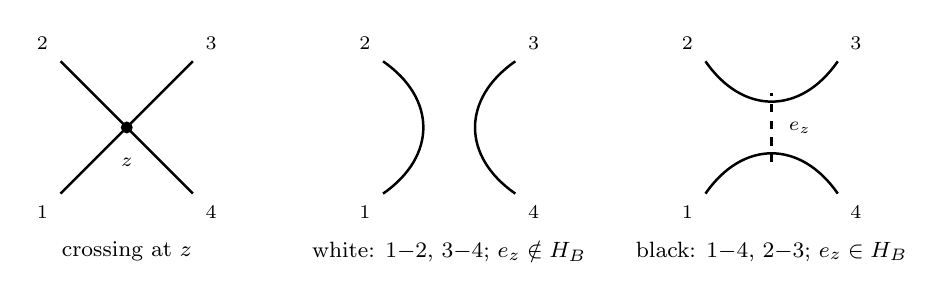
\begin{tikzpicture}[scale=1.05,line width=0.9pt]
  % --- crossing at z, with the four incident arcs labelled 1..4
  \begin{scope}
    \draw (-0.8,-0.8)--(0.8,0.8);
    \draw (-0.8,0.8)--(0.8,-0.8);
    \filldraw (0,0) circle (1.6pt);
    \node[font=\scriptsize] at (-1.02,-1.02) {$1$};
    \node[font=\scriptsize] at (-1.02, 1.02) {$2$};
    \node[font=\scriptsize] at ( 1.02, 1.02) {$3$};
    \node[font=\scriptsize] at ( 1.02,-1.02) {$4$};
    \node[font=\scriptsize] at (0,-0.42) {$z$};
    \node at (0,-1.5) {\footnotesize crossing at $z$};
  \end{scope}
  % --- white smoothing: joins 1-2 and 3-4 (e_z absent)
  \begin{scope}[xshift=3.9cm]
    \draw (-0.8,-0.8) .. controls (-0.15,-0.35) and (-0.15,0.35) .. (-0.8,0.8);
    \draw (0.8,-0.8)  .. controls (0.15,-0.35)  and (0.15,0.35)  .. (0.8,0.8);
    \node[font=\scriptsize] at (-1.02,-1.02) {$1$};
    \node[font=\scriptsize] at (-1.02, 1.02) {$2$};
    \node[font=\scriptsize] at ( 1.02, 1.02) {$3$};
    \node[font=\scriptsize] at ( 1.02,-1.02) {$4$};
    \node at (0,-1.5) {\footnotesize white: $1{-}2$, $3{-}4$; $e_z\notin H_B$};
  \end{scope}
  % --- black smoothing: joins 1-4 and 2-3; Tait edge e_z present (dashed)
  \begin{scope}[xshift=7.8cm]
    \draw (-0.8,-0.8) .. controls (-0.35,-0.15) and (0.35,-0.15) .. (0.8,-0.8);
    \draw (-0.8,0.8)  .. controls (-0.35,0.15)  and (0.35,0.15)  .. (0.8,0.8);
    \draw[dashed] (0,-0.42)--(0,0.42);
    \node[font=\scriptsize] at (0.34,0) {$e_z$};
    \node[font=\scriptsize] at (-1.02,-1.02) {$1$};
    \node[font=\scriptsize] at (-1.02, 1.02) {$2$};
    \node[font=\scriptsize] at ( 1.02, 1.02) {$3$};
    \node[font=\scriptsize] at ( 1.02,-1.02) {$4$};
    \node at (0,-1.5) {\footnotesize black: $1{-}4$, $2{-}3$; $e_z\in H_B$};
  \end{scope}
\end{tikzpicture}
\caption{Source: this work and its archived computations. The two smoothings of the frozen crossing at an ant cell $z$. The four
incident frozen arcs are labelled $1,2,3,4$. Colour selects which of the two ways they
reconnect: white joins $1{-}2$ and $3{-}4$, black joins $1{-}4$ and $2{-}3$. The black
smoothing is exactly the occupied Tait edge $e_z$ (dashed).}
\label{fig:smoothing}
\end{figure}

\begin{theorem}[Boundary-loop conjugacy]\label{thm:conjugacy}
White and black at $z$ are the two smoothings of the directed crossing at the Tait
edge $e_z$ \textup{(Figure~\ref{fig:smoothing})}. Consequently:
\begin{enumerate}[label=\textup{(\alph*)}]
\item the frozen routing loops are exactly the boundary components of a regular
neighbourhood of $H_B$, together with the untouched four-cycles;
\item the ant advances along its current frozen boundary loop and then toggles the
edge $e_z$; and
\item each step either merges two frozen loops into one or splits one into two.
\end{enumerate}
\end{theorem}

\begin{proof}
Frozen (colour-ignoring) routing is the permutation $\rho$ of directed edges of the
ant lattice sending each directed edge to the next one the ant would follow under a
fixed local turn rule; since a white cell turns right and a black cell turns left, at
each ant cell $z$ the local routing is one of the two ways of connecting the four
directed edge-ends incident to $z$ that avoids a $U$-turn. These are precisely the two
\emph{smoothings} of the $4$-valent vertex $z$ of the medial graph, and the Tait edge
$e_z$ of \eqref{eq:tait} records which diagonal pair of plaquette-corners the crossing
joins; white is one smoothing and black the other, which is (a) at the level of a
single crossing.

Now freeze a colouring $B$. Away from $H_B$ every plaquette crossing is white, and the
white smoothings assemble into the boundary circuits of a regular neighbourhood $\mathcal{N}$
of the edge subgraph $H_B$: each occupied edge $e_z$ is thickened to a band, each Tait
vertex to a disk, and the frozen routing runs along $\partial\mathcal{N}$, with the untouched
white plaquettes contributing the trivial four-cycles. (This is the standard medial/Tait
correspondence between a plane graph and the boundary of a ribbon neighbourhood.) This
gives (a) globally: the frozen loops are the components of $\partial\mathcal{N}$ plus the
untouched four-cycles. Statement (b) is immediate: the live ant sits on the current
boundary loop and, on stepping off $z$, toggles the colour of $z$, i.e.\ replaces the
smoothing at that single crossing---adding or deleting the band $e_z$ in $\mathcal{N}$.

For (c), toggling $e_z$ is the addition or deletion of one band at a $4$-valent
vertex, which is a single Dehn-twist-free band surgery on $\partial\mathcal{N}$. Locally it
reconnects the two boundary arcs passing the vertex: if the two arcs belong to the same
boundary component the surgery splits it into two, and if they belong to different
components it merges them into one. There are no other cases, giving (c).
\end{proof}

Let $E=|B|$ be the number of occupied Tait edges, $V$ the number of incident Tait
vertices, $k$ the number of nonempty components, and $\beta=E-V+k$ the cycle rank.

\begin{theorem}[Cycle-rank surgery identity]\label{thm:cyclerank}
A regular neighbourhood of $H_B$ has $k+\beta=E-V+2k$ boundary components. Writing
$\Delta C$ for the change in loop count relative to the $V$ trivial plaquette loops,
\begin{equation}\label{eq:cyclerank}
\Delta C=E-2V+2k,\qquad E+\Delta C=2\beta .
\end{equation}
Adding a bridge merges two loops and fixes $\beta$; adding a cycle edge splits a loop
and raises $\beta$ by one; removing a bridge splits a loop and fixes $\beta$;
removing a non-bridge merges two loops and lowers $\beta$ by one.
\end{theorem}

\begin{proof}
A regular neighbourhood of a plane graph with $V$ vertices, $E$ edges, and $k$
components is a compact planar surface with $k$ genus-zero pieces and Euler
characteristic $V-E$. If it has $b$ boundary circles, then $V-E=2k-b$, so
$b=E-V+2k=k+\beta$, where $\beta=E-V+k$ is the first Betti number.
Formula~\eqref{eq:cyclerank} is the difference from the $V$ trivial plaquette loops.
The four surgery cases are the standard effect on the boundary of adding or deleting
a bridge (Betti number unchanged; boundary count changes by $\mp1$) versus a cycle
edge (Betti number changes by $\pm1$; opposite merge/split), read off from
Theorem~\ref{thm:conjugacy}(c).
\end{proof}

\begin{proposition}[Advanced records are bridges]\label{prop:record}
Once a new bounding-box record lies strictly beyond the bounding box of the finite
initial support, its first visit is white, and a new east, north, west, or south
record causes the ant to turn south, east, north, or west, respectively. In the
Tait graph the corresponding edge has a previously untouched endpoint, hence is a
bridge. Therefore sufficiently advanced record creation never raises $\beta$; any
unbounded production of cycle rank occurs strictly inside already-explored territory.
\end{proposition}

\begin{proposition}[No monotone affine invariant]\label{rem:nomonotone}
No nonconstant affine combination of $(E,V,k,\beta)$ is monotone along the blank
orbit. In particular, each of $E$, $V$, $k$, and $\beta$ separately fails to be
monotone. Thus no affine combination of these four graph statistics can serve as a
monotone or Lyapunov potential along even the blank orbit.
\end{proposition}

\begin{proof}
Since $\beta=E-V+k$ identically,
$aE+bV+ck+d\beta+e=(a+d)E+(b-d)V+(c+d)k+e$, so the affine combinations of
$(E,V,k,\beta)$ are exactly those of $(E,V,k)$, and such a combination is nonconstant
precisely when $\lambda:=(a+d,\,b-d,\,c+d)\in\mathbb{R}^3$ is nonzero.

One step flips one cell, hence inserts or deletes exactly one Tait edge
$e_z=\{u,v\}$. Insertion admits exactly four cases, according to how many endpoints of
$e_z$ already meet an edge of $H_B$ and, when both do, whether they lie in a common
component; deletion reverses each. This is a complete case list, not a sample:
\begin{center}
\begin{tabular}{@{}lcc@{}}
\toprule
insertion of $e_z=\{u,v\}$ & $(\Delta E,\Delta V,\Delta k)$ & $\Delta\beta$\\
\midrule
$u,v$ both new & $(1,2,1)$ & $0$\\
exactly one of $u,v$ new & $(1,1,0)$ & $0$\\
$u,v$ both old, distinct components & $(1,0,-1)$ & $0$\\
$u,v$ both old, same component & $(1,0,0)$ & $1$\\
\bottomrule
\end{tabular}
\end{center}
Hence every increment lies in
\begin{equation}\label{eq:evkdeltas}
S_0=\pm\bigl\{(1,2,1),\,(1,1,0),\,(1,0,-1),\,(1,0,0)\bigr\},
\end{equation}
and, incidentally, $\beta$ rises exactly when the inserted edge closes a cycle and is
unchanged otherwise. All eight members of $S_0$ are realised on the blank orbit---every
state of which is compact---within the first $12{,}000$ steps, so the realised
increment set is exactly $S_0$.

Now $S_0$ is centrally symmetric by construction, since deleting an edge negates the
increment of inserting it, and $S_0$ contains the linearly independent
$(1,1,0),(1,0,-1),(1,0,0)$, so $\operatorname{span}S_0=\mathbb{R}^3$. Let
$\lambda\neq0$. Spanning gives $v\in S_0$ with $\lambda\cdot v\neq0$; replacing $v$ by
$-v\in S_0$ if necessary, $\lambda\cdot v>0$, while $\lambda\cdot(-v)<0$ and $-v$ is
realised as well. Hence $\lambda$ strictly increases at one step of the orbit and
strictly decreases at another, so it is monotone in neither direction. Equivalently,
$0$ lies in the interior of $\operatorname{conv}S_0$. The realisability witnesses are
reproduced by \path{verify_nomonotone.py} (Appendix~\ref{app:repro}).
\end{proof}

%=======================================================================
\section{Additive charges and clean translators}\label{sec:charges}
%=======================================================================

\begin{definition}\label{def:translator}
A \emph{clean finite translator with nonzero drift} is a finite state for which, for
some $N>0$ and $\drift\in\Z^2\setminus\{0\}$,
\[
B_N=B_0+\drift,\qquad p_N=p_0+\drift,\qquad q_N=q_0 .
\]
The word \emph{clean} means the entire black set translates: no stationary residue
and no newly emitted wake. This is not the ordinary highway, which grows a wake.
\end{definition}

\subsection{Laurent charges and axis alignment}
Work in the Laurent polynomial ring $\F_2[X^{\pm1},Y^{\pm1}]$, an integral domain.
Let $V_t=1$ if $q_t$ is vertical and $H_t=1-V_t$, and set
\[
A_t=\sum_{(x,y)\in B_t}X^x+V_t\,X^{x_t},\qquad
D_t=\sum_{(x,y)\in B_t}Y^y+H_t\,Y^{y_t}.
\]

\begin{proposition}\label{prop:laurent}
$A_t$ and $D_t$ are conserved. Hence a clean translator with $\drift=(a,b)$ satisfies
$A=X^aA$ and $D=Y^bD$; since $A(1)=|B|+V$ and $D(1)=|B|+H$ cannot both vanish in
$\F_2$ (because $V+H=1$), the drift coordinates $a$ and $b$ are not both nonzero.
Every clean translator is axis-aligned.
\end{proposition}

\begin{proof}
Conservation of $A_t$: on a step from a vertical cell, the toggle at column $x_t$
cancels the disappearing vertical correction $X^{x_t}$; on a step from a horizontal
cell, the post-turn motion is vertical, so $x_{t+1}=x_t$ and the toggle cancels the
newly appearing correction. Translation covariance then gives $A=X^aA$. In the
integral domain $\F_2[X^{\pm1},Y^{\pm1}]$, $a\neq0$ forces $A=0$ and $b\neq0$ forces
$D=0$; but $A(1)+D(1)=2|B|+1=1\neq0$.
\end{proof}

\begin{proposition}[Additive-charge cocycle]\label{prop:cocycle}
Let $A$ be an abelian group and $w:\Z^2\to A$. If there exist heading corrections
$F_q:\Z^2\to A$ (indexed by $q\in\Z/4\Z$) such that $\sum_{z\in B}w(z)+F_q(p)$ is
conserved under
\begin{equation}\label{eq:pot}
F_{q+1}(z+u_{q+1})-F_q(z)=-w(z)\ \ (\turnR),\qquad
F_{q-1}(z+u_{q-1})-F_q(z)=+w(z)\ \ (\turnL),
\end{equation}
then $w$ satisfies both the four-corner condition
\begin{equation}\label{eq:cocycle}
w(x{+}1,y{+}1)+w(x{+}1,y)+w(x,y{+}1)+w(x,y)=0\quad\text{in }A
\end{equation}
and $4w=0$. Conversely, if $A=\Z/4\Z$ \emph{(}so $4w=0$ holds automatically\emph{)}
and $w$ satisfies \eqref{eq:cocycle}, then such $F_q$ exist. Over $\F_2$ the solutions
of \eqref{eq:cocycle} are exactly $w(x,y)=\alpha(x)+\beta(y)$.
\end{proposition}

\begin{proof}
\emph{Necessity.} Eliminating the four $F_q$ from \eqref{eq:pot} around a unit
plaquette gives the four-corner condition \eqref{eq:cocycle}. For $4w=0$, combine the
four relations at a single cell $z$: the $\turnR$-at-$S$ and $\turnL$-at-$N$ relations
both express $F_W(z+u_W)$, forcing $F_S(z)=F_N(z)+2w(z)$, while the $\turnL$-at-$S$ and
$\turnR$-at-$N$ relations force $F_S(z)=F_N(z)-2w(z)$; hence $4w(z)=0$. Thus
$w(x,y)=(-1)^{x+y}$ over $A=\Z$ satisfies \eqref{eq:cocycle} but admits no such $F_q$,
since $4w\neq0$.

\emph{Sufficiency for $A=\Z/4\Z$.} Composing pairs of relations in \eqref{eq:pot}
expresses $F_N$ by its diagonal increments
\begin{equation}\label{eq:Fdiag}
\begin{aligned}
F_N(x{+}1,y{+}1)-F_N(x,y)&=-w(x,y)+w(x{+}1,y),\\
F_N(x{+}1,y{-}1)-F_N(x,y)&=w(x,y{-}1)-w(x{+}1,y{-}1).
\end{aligned}
\end{equation}
which define $F_N$ on each of the two $x{+}y$-parity sublattices by integration from a
basepoint. Modulo four, the circulation of \eqref{eq:Fdiag} around the elementary
diamond $(x,y)\to(x{+}1,y{+}1)\to(x{+}2,y)\to(x{+}1,y{-}1)\to(x,y)$ equals the negative
of the sum of the four-corner expressions \eqref{eq:cocycle} based at $(x,y{-}1)$ and
$(x{+}1,y{-}1)$ (the two differ by $4\,[w(x{+}1,y)+w(x{+}1,y{-}1)]\equiv0$); hence it
vanishes by \eqref{eq:cocycle}, so the integration is path-independent and $F_N$ is
well defined. Now set $F_S=F_N-2w$ and define $F_E,F_W$ from $F_N$ by \eqref{eq:pot}.
Substituting these definitions back into the four $\turnR/\turnL$ relations verifies
each case in turn; the only possible ambiguity is between the two ways of reaching
$F_S$---via the $\turnR$-at-$S$/$\turnL$-at-$N$ pair, which gives $F_N+2w$, and via the
$\turnL$-at-$S$/$\turnR$-at-$N$ pair, which gives $F_N-2w$---and their discrepancy is
exactly $4w$, which vanishes. Hence all four $F_q$ are consistent. Over $\F_2$ the
solution space of \eqref{eq:cocycle} is the separable weights $\alpha(x)+\beta(y)$.
\end{proof}

\subsection{The strand decomposition}
Let $\growth=\#\turnR-\#\turnL$ over one period. Lemma~\ref{lem:invariant} gives
$\growth\equiv0\pmod4$, and $\growth\ge0$ because $\growth$ equals the number of
\emph{odd} stabilised translation classes of Theorem~\ref{thm:criterion} (a class is
odd iff its stabilised word has odd length, contributing one net black cell per
period). We record the endpoint structure used in Section~\ref{sec:residue}.

\begin{proposition}[Canonical endpoint decomposition]\label{prop:decomp}
The one-period signed toggle pattern $D:\Z^2\to\Z$ (with $D(z)=\#\{\turnR\text{ at }z\}-\#\{\turnL\text{ at }z\}$ over one period) decomposes as
\begin{equation}\label{eq:decomp}
D=S+(T_\drift-1)A,\qquad S=\sum_{i=1}^{\growth}\delta_{c_i},
\end{equation}
where $(T_\drift A)(z)=A(z-\drift)$, $A$ is a finitely supported \emph{moving widget},
and $c_1,\dots,c_\growth\in\Z^2$ are the bases of the $\growth$ growing strands, one
per odd stabilised class. For the standard word $\growth=12$ and $|B_n|=11+12n$ at
period boundaries.
\end{proposition}

\begin{proof}
$D$ is finitely supported (only finitely many cells are visited in one period).
Partition the support into translation classes under $z\mapsto z+\drift$; there are
finitely many nonempty classes. Fix a class with base point $c$ and write
$f(n)=D(c+n\drift)\in\Z$, a finitely supported function $\Z\to\Z$. Put $s=\sum_n f(n)$
and $h=f-s\,\delta_0$, so $\sum_n h(n)=0$. With the shift $(Ta)(n)=a(n-1)$, set
\[
a(n)=\sum_{m>n}h(m).
\]
Then $a(n-1)-a(n)=h(n)$, i.e.\ $(T-1)a=h$, so
\[
f=s\,\delta_0+(T-1)a,
\]
and $a$ is finitely supported: $a(n)=0$ for $n$ beyond the support of $f$ on the
right, and $a(n)=\sum_m h(m)=0$ for $n$ far to the left (this is exactly where
$\sum h=0$ is needed). Summing over all classes gives \eqref{eq:decomp} with $A$ the
(finite) sum of the class antiderivatives and $S=\sum_{\text{classes}}s_c\,\delta_{c}$. It remains to
identify $\sum_n f$ for a class. Over one period the cells of a class are visited in
level order, and the alternating-visit rule (Proposition~\ref{prop:alt}) makes the
per-class toggle total equal to $+1$ when the class's stabilised word has odd length
(an ``odd class'') and $0$ when it has even length; thus $\sum_n f\in\{0,1\}$ and
$S$ is a sum of $\growth$ unit masses, one per odd class, where
$\growth=\#\{\text{odd classes}\}=\#\turnR-\#\turnL$ (the last equality because both
count the net black cells created per period). The standard-word figures follow from
$|B_0|=11$ and $|B_{n+1}|-|B_n|=\growth=12$.
\end{proof}

\begin{corollary}\label{cor:sep}
If $\growth=0$ then a finite stationary set can be deleted to leave a clean finite
translator with drift $\drift$.
\end{corollary}

\begin{proof}
Here $S=0$, so $D=(T_\drift-1)A$. Let $b_n:\Z^2\to\{0,1\}$ be the indicator of $B_n$
at the $n$-th period boundary. Since each cell is toggled a net $D(z)\in\{-1,0,+1\}$
per period (Proposition~\ref{prop:alt}) and the period-$k$ toggle pattern is
$T_{k\drift}D$ by translation covariance,
\[
b_n=b_0+\sum_{k=0}^{n-1}T_{k\drift}D
   =b_0+\sum_{k=0}^{n-1}T_{k\drift}(T_\drift-1)A
   =b_0+(T_{n\drift}-1)A=R+T_{n\drift}A,\qquad R:=b_0-A .
\]
Both $R$ and $A$ are finitely supported, so for $n$ large the supports of $R$ and
$T_{n\drift}A$ are disjoint; since $b_n$ is $\{0,1\}$-valued, $R$ and $A$ are then
$\{0,1\}$-valued and $B_n=R\sqcup(A+n\drift)$. Because the trace is periodic with
nonzero drift, each cell is visited finitely often, so at a sufficiently late period
boundary the ant never again visits the finite set $R$. Deleting $R$ there changes no
future turn and leaves a state whose black set is $A+n\drift$, translating exactly by
$\drift$ each period: a clean finite translator.
\end{proof}

Sections~\ref{sec:evenwinding} and~\ref{sec:residue} prove, by two independent
routes, that no such clean translator exists; hence $\growth\neq0$.

%=======================================================================
\section{The even-winding theorem}\label{sec:evenwinding}
%=======================================================================

This section proves that no clean translator exists, via a cylinder homology
argument. Lemma~\ref{lem:localparity} supplies the local parity identity
relating the turn count at a cell to its horizontal edge parity.

\begin{theorem}[Even-winding theorem]\label{thm:evenwinding}
No finite-support clean translator with nonzero drift exists.
\end{theorem}

For the remainder of the section fix a hypothetical clean translator. Its drift is
axis-aligned by Proposition~\ref{prop:laurent}. A clean translator has $\growth=0$, so
its period $N=\#\turnR+\#\turnL=2\#\turnR$ is even; since each step changes $x+y$
modulo $2$, the total displacement satisfies $a+b\equiv N\equiv0\pmod2$, so the
nonzero drift coordinate is even. After a quarter-turn rotation write $\drift=(L,0)$
with $L>0$ even---all that the argument below requires. Writing $B_j,p_j$ for the black
set and ant position at phase $j$ of one period, reversibility and translation
covariance give, for all $n\in\Z$,
\[
B_{nN+j}=B_j+n\drift,\qquad p_{nN+j}=p_j+n\drift .
\]
Quotient the bi-infinite trace by translation through $\drift$ to obtain a closed
walk on the cylinder $C_L=(\Z/L\Z)\times\Z$; because $L$ is even the HV type of
Proposition~\ref{prop:hv} descends to $C_L$. For an undirected cylinder edge, its
\emph{multiplicity} is the number of traversals by the projected one-period walk.

\begin{lemma}[Visit count]\label{lem:visit}
Every vertex $v$ of $C_L$ is visited $n_v=2k_v$ times in one quotient period, with
exactly $k_v$ turns $\turnR$ and $k_v$ turns $\turnL$.
\end{lemma}

\begin{proof}
Let $z$ be a physical representative of $v$. Each phase $j$ with $p_j\in v+\Z\drift$
has a unique level $m_j$ with $p_j=z+m_j\drift$, and phase $j$ in period $-m_j$ visits
$z$; conversely every visit to $z$ over the bi-infinite orbit arises once this way.
Hence the visits to $v$ in one quotient period biject with the visits to $z$ over the
translated bi-infinite orbit. At phase $nN+j$ the black pattern is the finite translate
$B_j+n\drift$, so $z$ is white for all sufficiently early and all sufficiently
late times. Its turn sequence therefore alternates, begins with $\turnR$, ends with
$\turnL$, and contains equally many of each.
\end{proof}

At a vertex $v$ let $H_{v,-},H_{v,+}$ be the multiplicities of the west and east
horizontal edges and $V_{v,-},V_{v,+}$ those of the south and north vertical edges.
By Proposition~\ref{prop:hv} one pair carries all arrivals and the other all
departures, and each visit is one arrival plus one departure, so
\begin{equation}\label{eq:balance}
H_{v,-}+H_{v,+}=V_{v,-}+V_{v,+}=2k_v .
\end{equation}

\begin{lemma}[Edge parities]\label{lem:edgeparity}
The horizontal-edge multiplicity has a constant parity $h_y\in\F_2$ along each row
$y$. Every vertical-edge multiplicity is even; write $V_e=2G_e$ with $G_e\in\Z_{\ge0}$.
\end{lemma}

\begin{proof}
Reducing the horizontal half of \eqref{eq:balance} modulo $2$ gives
$H_{v,-}\equiv H_{v,+}$, so consecutive horizontal edges in a row share parity;
call it $h_y$. The vertical half gives $V_{v,-}\equiv V_{v,+}$, so vertical parity is
constant up each column. The projected walk has finite vertical support, so a
vertical edge far enough below or above it has multiplicity $0$; constancy then forces
every vertical multiplicity even.
\end{proof}

\begin{lemma}[Local parity]\label{lem:localparity}
At every vertex $v=(x,y)$ of $C_L$, $\;k_v\equiv h_y\pmod2$.
\end{lemma}

\begin{proof}
Suppose $v$ is vertical (the horizontal case is the $90^\circ$ rotation). By
Proposition~\ref{prop:hv} the ant arrives at $v$ along a vertical edge---from the
south moving north, or from the north moving south---and departs along a horizontal
edge. Record each visit by (arrival direction, turn). Using
$u_{q+\varepsilon}$ from \eqref{eq:step}: an arrival from the south ($\turnR$) departs
east, from the south ($\turnL$) departs west, from the north ($\turnR$) departs west,
from the north ($\turnL$) departs east. Let $a_{\turnR},a_{\turnL}$ count arrivals
from the south with the two turns and $b_{\turnR},b_{\turnL}$ those from the north.
Because the east edge is only ever traversed \emph{out} of $v$ (its other endpoint is
horizontal, hence cannot depart along it), its multiplicity equals the number of east
departures:
\[
H_{v,+}=a_{\turnR}+b_{\turnL}.
\]
The north edge is only ever traversed \emph{into} $v$, with multiplicity
$V_{v,+}=b_{\turnR}+b_{\turnL}$. The total turn count is $k_v=a_{\turnR}+b_{\turnR}$.
Hence
\[
H_{v,+}-k_v=(a_{\turnR}+b_{\turnL})-(a_{\turnR}+b_{\turnR})=b_{\turnL}-b_{\turnR}
\equiv b_{\turnL}+b_{\turnR}=V_{v,+}\pmod2 .
\]
By Lemma~\ref{lem:edgeparity}, $H_{v,+}$ has parity $h_y$ and $V_{v,+}$ is even; therefore
$h_y\equiv k_v\pmod2$.
\end{proof}

\begin{proof}[Proof of Theorem~\ref{thm:evenwinding}]
Halving the vertical half of \eqref{eq:balance} and using $V_e=2G_e$ gives the exact
identity $k_{x,y}=G_{x,y-1/2}+G_{x,y+1/2}$, where $G_{x,y\pm1/2}$ denote the halved
multiplicities of the vertical edges below and above $v$. Fix a column $x$ and sum
Lemma~\ref{lem:localparity} over all rows:
\begin{equation}\label{eq:telescope}
\sum_y h_y\ \equiv\ \sum_y k_{x,y}\ =\ \sum_y\bigl(G_{x,y-1/2}+G_{x,y+1/2}\bigr)\ \equiv\ 0\pmod2,
\end{equation}
because each interior half-edge $G$ appears exactly twice and the two exterior terms
vanish by finite vertical support.

Now cut $C_L$ along a vertical seam between two adjacent columns. The algebraic
winding number $w$ of the projected closed walk is the signed number of seam
crossings; there is exactly one horizontal seam edge in each row $y$, of multiplicity
$\equiv h_y\pmod2$, and signs vanish modulo $2$, so
\[
w\equiv\sum_y h_y\equiv0\pmod2
\]
by \eqref{eq:telescope}. On the other hand the lift of the closed walk runs from $p$
to $p+(L,0)$, so it winds exactly once around $C_L$: $w=1$. This contradiction proves
the theorem for drift $(L,0)$; quarter-turn rotations (including a half-turn) cover the
remaining axis-aligned drifts.
\end{proof}

\begin{corollary}[Growth is a positive multiple of four]\label{cor:growth4}
Every finite-support periodic highway has net black growth
\begin{equation}\label{eq:growth4}
\growth\in4\Z_{>0}.
\end{equation}
In particular every finite-support periodic highway builds a nonempty wake.
\end{corollary}

\begin{proof}
Zero drift confines the ant to the finitely many positions of one period, excluded by
Theorem~\ref{thm:unbounded}. Negative growth cannot recur forever since $b_t\ge0$. A
heading-resetting period has $\growth\equiv0\pmod4$ (Lemma~\ref{lem:invariant}). If
$\growth=0$ then by Corollary~\ref{cor:sep} the state reduces, after deleting a finite
stationary set never revisited, to a clean finite translator with nonzero drift,
contradicting Theorem~\ref{thm:evenwinding}. Hence $\growth>0$, and
$\growth\in4\Z_{>0}$.
\end{proof}

The standard highway has $\growth=12$, consistent with \eqref{eq:growth4}. The
telescope \eqref{eq:telescope} is the finite algebraic core machine-checked in Lean
(Appendix~\ref{app:lean}).

%=======================================================================
\section{The signed mod-four wake-residue theorem}\label{sec:residue}
%=======================================================================

We now give a second, independent proof that no zero-growth periodic highway exists,
which additionally pins the arithmetic relation between growth and drift. Recall the
strand bases $c_1,\dots,c_\growth$ of Proposition~\ref{prop:decomp}.

\begin{theorem}[Signed mod-four wake-residue identity]\label{thm:residue}
Let a finite-support repeating trace have restored heading, nonzero drift
$\drift=(a,b)$, growth $\growth$, and decomposition \eqref{eq:decomp}. Then:
\begin{enumerate}[label=\textup{(\roman*)}]
\item if $a\neq0$, then for every residue $r\in\Z/|a|\Z$,
\begin{equation}\label{eq:res-a}
\sum_{i:\;c_{i,x}\equiv r\ (\mathrm{mod}\ |a|)}\che(c_i)\ \equiv\ 2\pmod4;
\end{equation}
\item if $b\neq0$, the analogous sum over each residue of $c_{i,y}$ modulo $|b|$ is
$\equiv2\pmod4$;
\item if $a=0$, the signed sum $\sum_{i:\,c_{i,x}=x_0}\che(c_i)$ over each exact
column $x_0$ is $\equiv0\pmod4$; symmetrically for exact rows when $b=0$.
\end{enumerate}
\end{theorem}

The proof rests on a monodromy computation for the potentials of
Proposition~\ref{prop:cocycle}.

\begin{lemma}[Diagonal increment and vertical periodicity]\label{lem:diag}
Fix $a\neq0$ and any $\alpha:\Z/|a|\Z\to\Z/4\Z$, and set $w(x,y)=\che(x,y)\,\alpha(x)$,
a weight valued in $\Z/4\Z$. Then $w$ satisfies the four-corner condition
\eqref{eq:cocycle} in $A=\Z/4\Z$, so potentials $F_q$ as in
\eqref{eq:pot} exist, and
\begin{equation}\label{eq:diag}
F_N(x{+}1,y{+}1)-F_N(x,y)=-\che(x,y)\bigl(\alpha(x)+\alpha(x{+}1)\bigr),
\end{equation}
while $F_N$ is $2$-periodic in $y$.
\end{lemma}

\begin{proof}
Since $\che(x{+}1,y{+}1)=\che(x,y)$ and $\che(x{+}1,y)=\che(x,y{+}1)=-\che(x,y)$, the
four-corner sum \eqref{eq:cocycle} telescopes to
$\che(x,y)[\alpha(x{+}1)-\alpha(x{+}1)-\alpha(x)+\alpha(x)]=0$;
so $F_q$ exist by Proposition~\ref{prop:cocycle}. Compose the $\turnR$ step at $(x,y)$ heading $N$ (giving
$F_E(x{+}1,y)-F_N(x,y)=-w(x,y)$) with the $\turnL$ step at $(x{+}1,y)$ heading $E$
(giving $F_N(x{+}1,y{+}1)-F_E(x{+}1,y)=+w(x{+}1,y)$). Adding,
\[
F_N(x{+}1,y{+}1)-F_N(x,y)=-w(x,y)+w(x{+}1,y)=-\che(x,y)\alpha(x)-\che(x,y)\alpha(x{+}1),
\]
which is \eqref{eq:diag}. The relation $F_S=F_N-2w$ (from composing the two vertical
steps) gives the same increment along $(1,-1)$; combining the $(1,1)$ and $(1,-1)$
increments over a closed square shows $F_N(x,y{+}2)=F_N(x,y)$.
\end{proof}

\begin{proof}[Proof of Theorem~\ref{thm:residue}]
Fix $a\neq0$, $\alpha$, and $w$ as in Lemma~\ref{lem:diag}. Restored heading gives
$\growth\equiv0\pmod4$, so the period is even and $a+b$ is even; hence translation by
$\drift$ preserves $\che$, and $w(z+\drift)=w(z)$. Let $\varepsilon=\operatorname{sgn}(a)$,
and set $\sigma=\operatorname{sgn}(b)$ if $b\neq0$ and $\sigma=1$ if $b=0$. Move from
$z$ to $z+\drift$ by $|a|$ diagonal steps of vector $(\varepsilon,\sigma)$, followed by
the vertical displacement $(0,\,b-\sigma|a|)$, which is even because $a+b$ is even. The
uniform diagonal increment of $F_N$ (read off from \eqref{eq:diag} for
$\varepsilon=+1$ and from its reverse for $\varepsilon=-1$) is
\begin{equation}\label{eq:uniform}
F_N(x+\varepsilon,y+\sigma)-F_N(x,y)=-\varepsilon\,\che(x,y)\bigl(\alpha(x)+\alpha(x+\varepsilon)\bigr),
\end{equation}
and $\che$ is constant along the path because $\varepsilon+\sigma$ is even; the
vertical part contributes nothing by the $2$-periodicity of $F_N$ in $y$. As $x$ runs
once through $\Z/|a|\Z$ each $\alpha(r)$ appears twice, so the increments telescope to
$-2\varepsilon\,\che(z)\sum_{r}\alpha(r)$, giving the monodromy
\begin{equation}\label{eq:monodromy}
F_N(z+\drift)-F_N(z)\ \equiv\ 2\sum_{r\in\Z/|a|\Z}\alpha(r)\pmod4
\end{equation}
(since $-2\varepsilon\che(z)\equiv2\pmod4$ for either sign of $a$). The three other headings satisfy the same relation: $F_S=F_N-2w$
and $F_E,F_W$ differ from $F_N$ by single applications of \eqref{eq:pot}, all of which
are themselves $\drift$-periodic because $w$ is; so \eqref{eq:monodromy} holds with
$F_q$ in place of $F_N$ for every $q$, and for either sign of $a$.

Charge conservation of $\sum_{z\in B}w(z)+F_q(p)$ over one period gives
\begin{equation}\label{eq:conservation}
\sum_{z}D(z)\,w(z)+F_q(p+\drift)-F_q(p)=0,
\end{equation}
where $D$ is the signed toggle pattern of Proposition~\ref{prop:decomp}. Because $w$
is $\drift$-periodic and $(T_\drift A)(z)=A(z-\drift)$, the widget terms cancel:
$\sum_z(T_\drift A)(z)w(z)=\sum_zA(z)w(z)$. Substituting $D=S+(T_\drift-1)A$ and the
monodromy \eqref{eq:monodromy} into \eqref{eq:conservation},
\begin{equation}\label{eq:reduced}
\sum_{i=1}^{\growth}\che(c_i)\,\alpha(c_{i,x})+2\sum_{r\in\Z/|a|\Z}\alpha(r)\ \equiv\ 0\pmod4 .
\end{equation}
Taking $\alpha=\mathbf 1_{\{r\}}$ turns \eqref{eq:reduced} into
$\sum_{i:\,c_{i,x}\equiv r}\che(c_i)+2\equiv0$, i.e.\ \eqref{eq:res-a}, using
$-2\equiv2$. Rotating by $90^\circ$ gives (ii). For $a=0$, take a finitely supported
exact-column $\alpha:\Z\to\Z/4\Z$; then $b$ is even, $w$ is $\drift$-periodic, the
vertical $2$-periodicity makes the monodromy vanish, and exact-column indicators give
(iii).
\end{proof}

\begin{corollary}[Strand-density bound]\label{cor:P16}
Every finite-support repeating trace with drift $\drift=(a,b)$ has
\begin{equation}\label{eq:P16}
\growth\ \ge\ 2\max(|a|,|b|).
\end{equation}
In particular $\growth=0$ is impossible---an independent proof of
Theorem~\ref{thm:evenwinding}. If a residue fiber contains exactly two strand bases,
they share checkerboard parity; for $\drift=(\pm2,\pm2)$ and $\growth=4$ the
$2\times2$ residue-count matrix is $\left[\begin{smallmatrix}2&0\\0&2\end{smallmatrix}\right]$
or $\left[\begin{smallmatrix}0&2\\2&0\end{smallmatrix}\right]$.
\end{corollary}

\begin{proof}
A sum of $m$ signs $\pm1$ congruent to $2\pmod4$ is nonzero, with $m$ positive and
even. Hence each of the $|a|$ residue classes modulo $|a|$ contains at least two
strand bases, giving $\growth\ge2|a|$; symmetrically $\growth\ge2|b|$. If $\growth=0$
some class is empty while $\drift\neq0$, contradicting \eqref{eq:res-a}. A two-element
fiber has $\che$-sum $\pm2$, forcing equal signs. When
$\drift=(\pm2,\pm2)$ and $\growth=4$, every row and column of the $2\times2$ residue
matrix therefore has sum $2$. Equal checkerboard signs in either fixed-$x$ row force
its two bases into the same $y$-parity column, ruling out the matrix with all entries
$1$; the only possibilities are the two matrices displayed in the statement.
\end{proof}

\begin{remark}
The bound \eqref{eq:P16} is a genuine lower bound but is not claimed to be attained by
a chronological highway: the standard highway has $\growth=12$ against
$2\max(2,2)=4$. Determining which residue profiles can be realised by a single ant
tour is part of the chronology problem left open in Section~\ref{sec:gap}.
\end{remark}

\subsection{An all-period axis growth-four exclusion}

The next result is the first use here of the \emph{order} of all visits in a
translation class, rather than only their totals.  For a phase $i$ in a trace with
$\drift=(2,0)$, write $p_i=(x_i,y_i)$ and
\[
\ell_i=\frac{x_i-(x_i\bmod2)}2,
\qquad \tau_i=i-N\ell_i.
\]
Within a class $(x_i\bmod2,y_i)$, increasing $\tau_i$ is precisely the stabilised
order of Remark~\ref{rem:onesort}: decreasing $x_i$, then increasing phase.  Denote
the zero-based rank in that order by $r_i$.

\begin{theorem}[Axis growth four is impossible]\label{thm:axisg4}
No finite-support periodic highway with growth $\growth=4$ has axis drift.
\end{theorem}

\begin{proof}
The density bound and checkerboard parity reduce a nonzero axis drift at growth four,
after a quarter-turn rotation, to $\drift=(2,0)$.  Translate $p_0$ to the origin and
cyclically choose a phase whose arrival heading is vertical.  Put $N=2M$ and group
the moves into $M$ horizontal--vertical pairs.  The horizontal displacement is two,
so $M$ is even.

We first prove a kinematic rank identity requiring neither the
periodic-realisability criterion nor growth four.  Set
\begin{equation}\label{eq:rankK}
K=\sum_{i:\,w_i=\turnL}r_i\pmod2.
\end{equation}
For every heading-reset single tour from the origin to $(2,0)$,
\begin{equation}\label{eq:rankparity}
K\equiv 1+\frac M2=1+\frac N4\pmod2.
\end{equation}

To prove \eqref{eq:rankparity}, the two-column quotient has on each used row $y$ a
vertical-arrival class $Q_y$ and a horizontal-arrival class $C_y$.  At any one of
these classes, list its $n$ occurrences in stable-rank order and let
$\alpha_r,\beta_r\in\{0,1\}$ indicate respectively the positive incoming and
outgoing ports.  Positive means north/east at $Q_y$ and east/north at $C_y$.  If
$A=\sum_r\alpha_r$ and $I(\alpha)$ is the parity of pairs $r<s$ with
$\alpha_r=1$, $\alpha_s=0$, then
\begin{equation}\label{eq:binaryinv}
I(\alpha)\equiv A(n-1)+\sum_r r\alpha_r+\binom A2\pmod2.
\end{equation}
At $Q_y$ a left turn means $\alpha_r\ne\beta_r$, whereas at $C_y$ it means
$\alpha_r=\beta_r$.  Applying \eqref{eq:binaryinv} to both port lists and summing over
all quotient classes, every binomial term is the same positive directed-edge count
at its source and target, hence occurs twice and cancels.

Write $h_y$ for the number of horizontal segments on row $y$, $e_y$ for the
east-going ones, and $n_y$ for north segments from row $y$ to $y+1$.  Closed
vertical flow gives $h_y=n_{y-1}+n_y$.  The remaining linear terms at $Q_y$ and
$C_y$ have positive-port counts $(n_{y-1},e_y)$ and $(e_y,n_y)$, so together they
are $h_y(h_y-1)=0$ modulo two.  Consequently
\begin{equation}\label{eq:Klocal}
K\equiv\sum_v\bigl(I(\alpha_v)+I(\beta_v)\bigr)
       +\sum_y\binom{h_y}{2}\pmod2.
\end{equation}

It remains to evaluate the first sum.  Order the quotient vertices as
$(Q_y,C_y)$ by increasing $y$, and put the negative port before the positive port.
Sorting occurrences by outgoing port, following one ant edge, and unsorting by
incoming port factors the phase-successor permutation.  Each directed edge block
preserves stable order: along a fixed quotient edge the successor changes $\tau_i$
by a constant.  This includes the cyclic edge from phase $N-1$ to phase zero, where
$p_N=p_0+(2,0)$ supplies the extra level (so on that edge
$\tau_0-\tau_{N-1}=1$ after using the translated endpoint).  The successor itself is one even-length
cycle, hence has sign parity one.

Let $E$ be the parity of the remaining edge-block permutation.  Its outgoing blocks
on row $y$ are $[W_y,E_y,S_y,N_y]$, while its incoming blocks are
$[S_{y+1},N_{y-1},W_y,E_y]$.  The only reversed block pairs are a horizontal block
$H_y$ against $S_y,S_{y+1}$ and $N_y$ against $S_{y+1},S_{y+2}$.  If $s_y$ counts
south segments from row $y$, then
\[
E\equiv\sum_y h_y(s_y+s_{y+1})+n_y(s_{y+1}+s_{y+2})\pmod2.
\]
Cut balance gives $s_{y+1}=n_y$ and $h_y=n_{y-1}+n_y$.  Since
$M=\sum_yh_y=2\sum_yn_y$,
\[
E\equiv\sum_yn_y+\sum_yn_yn_{y+1},\qquad
\sum_y\binom{h_y}{2}\equiv\sum_yn_yn_{y+1}\pmod2.
\]
The permutation factorisation says
$\sum_v(I(\alpha_v)+I(\beta_v))+E\equiv1$.  Substitution in
\eqref{eq:Klocal} proves \eqref{eq:rankparity}.

We now restore the highway hypotheses.  Theorem~\ref{thm:residue} and
$\growth=4$ put exactly two odd strand classes in each $x$-residue.  A fixed row
contains at most one odd class of either $x$-residue, hence at most two bases.  The
exact-row congruence for the zero $y$-component therefore forces every occupied row's
signed sum to be literally zero.  Each such row contains the opposite-checker pair;
there are exactly two rows.  Thus exactly $A_0=2$
odd classes lie on even checkerboard cells.

Let $u_j\in\{\pm1\}$ be the horizontal step and $v_j\in\{\pm1\}$ the incoming
vertical direction of pair $j$.  The even-phase turn sign ($\turnR=+1$,
$\turnL=-1$) is $u_jv_j$.  Theorem~\ref{thm:criterion} makes its sum equal to
$A_0$: every stabilised class has excess one if odd and zero if even.  Heading reset
and endpoint $(2,0)$ make the cyclic incoming vertical signs a reindexing of the
outgoing vertical steps, so $\sum_jv_j=0$; hence
\[
M+2+0+A_0
=\sum_j(1+u_j+v_j+u_jv_j)
=\sum_j(1+u_j)(1+v_j)\equiv0\pmod4.
\]
Hence $M\equiv0\pmod4$, or $N\equiv0\pmod8$.  Theorem~\ref{thm:criterion} also makes every left turn occur
at odd stable rank, so
\[
K\equiv\#\turnL=\frac{N-4}{2}\equiv0\pmod2.
\]
But \eqref{eq:rankparity} gives $K\equiv1$, a contradiction.  Quarter-turn rotations
cover every axis direction.
\end{proof}

\subsection{An all-period even-diagonal growth-four exclusion}

The same rank-sign method has a two-lane form.  Here \emph{even-diagonal} means
that both drift components are nonzero and even.  At growth four,
Corollary~\ref{cor:P16} forces both absolute values to be two, so a quarter-turn
normalises the drift to $\drift=(2,-2)$.  Put $t=x+y$ and $r=x\bmod2$, and choose phase zero to be a
vertical-arrival event at the origin.  Thus vertical-arrival quotient classes $Q$
have even $t$, while horizontal-arrival classes $C$ have odd $t$.  For an event at
$(x,y)$ define
\[
 \ell=\frac{x-r}{2},\qquad \tau=i-N\ell .
\]
Increasing $\tau$ is again the stabilised order within the translation class
$(t,r)$; write $r_i$ for the zero-based rank of phase $i$ and retain the definition
$K=\sum_{w_i=\turnL}r_i\pmod2$ from \eqref{eq:rankK}.

\begin{theorem}[Even-diagonal growth four is impossible]\label{thm:evendiagg4}
No finite-support periodic highway with growth $\growth=4$ has even-diagonal drift.
\end{theorem}

\begin{proof}
At a quotient class $v$ of multiplicity $m_v$, list occurrences in stabilised
order and use the same positive incoming and outgoing bits $\alpha,
\beta$ as in the proof of Theorem~\ref{thm:axisg4}: north/east at $Q$, and
east/north at $C$.  Put $p_v=\sum\alpha+\sum\beta\pmod2$, and let
$D_v=\#\turnR-\#\turnL$ at $v$.  Theorem~\ref{thm:criterion} gives
$D_v\in\{0,1\}$.

Apply \eqref{eq:binaryinv} to the two port lists.  At $Q$ a left turn means that
the bits differ, whereas at $C$ it means that they agree.  Since
\[
 D_Q\equiv m_v-2p_v\pmod4,
 \qquad D_C\equiv2p_v-m_v\pmod4,
\]
the non-inversion correction to the local left-rank sum is
\begin{equation}\label{eq:diaglocal}
 p_v(D_v+1)\quad\hbox{at $Q$},
 \qquad D_v(p_v+1)\quad\hbox{at $C$}.
\end{equation}
Here, as before, every positive-edge binomial occurs at both ends of its directed
edge and cancels in the global sum.

Order directed edge blocks lexicographically by $(t,r,\text{port})$, with the
negative port first, and let $E$ be the parity of the induced edge-block
permutation.  Occurrences within any one directed block preserve stabilised order:
successor changes $\tau$ by a constant fixed by that quotient edge, including at
the cyclic seam after using $p_N=p_0+(2,-2)$.  The phase successor is one even
cycle, so the same port-sorting factorisation as above gives
\begin{equation}\label{eq:diagK}
 K\equiv1+E+L\pmod2,
\end{equation}
where $L$ is the sum of the corrections in \eqref{eq:diaglocal}.

We evaluate $E+L$ by a two-lane lemma.  Write $w_{t,r},e_{t,r},s_{t,r},n_{t,r}$
for the parities of the four directed block multiplicities.  Flow at even $Q$
layers $t$ and odd $C$ layers $j$ is
\begin{align}
 w_{t,r}+e_{t,r}&=s_{t+1,r}+n_{t-1,r},\label{eq:diagflowQ}\\
 s_{j,r}+n_{j,r}&=w_{j+1,1-r}+e_{j-1,1-r}.\label{eq:diagflowC}
\end{align}
Let $O=\{v:D_v=1\}$ and let $o_r$ count its vertices in lane $r$.
Suppose first that $O$ lies on the $C$ layers.  Every $Q$ multiplicity is even, so
$w_{t,r}=e_{t,r}=:a_{t,r}$ and $s_{j,r}=n_{j-2,r}$.  Equations
\eqref{eq:diagflowQ}--\eqref{eq:diagflowC} imply
\[
 a_{t,r}+n_{t-1,1-r}=a_{t+2,r}+n_{t+1,1-r}.
\]
The sequences have finite support, hence this constant is zero and
$a_{t,r}=n_{t-1,1-r}$.  It follows that $p_v=D_v$ at every $C$ vertex, while the
two $Q$ values of $p_v$ on a fixed layer sum to zero.  Thus $L=0$.

For each $n_{j,r}=1$, the odd directed blocks form the four-edge gadget
\[
 G^C_{j,r}=\{N_{j,r},S_{j+2,r},W_{j+1,1-r},E_{j+1,1-r}\}.
\]
Its source-block order is $[N,W,E,S]$ and its target-block order is
$[W,S,N,E]$, so it has odd sign.  Comparing the eight source and target keys of
two distinct gadgets shows that their cross-inversion parity is one exactly when
they occupy the same lane and their layer indices differ by two; it is zero for
opposite lanes and for larger separation.  Therefore
\begin{equation}\label{eq:diagedgesign}
 E\equiv\sum_{j,r}n_{j,r}+\sum_{j,r}n_{j,r}n_{j+2,r}\pmod2.
\end{equation}
For a fixed lane this is the parity of the number $k_r$ of runs of ones in the
finite binary sequence $n_{j,r}$.  Its boundary is
$D_{j,r}=n_{j-2,r}+n_{j,r}$, so $o_r=2k_r$ and
\[
 E+L\equiv\sum_r k_r\equiv\sum_r\binom{o_r}{2}\pmod2.
\]

If instead $O$ lies on the $Q$ layers, every $C$ multiplicity is even.  Then
$s_{j,r}=n_{j,r}=:b_{j,r}$, $w_{t,r}=e_{t-2,r}$, and finite support in
\eqref{eq:diagflowQ}--\eqref{eq:diagflowC} gives $e_{t,r}=b_{t+1,r}$.
Now $p_v=D_v$ at $Q$, all local corrections vanish, and the gadgets are
\[
 G^Q_{j,r}=\{S_{j,r},N_{j,r},E_{j-1,r},W_{j+1,r}\}.
\]
Their source and target orders are $[E,S,N,W]$ and $[S,W,E,N]$; the identical
self- and cross-inversion table proves the same formula.  We have therefore shown,
whenever all odd classes have one checkerboard parity, that
\begin{equation}\label{eq:diagladder}
 E+L\equiv\sum_{r=0}^1\binom{o_r}{2}\pmod2.
\end{equation}

For $\growth=4$, Corollary~\ref{cor:P16} gives one of the two doubled perfect
matching residue matrices, indexed by $(x\bmod2,y\bmod2)$.  Its support is either
the diagonal or the off-diagonal, so all four odd classes have one checkerboard
parity; each $x$-residue row has total two, giving $o_0=o_1=2$.
Equations \eqref{eq:diagK} and \eqref{eq:diagladder} give
$K\equiv1$.  On the other hand, the periodic-realisability criterion puts every
left turn at odd stabilised rank, so $K\equiv\#\turnL$.  If $N=2M$, the $M$
horizontal moves have displacement two, forcing $M$ even; consequently
\[
 \#\turnL=\frac{N-4}{2}=M-2\equiv0\pmod2,
\]
a contradiction.  Quarter-turn rotations cover all four even-diagonal directions.
\end{proof}

Unlike the even-winding argument, Theorem~\ref{thm:residue} uses neither axis
alignment nor the clean-packet reduction; it applies to every repeating trace and
additionally fixes the drift--growth arithmetic. Independent computation supports the
theorem in the ranges where it is testable (Appendix~\ref{app:repro}): the underlying
toggle-charge identity \eqref{eq:conservation} was confirmed on all $172{,}092$
heading-reset nonzero-drift words through length $18$. The strand identity
\eqref{eq:res-a} and the bound \eqref{eq:P16} were confirmed on the standard highway,
its powers, quarter-turn rotations, and cyclic phase shifts; the direct strand-level
test is vacuous through
length $18$ because no realisable nonzero-drift trace occurs in that range.

%=======================================================================
\section{The growth-eight boundary}\label{sec:growth8}

Let $O$ be the set of translation classes having odd multiplicity in one
period.  By Theorem~\ref{thm:criterion}, each class in $O$ contributes one to
the turn excess, so $|O|=\growth$.  Choose phase zero at a vertical arrival and
translate its cell to the origin.  Let $A$ denote the number of classes in $O$
on even checkerboard cells.

\begin{lemma}[Kinematic period congruence]\label{lem:periodcong}
If the period is $N=2M$ and the drift is $(a,b)$, then
\begin{equation}\label{eq:periodcong}
 M+a+b+A\equiv0\pmod4.
\end{equation}
\end{lemma}

\begin{proof}
Pair each horizontal move with the following vertical move.  Write
$u_j,v_j\in\{\pm1\}$ for their signed directions, taking $v_j$ as the incoming
vertical sign.  Then $\sum u_j=a$ and $\sum v_j=b$.  The turn sign on the
vertical-arrival phase is $u_jv_j$; exact stabilised alternation makes its total
equal to $A$.  Therefore
\[
 M+a+b+A=\sum_{j=1}^{M}(1+u_j)(1+v_j)\equiv0\pmod4.
\]
\end{proof}

\subsection{The complete arithmetic ledger}

At growth eight, Corollary~\ref{cor:P16} gives
$\max(|a|,|b|)\le4$, while heading reset makes $a$ and $b$ have the same parity.
Quarter turns, but not reflections, reduce the forty possible nonzero vectors to
the ten rows of Table~\ref{tab:g8ledger}.  Entries such as $4+2+2$ are unsigned
counts in coordinate residue fibres, up to permutation.

\begin{table}[t]
\centering
\normalsize
\begin{tabular}{@{}ccccc@{}}
\toprule
drift & $x$-fibre counts & $y$-fibre counts & possible $A$ & $N\bmod8$\\
\midrule
$(1,-1)$ & $8$ & $8$ & $1,3,5,7$ & $2,6$\\
$(2,0)$ & $2+6$ or $4+4$ & exact rows & $0,2,4,6,8$ & $0,4$\\
$(2,-2)$ & $2+6$ or $4+4$ & $2+6$ or $4+4$ & $0,2,4,6,8$ & $0,4$\\
$(1,3)$ & $8$ & $4+2+2$ & $1,3,5,7$ & $2,6$\\
$(1,-3)$ & $8$ & $4+2+2$ & $1,3,5,7$ & $2,6$\\
$(3,-3)$ & $4+2+2$ & $4+2+2$ & $1,3,5,7$ & $2,6$\\
$(4,0)$ & $2+2+2+2$ & exact rows & $0,2,4,6,8$ & $0,4$\\
$(2,4)$ & $2+6$ & $2+2+2+2$ & $2,6$ & $0$\\
$(2,-4)$ & $2+6$ & $2+2+2+2$ & $2,6$ & $0$\\
$(4,-4)$ & $2+2+2+2$ & $2+2+2+2$ & $0,4,8$ & $0$\\
\bottomrule
\end{tabular}
\caption{Source: calculations in this work. The complete growth-eight ledger from heading reset, the signed
residue theorem, and Lemma~\ref{lem:periodcong}.  These are necessary
arithmetic types, not realised highways.}
\label{tab:g8ledger}
\end{table}

\begin{proposition}[Completeness of the ledger]\label{prop:g8ledger}
Table~\ref{tab:g8ledger} contains every growth-eight drift orbit and every
coordinate-residue margin allowed by Theorem~\ref{thm:residue}.  Exact-row
charges sharpen the axis rows.  For drift $(2,0)$ there are four wake-bearing rows,
each containing both $x$ residues, and $N\equiv4\pmod8$.  For drift $(4,0)$
the wake classes on every row are checker-balanced and $N\equiv0\pmod8$.
\end{proposition}

\begin{proof}
The density bound and parity give the ten drift representatives by direct
enumeration.  In a nonzero coordinate residue the signed sum is $2\bmod4$, so
its unsigned occupancy is positive and even.  Partitioning eight into such
occupancies gives the displayed margins.  Assigning checker signs subject to
the signed sums gives the possible values of $A$; substitution in
\eqref{eq:periodcong} gives the final column.

For $(2,0)$ an exact row contains at most two odd classes.  Its signed sum is
zero modulo four, hence a nonempty row contains both residues with opposite
checker signs.  There are four rows and $A=4$, yielding $N\equiv4\pmod8$.
For $(4,0)$ each $x$ residue contains two same-sign classes.  An exact row has
an opposite-sign pair or all four residues and is checker-balanced in either
case.  Again $A=4$, now giving $N\equiv0\pmod8$.
\end{proof}

\subsection{Coordinate-fibre visit counts}

For an $x$-fibre $F$, use a residue modulo $|a|$ if $a\ne0$ and an exact column
if $a=0$; define $y$-fibres analogously.  Let $\nu_F$ count period events in
$F$, and let $\Omega_F$ count odd translation classes there.

\begin{proposition}[Coordinate-fibre visit law]\label{prop:coordvisit}
For every finite-support periodic highway,
\begin{equation}\label{eq:coordvisit}
 \nu_F^x-\Omega_F^x\equiv2\mathbf1_{a\ne0}\pmod4,\qquad
 \nu_F^y-\Omega_F^y\equiv2\mathbf1_{b\ne0}\pmod4 .
\end{equation}
\end{proposition}

\begin{proof}
Let $\ell_i$ indicate a left turn.  A vertical step after phase $i$ reverses
the $x$-coordinate walk exactly when its flanking turns agree, with parity
$1+\ell_i+\ell_{i+1}$.  Summing in one $x$-fibre gives
$\rho_F^x\equiv V_F+L_F^x\pmod2$.  The one-dimensional walk has
$\rho_F^x\equiv H_F+\mathbf1_{a\ne0}\pmod2$: a nonzero component makes one net
passage around its residue quotient, while a zero component has none on an
exact line.  Horizontal landings and vertical departures pair, so $H_F=V_F$.
Thus $L_F^x\equiv\mathbf1_{a\ne0}\pmod2$.  A class of multiplicity $n$ has
stabilised word $\turnR\turnL\turnR\turnL\cdots$ and contributes
$\lfloor n/2\rfloor$ left turns.  Hence
$L_F^x=(\nu_F^x-\Omega_F^x)/2$, proving the first congruence; exchange the axes
for the second.
\end{proof}

For example, the $(3,-3)$ margins $4+2+2$ have visit-count residues $2+0+0$
on both axes.  At $(2,0)$ each wake-bearing row has visit count two modulo four,
while every coordinate residue at $(2,\pm4)$ has visit count zero modulo four.
These restrictions remove no additional orbit.

\subsection{The two-lane orbit \texorpdfstring{$(2,-2)$}{(2,-2)}}

Put $t=x+y$ and $r=x\bmod2$.  Split $O$ into
$Q=\{t\ {\rm even}\}$ and $C=\{t\ {\rm odd}\}$, and let $q_r,c_r$ be their lane
counts.  Define
\[
 I=\#\{(c,q)\in C\times Q:t(c)<t(q)\}\pmod2.
\]

\begin{theorem}[Checker-pure exclusion]\label{thm:g8checkerpure}
No growth-eight highway with drift in the quarter-turn orbit of $(2,-2)$ has all
eight odd classes on one checkerboard parity.
\end{theorem}

\begin{proof}
If all odd classes have one checker sign, let $o_r$ be their lane counts.
The residue identity gives $o_r\equiv2\pmod4$, hence
$\{o_0,o_1\}=\{2,6\}$.  The cardinality-free two-lane sign formula from the
finite-run decomposition in Theorem~\ref{thm:evendiagg4} is
\[
 K\equiv1+E+L,\qquad E+L\equiv\sum_{r=0}^{1}\binom{o_r}{2}\pmod2 .
\]
The right side is $\binom22+\binom62\equiv0$, so $K=1$.  Exact alternation gives
$K\equiv\#\turnL$.  If $N=2M$, horizontal displacement two makes $M$ even and
$\#\turnL=(N-8)/2=M-4$ is even, giving the contradiction $K=0$.
\end{proof}

\begin{proposition}[Mixed-checker boundary]\label{prop:g8mixed}
For a remaining growth-eight highway with drift $(2,-2)$, the four counts
$q_0,q_1,c_0,c_1$ have a common parity $p$ and satisfy
\begin{align}
 I+p&\equiv1\pmod2,\label{eq:g8mixedrank}\\
 \sum_{q\in Q}\left\lfloor\frac{t(q)}2\right\rfloor
 -\sum_{c\in C}\left\lfloor\frac{t(c)}2\right\rfloor-q_1
 &\equiv1\pmod4.\label{eq:g8mixedmoment}
\end{align}
A $4$--$4$ checker split has odd interlacing, whereas a $6$--$2$ split has
even interlacing.
\end{proposition}

\begin{proof}
Decomposing the finite parity flow into its $Q$ and $C$ four-edge gadgets gives
\[
 E+L\equiv\sum_r\left\{\binom{q_r}{2}+\binom{c_r}{2}\right\}+I+p\pmod2.
\]
The residue equations make the two $q$ counts equal modulo four and do the same
for the $c$ counts, so the binomial terms cancel.  The one-tour sign and exact
alternation yield \eqref{eq:g8mixedrank}.  For
\eqref{eq:g8mixedmoment}, use the drift-periodic four-corner weight
\[
 w(x,y)=(-1)^{x+y}
 \left(\left\lfloor x/2\right\rfloor+\left\lfloor y/2\right\rfloor\right).
\]
Its north-heading potential has monodromy three under $(2,-2)$.
Charge conservation, evaluated on representatives $(r,t-r)$, is exactly
\eqref{eq:g8mixedmoment}.
\end{proof}

\subsection{Odd and saturated skew drifts}

Write $\drift=(1,3s)$ with $s\in\{\pm1\}$.  For an odd class with base $(x,y)$,
put $j=y\bmod3$ and $n=x-s\lfloor y/3\rfloor$.  If $U_j$ is the set of its
longitudinal coordinates, ordered by $n$ for $s=1$ and by $3n+j$ for $s=-1$,
let $I_{ij}$ be the parity of pairs $(u,v)\in U_i\times U_j$ with $u<v$.

\begin{proposition}[Odd-skew conditions]\label{prop:g8oddskew}
Every growth-eight highway in the orbit of $(1,3s)$ satisfies
\begin{equation}\label{eq:g8oddskewmoment}
 \sum_{o\in O}(-1)^{n(o)+j(o)}n(o)\equiv2-s\pmod4
\end{equation}
and
\begin{equation}\label{eq:g8oddskewrank}
 I_{01}+I_{02}+I_{12}\equiv0\pmod2.
\end{equation}
Together with the three signed $y\bmod3$ residue equations,
\eqref{eq:g8oddskewmoment} exhausts all drift-periodic mod-four weights having
zero four-corner sum.
\end{proposition}

\begin{proof}
Writing a weight as $(-1)^{x+y}f(x,y)$ turns the four-corner equation into
$f=A(x)+B(y)$.  Drift periodicity gives
\[
 f(x,y)=c\bigl(x-s\lfloor y/3\rfloor\bigr)+\beta_{y\bmod3}.
\]
The $\beta$ terms are the residue equations.  The remaining generator has
potential monodromy $2+s$, and charge conservation gives
\eqref{eq:g8oddskewmoment}.  For the rank identity, use the invariant coordinate
$3x-sy$.  The finite parity flow is unique by a least-source argument.
Pairing consecutive endpoints in each residue produces four finite segments.
Their self-signs cancel, same-fibre cross terms vanish, and different fibres
contribute their endpoint interlacing.  Hence
$E+L=I_{01}+I_{02}+I_{12}$.  Lemma~\ref{lem:periodcong} makes
$\#\turnL$ odd; comparison with $K=1+E+L$ proves
\eqref{eq:g8oddskewrank}.
\end{proof}

For the saturated skew orbits write $\drift=(2,4s)$, $r=x\bmod2$, and
$t=2x-sy$.  The residue matrix consists of one doubled fibre in one lane and
three doubled fibres in the other.  Denote the endpoint pairs in the majority
lane by $T_0,T_1,T_3$, put
$I_{ij}=\#\{(u,v)\in T_i\times T_j:u<v\}\bmod2$, and write
$S_A=\sum_{t\in T_A}t/4$, $S_j=\sum_{t\in T_j}(t-j)/4$.

\begin{proposition}[Saturated-skew conditions]\label{prop:g8skew}
Every growth-eight highway in the orbit of $(2,4s)$ satisfies
\[
 S_A-S_0+S_1+S_3\equiv-s\pmod4,\qquad
 I_{01}+I_{03}+I_{13}\equiv1\pmod2.
\]
\end{proposition}

\begin{proof}
The weight
$(-1)^{x+y}(\lfloor x/2\rfloor-s\lfloor y/4\rfloor)$ has zero four-corner
sum, is drift-periodic, and has potential monodromy three.  Its endpoint charge
is the first congruence.  The quotient parity flow is unique and is the sum of
four finite chains.  The minority chain has no cross term; the sign among the
three majority chains is their total endpoint interlacing.  Since
Lemma~\ref{lem:periodcong} gives $N\equiv0\pmod8$, exact alternation and
$K=1+E+L$ force the displayed odd interlacing.
\end{proof}

\subsection{The three diagonal growth-eight orbits}

For primitive diagonal drift, put $t=x+y$ and normalise the guard rails of
Theorem~\ref{thm:extremal} to levels $1$ and $W+1$.

\begin{proposition}[Primitive-diagonal boundary]\label{prop:g8primitive}
Every growth-eight highway with drift $(1,-1)$ satisfies
\[
 \sum_{t\in O}(-1)^t t\equiv3\pmod4,\qquad
 E+L\equiv |O|/2\pmod2.
\]
The first congruence, together with the residue equation, exhausts the
drift-periodic mod-four four-corner weights.  The rank sign is compatible at
growth eight and is not an exclusion.
\end{proposition}

\begin{proof}
Every admissible weight is $(-1)^{x+y}(A(x)+B(y))$.
Periodicity under $(1,-1)$ reduces this to
$(-1)^{x+y}(c(x+y)+\beta)$.  The nonconstant generator has potential
monodromy one, yielding the first congruence.  The one-lane parity flow is
unique.  Pairing its boundary levels consecutively gives $|O|/2$ finite
segments; each has self-sign one and all cross-signs vanish.
\end{proof}

Full rail occupancy is an additional hypothesis in the next two statements.
Extremal rigidity proves singleton visits only for visited classes; it does not
prove that every residue lane on a rail is visited.

At drift $(3,-3)$, if both rails are fully occupied, they contain six odd classes. The remaining
horizontal and vertical classes lie in the same $x$ and $y$ residues.  Write
their levels as $h,v$ and put $k=(v-h)/3$.

\begin{proposition}[Full-rail three-lane boundary]\label{prop:g8m3}
After normalising the rail levels to $1$ and $W+1$, every growth-eight highway
with drift in the orbit of $(3,-3)$ that visits all three lanes on both rails
has odd $k$ and satisfies
\[
 k\equiv W+1\pmod4,\qquad N\equiv6\pmod8,\qquad
 N\ge4W+12|k|+2.
\]
In particular it has neither width four nor period $58$.
\end{proposition}

\begin{proof}
For a drift-periodic weight $w[r,t]$ on the three-lane quotient, the four-corner
recurrence is
\[
 w[r,t]+w[r+1,t+1]+w[r,t+1]+w[r+1,t+2]=0.
\]
If $A_t=\sum_rw[r,t]$ and $S=A_0+A_1$, summing the recurrence and following it
through one lane give endpoint charge $(W+1-k)S$.  The initial two rows are
arbitrary, so $k\equiv W+1\pmod4$.  The rails and the class at $h$ are
horizontal-arrival; the class at $v$ is the only vertical-arrival odd class.
Thus $A=1$ in Lemma~\ref{lem:periodcong}, giving $N\equiv6\pmod8$.

Let $f_t$ count upward crossings between levels $t$ and $t+1$.  The transverse
mod-four law in Corollary~\ref{cor:mod4level} gives
$f_t\equiv(-1)^{t+1}G_t\pmod4$, where $G_t$ counts odd classes below the cut.
The $3|k|$ cuts between $h$ and $v$ have $f_t\ge4$; the least positive residues
on the remaining cuts sum to $2(W-3|k|)+1$.  Thus
$\sum f_t\ge2W+6|k|+1$, and the closed transverse walk gives
$N=2\sum f_t$.
\end{proof}

\begin{theorem}[Full-rail diagonal exclusion]\label{thm:g8m4}
No growth-eight highway with drift in the quarter-turn orbit of $(4,-4)$
visits all four residue lanes on both extremal lines.
\end{theorem}

\begin{proof}
Under the full-occupancy hypothesis, each guard rail contributes four singleton
odd classes, so the two rails exhaust
$O$.  The mod-two directed-block flow is unique: the inward block at the bottom
rail forces both blocks at every interior vertex and the inward block at the
top.  All local rank corrections vanish.  For $m$ lanes the edge-block sign has
inversion count
\[
 m^2W+m^2(W-1)+(m-1)W\equiv m\pmod2
\]
because $W$ is even.  With $m=4$ this gives $E+L=0$ and hence $K=1$.
All eight odd classes have one checker sign, so
Lemma~\ref{lem:periodcong} gives $N\equiv0\pmod8$.  Exact alternation yields
$K\equiv\#\turnL=(N-8)/2\equiv0$, a contradiction.
\end{proof}

The conditions in Propositions~\ref{prop:g8mixed},
\ref{prop:g8oddskew}, \ref{prop:g8skew}, and~\ref{prop:g8primitive} are
compatible: bounded endpoint enumerations retain candidates in each case.
Theorem~\ref{thm:g8m4} removes the full-rail subfamily at $(4,-4)$, and
Theorem~\ref{thm:g8checkerpure} removes the checker-pure subfamily at $(2,-2)$.
All ten drift orbits retain unresolved cases. The finite searches in
Section~\ref{sec:computation} instead exclude growth eight through period $60$.

%=======================================================================
\section{Collision chains}\label{sec:interlace}
%=======================================================================

We encode a finite cell set as edges of the bipartite row--column incidence graph:
the cell $(x,y)$ is the edge $C_xR_y$ between a column vertex $C_x$ and a row vertex
$R_y$. To a directed state $s=(p,q)$ assign the token $\eta(s)=C_{p_x}$ if $q$ is
vertical and $\eta(s)=R_{p_y}$ if $q$ is horizontal.

\begin{theorem}[Two-endpoint collision-chain parity]\label{thm:collision}
Over $\F_2$, the boundary (set of odd-degree vertices) of the row--column incidence
graph of the symmetric difference $B_s\triangle B_t$ equals $\eta(s)+\eta(t)$.
Intermediate tokens telescope across any collision checkpoints; consequently at most
one defect component of $B_s\triangle B_t$ is non-Eulerian, and a same-pose return
($\eta(s)=\eta(t)$) has only Eulerian defect components.
\end{theorem}

\begin{proof}
One step toggles the single edge $C_{p_x}R_{p_y}$, changing the degree parity of
exactly $C_{p_x}$ and $R_{p_y}$. If the pre-step heading is vertical then
$\eta(s)=C_{p_x}$ and the post-step heading is horizontal with unchanged row, so
$\eta(s')=R_{p_y}$; for a horizontal pre-step heading the roles are reversed. Hence
$\eta(s)+\eta(s')=C_{p_x}+R_{p_y}$, exactly the one-step boundary contribution.
Summing over a run telescopes to
$\eta(s)+\eta(t)$. By the handshaking lemma, every connected component has an even
number of odd-degree vertices. If $\eta(s)\ne\eta(t)$, the entire graph has exactly
those two odd vertices, so they lie in the same component; that component is the
unique non-Eulerian one. If $\eta(s)=\eta(t)$, the boundary is empty and every
component is Eulerian.
\end{proof}

This yields a four-cell lower bound on completed lifetimes. Take $s$ immediately after
an $\turnR$ visit to $z=(x,y)$ and $t$ immediately before its next ($\turnL$) visit.
Then $z$ is black at both times, so its edge $C_xR_y$ is absent from $G:=B_s\triangle
B_t$. If arrivals at $z$ are vertical, the $\turnR$ step leaves $z$ horizontally
along row $y$, so $\eta(s)=R_y$, while $\eta(t)=C_x$; if arrivals are horizontal the
roles are reversed. Thus in either case the tokens are the two ends of the missing
edge: $\eta(s)+\eta(t)=C_x+R_y$. By Theorem~\ref{thm:collision},
$\partial G=C_x+R_y$, so $C_x$ and $R_y$ are joined in $G$ by a path avoiding the edge
$C_xR_y$; in the simple bipartite incidence graph such a path has at least three edges.
Adjoining $C_xR_y$ closes a cycle of length at least four, so the completed
$\turnR$-to-$\turnL$ lifetime involves at least four distinct cells.

Circuit-partition and interlacement formalisms may provide a useful compression of
the chronological constraints, but we make no touch-graph rank claim here. The
two-endpoint boundary identity above is the only result of this section used later.

%=======================================================================
\section{Transverse rigidity and period-unbounded exclusions}\label{sec:transverse}
%=======================================================================

The finite searches of Theorem~\ref{thm:periodexcl} below impose a period
cutoff. This section gives geometric exclusions that hold at \emph{every}
period. Extremal rigidity and the width-two theorem use the ordering content of
Theorem~\ref{thm:criterion}---condition (ii), that the stabilised word begins with
$\turnR$, and condition (i), that it alternates.  The computer-assisted width-four,
width-six, and width-eight theorems then combine extremal rigidity with exact local ant dynamics.
None uses
Section~\ref{sec:residue}.

Throughout this section the drift is \emph{diagonal}: $\drift=(a,b)$ with
$|a|=|b|=m\ge1$. A quarter-turn rotation of the plane sends $\drift=(a,b)$ to
$(-b,a)$, hence sends $ab$ to $-ab$, and commutes with the ant's rule; since
Definition~\ref{def:periodic} identifies highways up to quarter-turn rotation, we may
and do \emph{normalise so that $ab<0$}, and then set
\begin{equation}\label{eq:tfun}
t(x,y)=x+y,
\end{equation}
so that $\drift=m e$ with $e=\pm(1,-1)$. The standard highway is already in this
frame, with $\drift=(2,-2)$, $m=2$ and $e=(1,-1)$.

With this normalisation $t(\drift)=0$, so $t$ is constant on translation classes and
the range of $t$ along the trace is the same in every period; and \emph{every unit
step changes $t$ by exactly $\pm1$}, the four increments being $+1$ for east and
north and $-1$ for west and south. Diagonality is what supplies the latter: for an
axis drift the corresponding transverse functional is $x$ or $y$, which two of the
four moves leave unchanged, and the arguments below fail.

The normalisation is not cosmetic. In the rotated frame $ab>0$ one must instead take
$t=x-y$, whose increments are $+1$ for east and \emph{south} and $-1$ for west and
\emph{north}; the roles of the two axes are exchanged, and every horizontal/vertical
assertion below is exchanged with it. Only the conclusions that do not name an axis
---that every extremal turn is $\turnR$, that extremal cells are visited once, and
that $W$ is even---are stated the same way in both frames. Remark~\ref{rem:frames}
records the unnormalised form.

Put
\[
T=\max_i t(p_i),\qquad T'=\min_i t(p_i),\qquad W=T-T',
\]
and call $W$ the \emph{transverse width}. Call a lattice cell \emph{horizontal} or
\emph{vertical} according to whether the arrivals at it are east/west or north/south;
by Proposition~\ref{prop:hv} this is determined by its checkerboard parity. Since all
cells on a level line $t=c$ share the parity of $c$, each level line is entirely
horizontal or entirely vertical.

\begin{theorem}[Extremal-line rigidity]\label{thm:extremal}
Let $w^\omega$ be a finite-support periodic highway with diagonal drift, normalised
as above so that $t=x+y$. Then
\begin{enumerate}[label=\textup{(\roman*)}]
\item both extremal level lines $t=T$ and $t=T'$ are horizontal;
\item every turn on those two lines is $\turnR$; the arrival heading is east on the
line $t=T$ and west on the line $t=T'$;
\item every cell of those two lines that the periodic trace visits at all is visited
\emph{exactly once}; equivalently, every visited translation class meeting an extremal line is
a singleton, so each such cell is entered once, is left black, and is never returned
to;
\item $W$ is even.
\end{enumerate}
\end{theorem}

\begin{proof}
Let $I$ be a visited translation class meeting the line $t=T$, and consider its cells
$z_n=b_I+n\drift$; since $t(\drift)=0$ every $z_n$ lies on that same line. Take $n$
large enough that $z_n$ has been reached by every phase of $I$, so that the
chronological turn sequence at $z_n$ is the stabilised word of $I$; in particular
every visit to $z_n$ has a predecessor. The ant can reach $t=T$ only from $t=T-1$, so
each arrival at $z_n$ increases $t$; and it can never occupy $t>T$, so no departure
from $z_n$ increases $t$.

We use the explicit turn images: $\turnR$ is clockwise, so it sends north, east,
south, west to east, south, west, north; $\turnL$ is anticlockwise and reverses this.
With $t=x+y$ the increments are $+1$ for east and north and $-1$ for west and south.

Consider $t=T$. The arrival at $z_n$ increases $t$, so it is east or north, and the
departure must decrease $t$. If the line were vertical the arrival would be north,
whose clockwise image is east---which increases $t$ and is therefore forbidden---while
its anticlockwise image is west, which is allowed; every turn at $z_n$ would then be
$\turnL$, so the stabilised word of $I$ would begin with $\turnL$, contradicting
Theorem~\ref{thm:criterion}(ii). Hence the line is horizontal and the arrival is east.
Now the anticlockwise image of east is north, which increases $t$ and is forbidden,
while its clockwise image is south, which is allowed; so every turn at $z_n$ is
$\turnR$.

At $t=T'$ the arrival decreases $t$, so it is west or south, and the departure must
increase $t$. If the line were vertical the arrival would be south, whose clockwise
image is west decreases $t$ and is forbidden, while its anticlockwise image east is
allowed; every turn would be $\turnL$, the same contradiction. Hence that line is
horizontal too, the arrival is west, its clockwise image north is allowed and its
anticlockwise image south is forbidden, so again every turn is $\turnR$. This proves
(i) and (ii).

In both cases the stabilised word of $I$ is a block of $\turnR$'s, and by
Theorem~\ref{thm:criterion}(i) it alternates, so that block has length one: $I$ is a
singleton. A singleton class is visited once at each of its cells and is odd, so every
cell of $I$ that the trace reaches is entered exactly once and left black. As $I$ was
an arbitrary class meeting an extremal line, this proves (iii). Both extremal lines
being horizontal, they carry the same checkerboard parity, so $T\equiv T'\pmod2$,
which is (iv).
\end{proof}

Theorem~\ref{thm:extremal} says that a periodic highway is bounded transversally by
two guard rails of permanent wake, touched once and never returned to. The mechanism
deserves a remark, since it is what the incidence arguments of the preceding sections
cannot reach: the vertical case is eliminated purely by the \emph{first-turn}
condition, and the single visit purely by \emph{alternation}. Both are assertions
about the order in which a cell is visited, and the countermodels recorded in
Section~\ref{sec:gap} satisfy every residue equation while violating the conclusion,
so neither is a consequence of the arithmetic developed there.

\begin{remark}[the unnormalised statement]\label{rem:frames}
Without the normalisation $ab<0$ the conclusion must be read in the frame determined
by the drift, and it is easy to state it wrongly. In the rotated frame $ab>0$ one
takes $t=x-y$; the headings increasing $t$ are then east and \emph{south}, the
argument of Theorem~\ref{thm:extremal} eliminates the \emph{horizontal} case, and both
extremal lines are \emph{vertical}, with arrival south on $t=T$ and north on $t=T'$.
What is common to the two frames, and is what the sequel uses, is that the two
extremal lines have the \emph{same} type, that every extremal turn is $\turnR$, that
extremal cells are entered at most once, and that $W$ is even. Concretely, the
standard highway read from a north-facing start has $\drift=(2,-2)$ and horizontal
extremal lines with arrivals east and west; the same highway read from an east-facing
start---the same object, rotated---has $\drift=(-2,-2)$ and \emph{vertical} extremal
lines with arrivals south and north. In both cases every extremal turn is $\turnR$.
\end{remark}

\subsection{Line-parity identities}\label{sec:lineparity}

Extremal-line rigidity constrains the two boundary levels. The identities of this
subsection constrain both diagonal line families. They are
elementary, hold at every period, and are independent of
Section~\ref{sec:residue}. After a half-turn if necessary, keep the normalisation
$\drift=(m,-m)$ with $m\ge1$. Put $u(x,y)=x-y$, shift the level index so that
horizontal level lines are odd, and write $m_{t,r}$ for the number of period phases
in the translation class $(t,x\bmod m)$, $m_t=\sum_r m_{t,r}$, and $\omega_t$ for
the number of those classes having odd multiplicity. Thus
$\sum_t\omega_t=\growth$.

\begin{lemma}[Reflect/continue rule]\label{lem:reflect}
At an odd level $\turnR$ reverses the sense of $t$ and preserves the sense of $u$;
at an even level $\turnR$ preserves the sense of $t$ and reverses the sense of $u$.
In both cases $\turnL$ does the opposite.
\end{lemma}

\begin{proof}
At an odd level the arrival is east or west and the departure north or south. East
raises both $t$ and $u$, and its right turn south lowers $t$ and raises $u$; west
lowers both, and its right turn north raises $t$ and lowers $u$. At an even level
the right turn from north is east---both raise $t$ and have opposite effects on
$u$---and the right turn from south is west. Every turn therefore reverses exactly
one of the two diagonal senses.
\end{proof}

\begin{theorem}[Transverse level parity]\label{thm:levelparity}
Let $w^\omega$ be a periodic highway with diagonal drift, normalised as above.
Then in one period
\[
\#\turnL \text{ at every horizontal level is even},\qquad
\#\turnR \text{ at every vertical level is even}.
\]
\end{theorem}

\begin{proof}
Project the period trace to its closed transverse walk $j\mapsto t(p_j)$. At level
$t$ let $M_t$ and $n_t$ count its local maxima and minima, and let $f_t$ be the
number of upward crossings of the cut $(t,t+1)$. Counting the four possible
arrival/departure senses gives
\[
m_t=f_{t-1}+f_t,\qquad M_t-n_t=f_{t-1}-f_t .
\]
Hence the number $\rho_t=M_t+n_t$ of reversals satisfies
$\rho_t\equiv m_t\pmod2$. By Lemma~\ref{lem:reflect}, these reversals are the right
turns at an odd level and the left turns at an even one. Since
$m_t=\#\turnR+\#\turnL$, the complementary turn count is even as claimed.
\end{proof}

The turn-counting theorem is purely kinematic. Its following mod-four form really
does use finite support: closed heading-reset traces exist whose singleton class
first turns left, and those traces violate the displayed congruence.

\begin{corollary}[Transverse mod-four level law]\label{cor:mod4level}
For a finite-support periodic highway, at every level
\[
m_t\equiv\omega_t \pmod4 \text{ if $t$ is horizontal},\qquad
m_t\equiv-\omega_t \pmod4 \text{ if $t$ is vertical}.
\]
\end{corollary}

\begin{proof}
Fix the class $(t,r)$ and choose a sufficiently far-ahead cell in it, with
longitudinal coordinate $X$. If its period phases have coordinates $(i_k,x_k)$,
then its visits occur at times $i_k+(X-x_k)N/m$ and are ordered by the key
$i_km-x_kN$. Finite support makes the cell initially white, so
Theorem~\ref{thm:criterion} gives the word
$\turnR,\turnL,\turnR,\turnL,\ldots$. The class therefore contributes
$\lceil m_{t,r}/2\rceil$ right turns and $\lfloor m_{t,r}/2\rfloor$ left turns.
Writing $m_{t,r}=2q_{t,r}+e_{t,r}$, Theorem~\ref{thm:levelparity} says
 $\sum_r q_{t,r}$ is even at a horizontal level and
$\sum_r(q_{t,r}+e_{t,r})$ is even at a vertical one. Since
 $m_t=2\sum_r q_{t,r}+\omega_t$, these are exactly the two congruences.
\end{proof}

\begin{corollary}\label{cor:growth4chron}
$\growth\equiv0\pmod4$.
\end{corollary}

\begin{proof}
Corollary~\ref{cor:mod4level} gives
$m_t\equiv(-1)^{t+1}\omega_t\pmod4$. Induction from the empty cut below the trace,
using $m_t=f_{t-1}+f_t$, gives
\[
f_t\equiv(-1)^{t+1}\sum_{s\le t}\omega_s\pmod4.
\]
At the empty cut above the trace, the left side is zero and the sum is $\growth$.
\end{proof}

This is a chronological reproof of Corollary~\ref{cor:growth4}, not a strengthening:
it uses the finite-support first-turn condition, whereas the cylinder argument of
Section~\ref{sec:evenwinding} does not.

\begin{theorem}[Longitudinal line parity]\label{thm:uparity}
On every line $u=v$ of a periodic diagonal highway, the number of right turns over
the bi-infinite trace is odd if its cells are horizontal, and the number of left
turns is odd if they are vertical.
\end{theorem}

\begin{proof}
The longitudinal walk also has unit steps and
$u(p_{qN+i})=u(p_i)+2mq$. It is proper in the period index: every value is visited
finitely often, and every exact cut has algebraic net crossing number one. The same
four-way count as above therefore gives $\rho_v\equiv\nu_v+1\pmod2$, where
$\rho_v$ is the number of reversals and $\nu_v$ the number of visits at $u=v$.
All cells of one such line share one level parity. Lemma~\ref{lem:reflect} identifies
the $u$-reversals with left turns on a horizontal line and right turns on a vertical
line. Thus, in the horizontal case,
$\#\turnL\equiv\#\turnR+\#\turnL+1$, so $\#\turnR$ is odd; the vertical case is
the same calculation with the turns exchanged.
\end{proof}

\begin{corollary}\label{cor:wakesplit}
Let $\alpha$ and $\beta$ count wake classes on horizontal and vertical levels.
Then $\alpha\equiv\beta\equiv m\pmod2$.
\end{corollary}

\begin{proof}
The $N/2$ horizontal moves have net displacement $m$, so
$N\equiv2m\pmod4$. Summing Corollary~\ref{cor:mod4level} over the levels gives
$N\equiv\alpha-\beta\pmod4$, while
$\alpha+\beta=\growth\equiv0\pmod4$. The two equations give the claim.
\end{proof}

\begin{corollary}[Primitive diagonal at growth four]\label{cor:primg4}
Let $w^\omega$ be a finite-support periodic highway with $\drift=(1,-1)$ and
$\growth=4$. Every occupied level of even multiplicity has
$m_t\equiv0\pmod4$, hence $m_t\ge4$; exactly three wake levels are horizontal and
one is vertical; and $N\equiv6\pmod8$.
\end{corollary}

\begin{proof}
For $m=1$ each level is one class, so Corollary~\ref{cor:mod4level} reads
$m_t\equiv0,1\pmod4$ at horizontal levels and $m_t\equiv0,3\pmod4$ at vertical
ones. This proves the first assertion. Corollary~\ref{cor:wakesplit} makes the two
wake counts odd, and their sum is four. By Theorem~\ref{thm:extremal}(i),(iii),
both extremal levels are horizontal singleton wake classes, so the horizontal count
is at least two; the split is therefore $(3,1)$. Finally
$N/2=\sum_{t\text{ horizontal}}m_t\equiv3\pmod4$.
\end{proof}

\begin{lemma}[Arrival-rank count at primitive drift]\label{lem:arrivalrank}
Let $\drift=(1,-1)$ and fix a level $c$.  Order its phases stably, and let
$A_0,A_1$ count arrivals from below at even and odd rank.  Thus
$A_0+A_1=f_{c-1}$.  If $c$ is vertical then
$A_0=\frac12\lceil m_c/2\rceil$; if $c$ is horizontal then
$A_1=\frac12\lfloor m_c/2\rfloor$.
\end{lemma}

\begin{proof}
On a vertical level, Lemma~\ref{lem:reflect} says that an upward departure occurs
at an even-rank arrival from below or an odd-rank arrival from above.  Hence
$f_c=A_0+\lfloor m_c/2\rfloor-A_1$.  Substitute
$A_1=f_{c-1}-A_0$ and $m_c=f_{c-1}+f_c$.  The horizontal case exchanges the
rank parities.
\end{proof}

\begin{theorem}[Second-line rigidity]\label{thm:secondline}
For a highway with $\drift=(1,-1)$, normalise the lower rail to level $1$.
Then $m_2\in\{3,4\}$.  In stabilised order, the indicator of arrival from below
on level $2$ is respectively
\[
(0,0,1)\qquad\hbox{or}\qquad(0,0,1,0).
\]
Rank zero is the departure toward the lower rail, rank two is the return from
it, and every other phase is a local minimum of the transverse coordinate.
\end{theorem}

\begin{proof}
Level $2$ is vertical.  Theorem~\ref{thm:levelparity} says that the number of
nonreversing phases is $\lceil m_2/2\rceil$.  Exactly one phase passes through
downward and one upward because the lower rail is a singleton, so this number
is two and $m_2\in\{3,4\}$.  Lemma~\ref{lem:arrivalrank} gives $A_0=1$ and
$A_1=0$.  Therefore the two even ranks are the downward departure and the
arrival from below.

Let the lower-rail phase have longitudinal coordinate $X$.  The predecessor
on level $2$ is at $X+1$ and the successor at $X$.  By
Theorem~\ref{thm:criterion}, stable order uses the key $i-Nx$; the predecessor key minus
the successor key is $-(N+2)<0$.  Thus the predecessor has rank zero and the
successor rank two.  Every remaining rank is odd, arrives from above, and
reverses by Lemma~\ref{lem:reflect}.
\end{proof}

For the primitive-diagonal growth-four family, Corollary~\ref{cor:primg4} replaces
the residue-theorem derivation of the $3$--$1$ wake split by level parity and
extremal rigidity alone. The axis and even-diagonal exclusions of
Section~\ref{sec:residue} still use the signed residue identity.

The rigidity is strong enough to collapse a narrow strip to a one-dimensional system,
which can then be refuted at all periods simultaneously.

\begin{theorem}[No highway of transverse width two]\label{thm:width2}
No finite-support periodic highway with diagonal drift has transverse width $W=2$.
Combined with Theorem~\ref{thm:extremal}(iv), every such highway has even width
$W\ge4$.
\end{theorem}

\begin{proof}
Suppose $W=2$ and label the three occupied level lines $0,1,2$, meaning $t=T,\,T-1,\,
T-2$. By Theorem~\ref{thm:extremal} lines $0$ and $2$ are horizontal, each of their
cells is entered at most once and turns $\turnR$; line $1$ is vertical. Because each
step changes $t$ by $\pm1$, the ant alternates between line $1$ and lines $\{0,2\}$,
so consecutive visits to line $1$ are separated by exactly one excursion to line $0$
or to line $2$.

Theorem~\ref{thm:extremal} makes those excursions rigid. Orient the longitudinal axis
so that $e=(1,-1)$; recall east and north increase $t$. From a cell $z$ on line $1$
the upward excursion
enters line $0$ heading east and leaves it heading south, so it carries the ant from
$z$ to $z+(1,0)+(0,-1)=z+e$; the downward excursion enters line $2$ heading west and
leaves heading north, carrying $z$ to $z-e$. Index the cells of line $1$ by
$\ell\in\Z$ along $e$. Every excursion changes $\ell$ by exactly $\pm1$.

Now bound how often the ant can cross between adjacent sites. An upward excursion
from site $\ell$ passes through the line-$0$ cell determined by $\ell$; call it
$U_\ell$, and let $D_\ell$ be the line-$2$ cell used by a downward excursion from
$\ell$. Distinct sites give distinct cells, and by Theorem~\ref{thm:extremal}(iii)
each of $U_\ell$ and $D_\ell$ is entered at most once by the whole periodic trace.
Since the gap between sites $\ell$ and $\ell+1$ is crossed upward only by an upward
excursion from $\ell$, and downward only by a downward excursion from $\ell+1$,
\begin{equation}\label{eq:edgebudget}
\text{each gap is crossed at most once upward and at most once downward.}
\end{equation}

Choose a cyclic phase at a visit to line $1$, and let $s_0$ be that initial site.
Because the drift is $+m$ along
$\ell$, the ant's site tends to $+\infty$; so for every $\ell\ge s_0$ the walk starts
weakly left of the gap $(\ell,\ell+1)$ and is eventually permanently to its right,
whence its net number of upward minus downward crossings of that gap is exactly $1$.
By \eqref{eq:edgebudget} the only way to achieve a net of $1$ with each count at most
$1$ is one upward crossing and \emph{no} downward crossing. Hence for every
$\ell>s_0$ the ant enters site $\ell$ exactly once, necessarily from $\ell-1$, and
leaves it towards $\ell+1$, never returning.

It remains to read off the turn at such a site. Arriving from $\ell-1$ means
completing an upward excursion, which leaves line $0$ heading south; so the ant
arrives at site $\ell$ heading south. Departing towards $\ell+1$ means beginning an
upward excursion, which leaves site $\ell$ heading east. The anticlockwise image of
south is east and the clockwise image is west, so the unique turn at site $\ell$ is
$\turnL$.

Finally, let $I$ be the translation class of such a site with $\ell>s_0$. Its cells
are the sites $\ell+nm$, all but finitely many of which exceed $s_0$ and are therefore
entered exactly once. So $I$ has a single phase, its stabilised word is the single
letter $\turnL$, and Theorem~\ref{thm:criterion}(ii) is violated. Since there are
infinitely many such sites, the contradiction is unavoidable.
\end{proof}

The next case admits a different reduction.  We give the finite computation as a
separate lemma so that the computer-assisted boundary of the theorem is explicit.
Write a finite sequence such as $(2,0,2)$ compactly as $202$.

\begin{lemma}[blank-column classification]\label{lem:blankcolumn}
Consider an initially white column consisting of the five cells on transverse
lines $0,1,2,3,4$.  At each of its left and right boundaries record, in chronological
order, the transverse line of the destination cell immediately after every horizontal
crossing.  Suppose each sequence starts and ends with a rightward crossing, its
directions alternate, every rightward label belongs to $\{2,4\}$, every leftward
label belongs to $\{0,2\}$, and on each boundary the rightward label $4$ and
leftward label $0$ occur at most once.  The compatible ordered pairs of left and
right sequences are exactly the following twelve:
\[
\begin{array}{c|l}
\text{left sequence}&\text{possible right sequences}\\ \hline
202&4\\
4220222&2,\ 202,\ 20222,\ 2022224\\
2042222&2,\ 202,\ 20222,\ 2022224\\
202242222&422,\ 42202,\ 4220222.
\end{array}
\]
The directed graph formed by these pairs is acyclic; its longest directed path has
three edges.
\end{lemma}

\begin{proof}[Exact finite verification]
A column state consists of its five colour bits, the transverse entry line and
heading, and four Boolean flags recording whether the exceptional top-rightward or
bottom-leftward event has already occurred on either boundary.  Starting from the
all-white mask and a first rightward entry on line $2$ or $4$, literal application of
the ant rule reaches $22$ such entry states, has no reachable state cycle and stops
after depth at most eight.  Exhausting the permitted return entry ($2$ or the one
available extreme) gives precisely the twelve pairs displayed above.

This enumeration is implemented twice.  The primary implementation uses a five-bit
integer mask and numeric headings; an independently written verifier uses a set of
black rows and compass-letter headings and imports no code from the first.  Both
return the same twelve pairs.  As a convention check, the second implementation
extracts two far-ahead crossing sequences from the documented standard-highway seed
and exactly replays the intervening initially white column.  Finally, assigning rank
$3$ to $202242222$, rank $2$ to $4220222$ and $2042222$, rank $1$ to $202$, and
rank $0$ to every other displayed vertex makes every edge strictly decrease rank.
The rank calculation and the impossibility of a four-edge path are also checked in
Lean~$4$.  The accompanying certificate records the edge table, source hashes and
the boundary between the enumerated and formalised parts.
\end{proof}

\begin{theorem}[No highway of transverse width four]\label{thm:width4}
No finite-support periodic highway with diagonal drift has transverse width $W=4$.
Consequently every such highway has even transverse width $W\ge6$.
\end{theorem}

\begin{proof}
Suppose $W=4$.  Rotate by $180^\circ$ if necessary so that the normalised drift is
$(m,-m)$ with $m>0$, shift the transverse coordinate so that
$t=x+y\in\{0,1,2,3,4\}$, and use $x$ as longitudinal coordinate.  A north or south
step remains in one column $x=k$, whereas an east or west step crosses a boundary
$x=k+\tfrac12$.

At the beginning of the periodic tail, only finitely many cells have been visited,
and the initial black support is finite.  Hence all sufficiently large longitudinal
columns are untouched and all five of their cells are white.  For such a far-ahead
boundary let $\Gamma_k$ be its complete future crossing sequence, recording the
destination transverse line.  The longitudinal position in successive periods is
$nm$ plus one of finitely many phase offsets.  Thus the ant begins to the left of the
boundary, crosses it only finitely many times, and is eventually permanently to its
right.  Horizontal crossing directions therefore alternate right, left, \ldots,
right, so $\Gamma_k$ is nonempty and has odd length.

On a rightward crossing the destination label is $2$ or $4$; on a leftward crossing
it is $0$ or $2$.  Direction is therefore implicit in the parity of the event index.
Moreover, two rightward labels $4$ at the same cut would enter the same top-extremal
cell twice, and two leftward labels $0$ would enter the same bottom-extremal cell
twice.  Both are forbidden by Theorem~\ref{thm:extremal}(iii).

The untouched column $x=k$ has left sequence $\Gamma_{k-1}$ and right sequence
$\Gamma_k$, so Lemma~\ref{lem:blankcolumn} makes
$\Gamma_{k-1}\to\Gamma_k$ an edge of its directed graph.  Infinitely many
consecutive untouched columns would give a directed path of arbitrary length, while
the lemma permits no path of four edges.  This contradiction excludes $W=4$.
Together with Theorem~\ref{thm:extremal}(iv) and Theorem~\ref{thm:width2}, it gives
$W\ge6$. Appendix~\ref{app:width4arith} records an independent arithmetic route that
excludes width four for bounded drift without the blank-column table
(Lemma~\ref{lem:blankcolumn}), and pins the admissible odd-level masks of any
width-four highway.
\end{proof}

The next case has recurrent one-column dynamics, so it cannot be settled by another
finite edge table.  Coupling several columns gives a different finite obstruction.

\begin{lemma}[six-column obstruction]\label{lem:width6block}
Consider six consecutive initially white longitudinal columns in the strip
$t\in\{0,1,\ldots,6\}$.  Suppose each of their twelve cells on the extremal lines
$t=0,6$ may be entered at most once.  Start with an eastward entry through the left
boundary, whose destination line is $2$, $4$, or $6$.  Between literal in-block
segments, allow an exit through either outer boundary to be followed by an arbitrary
return through that same boundary on any geometrically possible destination line:
$2,4,6$ eastward through the left boundary, or $0,2,4$ westward through the right
boundary.  Forget all other exterior history.  Then no right-boundary exit is
reachable.
\end{lemma}

\begin{proof}[Exact finite verification]
A boundary state retains the $42$ in-block colour bits, the once-visit status of the
twelve in-block extremal cells, and the inward boundary pose.  From such a state the
ant is simulated literally until it exits the block, attempts to revisit an
extremal cell, or repeats a complete deterministic in-block state.  At a left exit
all three eastward return lines $2,4,6$ are explored; at a right exit the event is
recorded as a terminal and all three westward return lines $0,2,4$ are explored.
Thus the forgotten exterior is an over-approximation: a return is permitted whether
or not any actual outside colouring could produce it.

The exact reachability graph has $357$ boundary states and $555$ return transitions.
It rejects $172$ attempts to revisit an in-block extremal cell, has no trapped
deterministic in-block cycle, and makes at most $58$ cell visits between outer
crossings.  Its only exits are through the left boundary, with destination labels
$0,2,4$ occurring respectively $38,78,69$ times; it has no right-exit terminal.
As a positive control, the same relaxed classifier has $46$ right-exit terminals
for five columns.

Two separately written implementations reproduce every state, transition,
rejection, exit, and terminal count.  The primary uses integer bitsets and numeric
headings; the verifier uses immutable sets and compass-letter headings and imports
no dynamics from the primary.  A deterministic cross-audit fails unless all counts
agree with the released certificate.  This exhaustive local reachability claim is
the computer-assisted premise of the lemma; it is not formalised in Lean.
\end{proof}

\begin{theorem}[No highway of transverse width six]\label{thm:width6}
No finite-support periodic highway with diagonal drift has transverse width $W=6$.
Consequently every such highway has even transverse width $W\ge8$.
\end{theorem}

\begin{proof}
Suppose $W=6$.  Rotate by $180^\circ$ if necessary so that the normalised drift is
$(m,-m)$ with $m>0$, shift the transverse coordinate so that
$t=x+y\in\{0,1,\ldots,6\}$, and use $x$ as longitudinal coordinate.  Let $N$ be the
ant period.  If $x_i$ is the longitudinal coordinate at phase $i$, then in translated
period $q$ it is
\[
x_{qN+i}=qm+x_i.
\]
Hence $x$ tends to $+\infty$, with only finitely many phase offsets.

At the beginning of the periodic tail both the initial black support and the past
footprint are finite.  Choose six consecutive columns strictly to their right.  All
$42$ cells are untouched and white, and the ant starts to the left of the block.
Unit-step continuity makes its first entry eastward through the left boundary, on
destination line $2$, $4$, or $6$.  Since $x$ tends to $+\infty$, at some finite
later time it exits through the right boundary.

Split the intervening history into maximal in-block segments.  An excursion that
leaves through one outer boundary must return through that same boundary before the
next in-block segment: within the full strip $t\in\{0,\ldots,6\}$ one cannot move
from one longitudinal side of the block to the other without crossing an in-block
column.  Every actual return is therefore among the arbitrary returns allowed in
Lemma~\ref{lem:width6block}.  Theorem~\ref{thm:extremal}(iii) says that each of the
twelve in-block cells on $t=0,6$ is entered at most once, which is the lemma's only
history-sensitive restriction.  The actual history would consequently produce a
right-exit terminal forbidden by Lemma~\ref{lem:width6block}, a contradiction.

Theorem~\ref{thm:extremal}(iv) and Theorems~\ref{thm:width2} and~\ref{thm:width4}
then give $W\ge8$.
\end{proof}

The same relaxation remains finite one width farther, although its state graph is
larger.

\begin{lemma}[eight-column obstruction]\label{lem:width8block}
Consider eight consecutive initially white longitudinal columns in the strip
$t\in\{0,1,\ldots,8\}$.  Suppose each of their sixteen cells on the extremal lines
$t=0,8$ may be entered at most once.  Start with an eastward entry through the left
boundary on destination line $2$, $4$, $6$, or $8$.  After an exit through either
outer boundary, allow an arbitrary return through that same boundary on any
geometrically possible destination line: $2,4,6,8$ eastward from the left, or
$0,2,4,6$ westward from the right.  Forget all other exterior history.  Then no
right-boundary exit is reachable.
\end{lemma}

\begin{proof}[Exact finite verification]
A boundary state retains the $72$ in-block colour bits, the once-visit status of the
sixteen in-block extremal cells, and the inward boundary pose.  Literal ant dynamics
is run until an outer exit, a repeated extremal entry, or a repeated complete local
state; after an exit all allowed same-boundary returns are explored.  As in
Lemma~\ref{lem:width6block}, this forgetful exterior is an over-approximation.

For eight columns the complete graph has $20{,}320$ reachable boundary states and
$42{,}004$ return transitions.  It rejects $9{,}819$ repeated-extremal attempts, has
no trapped local cycle, and makes at most $90$ cell visits between outer crossings.
Its only exits are left exits, on labels $0,2,4,6$ with counts
$1{,}586,3{,}090,3{,}114,2{,}711$; there is no right-exit terminal.  Seven columns
have $1{,}188$ right-exit terminal events in the same relaxed model, a positive
control.

Two separately written implementations reproduce all certified counts for six,
seven, and eight columns.  One uses integer bitsets, numeric headings, and
breadth-first search; the other uses immutable cell sets, compass headings, and
depth-first search and imports no dynamics from the first.  The released cross-audit
checks both implementations, their source hashes, and the machine-readable
certificate.  This finite reachability claim is computer-assisted and is not
formalised in Lean.
\end{proof}

\begin{theorem}[No highway of transverse width eight]\label{thm:width8}
No finite-support periodic highway with diagonal drift has transverse width $W=8$.
Consequently every such highway has even transverse width $W\ge10$.
\end{theorem}

\begin{proof}
Suppose $W=8$.  Normalise the drift to $(m,-m)$ with $m>0$, put
$t=x+y\in\{0,\ldots,8\}$, and let $N$ be the ant period.  As in the proof of
Theorem~\ref{thm:width6}, $x_{qN+i}=qm+x_i$, so the longitudinal coordinate tends to
$+\infty$.  Choose eight consecutive columns strictly beyond the finite initial
black support and the finite past footprint at the start of the periodic tail.
They are untouched and white.  Continuity forces the first block entry eastward
from the left, and longitudinal escape forces a later right exit.

Between maximal in-block segments, an exterior excursion must return through the
same outer boundary: it cannot change longitudinal sides within the full strip
without first crossing an in-block column.  Every actual return is therefore allowed
by Lemma~\ref{lem:width8block}, while Theorem~\ref{thm:extremal}(iii) supplies the
lemma's only history-sensitive restriction, once-entry for the sixteen extremal
cells.  The actual history would give a forbidden right-exit terminal.  Thus $W\ne8$;
even width and Theorems~\ref{thm:width2}, \ref{thm:width4}, and~\ref{thm:width6}
give $W\ge10$.
\end{proof}

\subsection{The last growth-four drift}

Theorems~\ref{thm:axisg4} and~\ref{thm:evendiagg4} leave primitive diagonal
drift.  The width bound above supplies enough untouched transverse levels to
turn its remaining chronology into a finite symbolic boundary problem.

\begin{theorem}[Primitive-diagonal growth four is impossible]\label{thm:primg4excl}
No finite-support periodic highway has growth four and primitive diagonal drift.
Consequently every finite-support periodic highway has
\[
\growth\in4\Z_{\ge2}.
\]
The theorem is computer-assisted but has no period, width, or coordinate bound.
\end{theorem}

\begin{proof}
Normalise the drift to $(1,-1)$ and put $t=x+y$. Each level is a
single translation class, so extremal rigidity gives exactly one phase
on each extremal level. Cut the period at its top-rail phase and use
inward depth $d=T-t$. The transverse excursion is the contour of a
finite rooted plane tree; its depth-one subtree has longitudinal
voltage one. No extra rail-occupancy assumption is made.

Keep the original coordinate $x$. For a node of depth $d$, base $b$,
voltage $v$, and ordered child voltages $w_1,\ldots,w_k$, the local rule is
\begin{equation}\label{eq:topvoltage}
v=(-1)^{d+1}+\sum_{j=1}^k w_j.
\end{equation}
Entering a child shifts its base by $-1$ at odd depth and by zero at even
depth, followed by the preceding child-voltage sum. At odd depth a
nonleaf has two fixed $R$ endpoints and $k-1$ interior $L$ events; a leaf
has one $L$. At even depth interchange the letters. Stable order is
decreasing $x$, with contour order breaking ties, and its word must
alternate from $R$.

Write $n=f_{d-1}$ for the number of nodes, $m=f_d$ for their total children,
$p$ for the nonleaves, and $\omega=(n+m)\bmod2$. Counting letters gives
\begin{equation}\label{eq:treecount}
4p=n+m+\omega\quad(d\text{ odd}),\qquad
4p=n+m-\omega\quad(d\text{ even}).
\end{equation}
At depth one this permits two or three children. Two children must both
have voltage zero, since otherwise the two endpoint $R$ events at $x=0$
cannot alternate with the middle $L$. Their next-row $L$ endpoints leave
an empty stable-order gap between $0$ and $-1$, a contradiction.

For three children, exact ordering gives, with an integer $r<0$,
\[
\begin{array}{ll}
 B=(-1,-1,-1+r),&V=(0,r,-r),\\
 B=(-1,-1+r,-1),&V=(r,-r,0).
\end{array}
\]
The next child count is $1,2,5,6,9$, or $10$. Counts $1,2$ require two
leaves of voltage $-1$, which neither family supplies. Counts $9,10$
make every node a nonleaf and leave an empty endpoint gap. For counts
$5,6$ the single leaf forces $r=-1$. The first family again has an empty
gap. Thus the only frontier is
\[
(f_1,f_2)=(3,5)\text{ or }(3,6),\qquad
B=(-1,-2,-1),\quad V=(-1,1,0),
\]
with the first node a leaf.

Here is the exhaustive affine input to the computation. Let the two
nonleaf coordinate strings be $q=(-2,\ldots,0)$ and $r=(-1,\ldots,0)$.
Their four fixed $L$ anchors in stable order lie at $0,0,-1,-2$.
The singleton leaf $R$ at $-1$ fills the gap between the second and third
anchors. Alternation forces an interior $r$-event at $0$, another at
$-1$, and a leading $R$. Its coordinate is $\alpha\ge0$ in $q$ or
$\alpha\ge1$ in $r$. For six children a trailing $R$ at $\beta\le-2$
is also required. With $\pi$ denoting every permutation of its entries,
the five-child forms are
\[
\begin{array}{ll}
q=(-2,0),&
r=(-1,\pi(\alpha,0,-1),0),\quad\alpha\ge1,\\
q=(-2,\alpha,0),&
r=(-1,\pi(0,-1),0),\quad\alpha\ge0.
\end{array}
\]
There are $6+2=8$. The six-child forms are
\[
\begin{array}{ll}
q=(-2,0),&r=(-1,\pi(\alpha,0,-1,\beta),0),\\
q=(-2,\alpha,0),&r=(-1,\pi(0,-1,\beta),0),\\
q=(-2,\beta,0),&r=(-1,\pi(\alpha,0,-1),0),\\
q=(-2,\pi(\alpha,\beta),0),&r=(-1,\pi(0,-1),0).
\end{array}
\]
Here $\beta\le-2$; $\alpha\ge1$ in the first and third rows and
$\alpha\ge0$ otherwise. They number $24+6+6+4=40$.
Successive coordinate differences determine child voltages.

The odd-row count law bounds the next cut without a global cap:
\[
\begin{array}{c|l}
f_2&\text{possible }f_3\\ \hline
5&2,3,6,7,10,11,14,15\\
6&2,5,6,9,10,13,14,17,18.
\end{array}
\]
The symbolic audit checks every case. It solves leaf equations $v_i=1$
over the integers and partitions remaining affine parameter lines at
every endpoint-order or unit-gap crossing, including equality cells,
intervening integer cells, and both unbounded tails. For every positive
degree composition it tests whether all omitted $L$ events can occupy
the required integer stable-order gaps. This relaxes later subtree
constraints, so failure is a valid exclusion. Large six-node cases also
have symbolic endpoint-gap identities. Every case fails. The obstruction
is an unavailable integer gap, not necessarily non-embedding as an
abstract subword.

This finite verification is computer-assisted. Its trusted boundary
includes the implementation and the reduction just proved; the earlier
independent cap-five enumerator does not independently verify the whole
new classification. The certificate is
\path{results/primitive_g4_top_prefix_certificate.json}, checked by
\path{code/python/audit_primitive_g4_top_prefix.py}.
No period, width, or voltage cutoff is used. The established width
bound ensures that all three inward rows exist, completing the exclusion.
\end{proof}

\begin{remark}[why one-column acyclicity stops at width six]\label{rem:width4}
The standard highway has $W=10$.  The blank-column recursion is acyclic at width
four, but an extra interior horizontal line creates a reachable two-state local
oscillator at widths six and eight.  In one state the black rows are $\{1,2\}$ and
the ant enters row $2$ eastward; two turns change the mask to $\{1,3\}$ and exit
eastward.  A westward return on row $2$ restores the first state and exits westward.
The two reused cells alternate their turns correctly, and neither extreme is reused.
This is not a highway; it proves only that the acyclic one-column argument does not
extend unchanged.  Lemma~\ref{lem:width6block} shows that the oscillator cannot
transmit the ant through six consecutive untouched columns, even though it can
produce arbitrarily long one-column transcripts.  The oscillator also remains at
width eight, but Lemma~\ref{lem:width8block} shows that it cannot cross eight
untouched columns.  Thus neither exclusion follows from one-column acyclicity; each
uses a separately certified coupled block.  Width ten is attained by the standard
highway, but these obstructions do not classify its traces.
\end{remark}

The hypotheses of this section are exactly Proposition~\ref{prop:hv} and
Theorem~\ref{thm:criterion}. In particular Theorems~\ref{thm:extremal},
\ref{thm:width2}, \ref{thm:width4}, \ref{thm:width6}, and~\ref{thm:width8} are independent of
Section~\ref{sec:residue} and of the
computations of Section~\ref{sec:computation}.

%=======================================================================
\section{Small-period exclusion}\label{sec:computation}
%=======================================================================

All searches are exact: integer coordinates, exact finite sets, and no probabilistic
equality tests. Three search variants are used. The \emph{residue-free variant} uses no
consequence of Theorem~\ref{thm:residue} and applies the exact criterion of
Theorem~\ref{thm:criterion} to every positive-growth nonzero-drift leaf; its zero-hit
outcome is what certifies Theorem~\ref{thm:periodexcl} below, and that certification
is unconditional on the residue theorem. The \emph{strand-pruned} and
\emph{residue-pruned} variants additionally prune with Corollary~\ref{cor:P16} and
with the full identity of Theorem~\ref{thm:residue} respectively; they are faster, and
their agreement with the residue-free variant is reported as a cross-check. All three
accept the standard word. We stress that the three variants share one enumeration
framework, one normalisation, and one representation, so their mutual agreement is a
consistency check and not implementation independence; a separate verifier, written
from the statement of Theorem~\ref{thm:criterion} with a different class construction,
is described in Appendix~\ref{app:repro}. The methodology, per-shard records, and
cross-audit are described there as well.

\begin{theorem}[No periodic highway of period at most $48$]\label{thm:periodexcl}
No finite-support periodic highway of nonzero drift has period at most $48$.
Consequently any nonstandard finite-support periodic highway has even period at least
$50$. The standard highway has period $104$. General-growth periods
$50,52,\dots,102$ are not exhausted here; growth eight alone is excluded
through period $60$ below.
\end{theorem}

\begin{proof}[Verification]
Odd periods restore no heading (an odd number of quarter turns is never
$0\bmod4$), and Corollary~\ref{cor:growth4} excludes zero growth at every period, so
it suffices to search even periods for positive-growth traces. The evidence is:
\begin{enumerate}[label=\textup{(\alph*)}]
\item a complete first-$\turnR$, cyclic-phase-normalised enumeration through
period $32$ ($46{,}185{,}421$ nodes at depths $6$--$32$ over $32$ prefix shards,
plus a $59$-node unprefixed baseline through depth $5$; zero highways). Every
positive-growth heading-resetting word contains $\turnR$, so a cyclic shift places
it in this enumeration; shifting only changes the chosen phase on the same periodic
orbit and preserves finite-support realisability. No growth or endpoint pruning is
applied, so the search is residue-free by construction;
independently, a brute-force Python verifier (Appendix~\ref{app:repro}) reproduces the
exclusion over all $\sum_{L=1}^{18}2^L=524{,}286$ nonempty words of length at most $18$;
\item rank-audited positive-growth searches at periods $34,\dots,48$ with the
residue-free variant, which uses no consequence of Theorem~\ref{thm:residue} and applies
the exact criterion of Theorem~\ref{thm:criterion} to \emph{every} positive-growth
nonzero-drift leaf. At the largest, period $48$, it visited $41{,}710{,}394{,}384$
nodes and reached $7{,}446{,}719{,}550$ such leaves over all $2^{16}$ prefix ranks with
no node cap, evaluated the exact criterion at every one of them, and returned zero
certificates. Every prefix rank is covered exactly once, every shard reports
completion, and the aggregate counters equal the sums of the per-rank counters
(Table~\ref{tab:excl}).
\end{enumerate}
The zero-hit outcome of the residue-free variant is the certificate of nonexistence, and
it does not assume Theorem~\ref{thm:residue}. The strand-pruned and residue-pruned
engines of Appendix~\ref{app:repro}, which do assume it, return zero certificates on
the strictly smaller trees they explore; that agreement is a cross-check only. It is,
however, evidence \emph{for} Corollary~\ref{cor:P16}: the residue-free variant reaches
the leaves discarded by the strand-density bound---at period $48$,
$6{,}994{,}756{,}680$ of them---and finds no realisable word among them.
Thus, within this range, the pruning discarded no realisable word.
Table~\ref{tab:excl} summarises. Together these exclude every finite-support periodic
highway of nonzero drift and period at most $48$.
\end{proof}

\begin{table}[ht]
\centering
\begin{tabular}{@{}lrrrr@{}}
\toprule
Period & Nodes & Leaves & Criterion evaluations & Highways \\
\midrule
$\le 32$ & $46{,}185{,}480$ & --- & --- & $0$\\
$34$ & $40{,}418{,}033$      & $6{,}989{,}418$      & $6{,}989{,}418$      & $0$\\
$36$ & $108{,}995{,}287$     & $18{,}928{,}333$     & $18{,}928{,}333$     & $0$\\
$38$ & $293{,}763{,}689$     & $51{,}386{,}767$     & $51{,}386{,}767$     & $0$\\
$40$ & $791{,}801{,}484$     & $139{,}000{,}900$    & $139{,}000{,}900$    & $0$\\
$42$ & $2{,}133{,}302{,}151$ & $376{,}781{,}423$    & $376{,}781{,}423$    & $0$\\
$44$ & $5{,}748{,}138{,}964$ & $1{,}018{,}293{,}035$& $1{,}018{,}293{,}035$& $0$\\
$46$ & $15{,}483{,}269{,}352$& $2{,}757{,}152{,}898$& $2{,}757{,}152{,}898$& $0$\\
$48$ & $41{,}710{,}394{,}384$& $7{,}446{,}719{,}550$& $7{,}446{,}719{,}550$& $0$\\
\bottomrule
\end{tabular}
\caption{Source: this work and its archived computations. Exhaustive exclusion of finite-support periodic highways of nonzero drift.
All rows from period $34$ up are the output of the \emph{residue-free} variant, which
assumes no consequence of Theorem~\ref{thm:residue}; the ``criterion evaluations''
column equals the leaf column, i.e.\ the exact criterion of
Theorem~\ref{thm:criterion} is applied to every positive-growth nonzero-drift leaf,
with no leaf discarded unexamined. Each period-$34$--$48$ entry is complete over its
parameter range with no node cap, and every prefix rank is covered exactly once. The
period-$\le32$ row enumerates all first-$\turnR$ cyclic-phase representatives, plus
the unprefixed depths below six. Every positive-growth heading-resetting word is
represented, and no growth or endpoint pruning is applied, so this row is
residue-free by construction. Its prefix shards were configured with a
$10^8$-node safety cap, but every shard completed below that cap (the largest used
$2{,}623{,}020$ nodes). Node counts are not comparable across different prefix
lengths (Appendix~\ref{app:repro}).}
\label{tab:excl}
\end{table}

\begin{theorem}[Growth eight is absent through period $60$]\label{thm:g8period60}
No finite-support periodic highway with growth eight has period
$N\le60$.  Equivalently, a growth-eight highway, if one exists, has even period
at least $62$.
\end{theorem}

\begin{proof}[Exact certificate]
Theorem~\ref{thm:periodexcl} covers $N\le48$.  At each of
$N=50,52,54,56,58,60$, a fixed-growth search covers all $2^{11}=2{,}048$
normalised length-$12$ prefix ranks exactly once.  It applies the proved signed
residue identity and then sends every surviving leaf to the exact stabilised
criterion of Theorem~\ref{thm:criterion}.  Table~\ref{tab:g8periods} gives the
aggregates; every hit list is empty.

For periods $50$ through $58$, the optional prefix-deficit rule was disabled
and no node cap was present.  Period $60$ combines the original engine with an
endpoint engine.  The latter uses the eight endpoints permitted by heading
reset, growth eight, Corollary~\ref{cor:P16}, and parity; an independently
enumerated suffix table certifies simultaneous reachability in heading,
displacement, and growth.  Its deficit pruning retains a prefix whenever at
least one exact suffix can reach an allowed endpoint without violating the
cyclic-minimum normalisation.  The hybrid archive contains $1{,}649$ completed
shards whose disjoint rank sets cover all $2{,}048$ ranks.  For every period,
the auditor reconstructs each prefix, checks exact rank coverage, verifies every
per-rank counter sum, rejects capped or incomplete shards, and compares duplicate
hit lists.  Reaggregation reproduces each machine-readable certificate.
\end{proof}

\begin{table}[t]
\centering
\normalsize
\begin{tabular}{@{}rrrrr@{}}
\toprule
$N$ & search nodes & residue checks & exact criterion checks & accepted\\
\midrule
$50$ & $15{,}488{,}130{,}188$ & $327{,}932{,}571$ & $14{,}293{,}604$ & $0$\\
$52$ & $38{,}465{,}607{,}042$ & $1{,}441{,}579{,}326$ & $95{,}203{,}305$ & $0$\\
$54$ & $99{,}180{,}610{,}230$ & $2{,}123{,}298{,}784$ & $104{,}485{,}244$ & $0$\\
$56$ & $246{,}883{,}217{,}080$ & $9{,}343{,}985{,}497$ & $10{,}817{,}398$ & $0$\\
$58$ & $638{,}341{,}904{,}284$ & $13{,}798{,}101{,}325$ &
$737{,}345{,}261$ & $0$\\
$60$ & $594{,}889{,}763{,}705$ & $18{,}848{,}141{,}274$ &
$1{,}872{,}890{,}490$ & $0$\\
\bottomrule
\end{tabular}
\caption{Source: archived growth-eight period certificates~\cite{Repo}.
Targeted growth-eight exclusions. These searches
use Theorem~\ref{thm:residue}; unlike Table~\ref{tab:excl}, they are not
residue-free certificates.}
\label{tab:g8periods}
\end{table}

A finite-period exclusion does not by itself establish eventual convergence for
arbitrary finite initial configurations: Theorem~\ref{thm:periodexcl} bounds the
minimal period of any nonstandard highway from below, but Conjecture~\ref{conj:main}
quantifies over all finite configurations and all periods, and no finite computation
of the present kind exhausts that range.

%=======================================================================
\section{Further chronological constraints}\label{sec:newchronology}
This section incorporates the later cap and first-entry analyses into the same
account. Necessary conditions, relaxed parity models, and actual traces are
distinguished throughout. In particular, none of the partial-rail or
odd-skew parameter families below is asserted to satisfy full chronological
realisability. The notation P3 used below denotes the stable alternating
class-order condition of Theorem~\ref{thm:criterion}. Source filenames identify
local research records, not separate prior publications.

% Source: research-notes/odd_skew_excursions_and_domino_transfer_2026-08-31.md
\subsection{Exact excursions and the odd-skew domino transfer}

This note gives an exact algebraic description of a quarter-turn lattice excursion and applies same-cell return arguments at odd-skew caps. The \texttt{(1,3)} profile \texttt{(1,2,2)} admits a local domino transfer and remains open. For the lower \texttt{(1,1,0)} cap at drift \texttt{(1,-3)}, the return arguments and Theorem~\ref{thm:residue} prove that level six or level seven is wake at growth eight, in addition to the known wake levels \texttt{0,1,4}. This excludes the lower-missing/upper-guard cap pair, but not the drift orbit.

\subsubsection{An exact flow description of an excursion}

Write the four directions in clockwise order as

\begin{codeblock}
E, S, W, N.
\end{codeblock}

A direction word of length \texttt{s} is a sequence

\begin{codeblock}
q_0,q_1,...,q_(s-1)
\end{codeblock}

in which every transition is a right or left quarter-turn. For each direction \texttt{q}, let \texttt{r\_q} count transitions from \texttt{q} to its right successor and let \texttt{l\_q} count transitions from \texttt{q} to its left successor. Put \texttt{a=q\_0} and \texttt{b=q\_(s-1)}.

The following conditions characterize the possible direction words exactly.

\begin{enumerate}
\def\labelenumi{\arabic{enumi}.}
\item
  All eight transition counts are nonnegative integers, and their sum is \texttt{s-1}.
\item
  The prescribed turn balance is

\begin{codeblock}
sum_q (r_q-l_q).
\end{codeblock}
\item
  In the directed graph on the four directions, the transition counts have degree imbalance \texttt{+1} at \texttt{a}, degree imbalance \texttt{-1} at \texttt{b}, and zero imbalance elsewhere. When \texttt{a=b}, every degree is balanced.
\item
  Every used direction lies in the same component of the underlying undirected support as \texttt{a}.
\item
  If

\begin{codeblock}
n_q = out(q) + [q=b],
\end{codeblock}

  then the displacement is \texttt{sum\_q\ n\_q\ v\_q}, where \texttt{v\_q} is the unit vector in direction \texttt{q}.
\end{enumerate}

Necessity follows by counting the transitions of a direction word. For sufficiency, regard the transition counts as a directed multigraph. If \texttt{a!=b}, add one artificial edge from \texttt{b} to \texttt{a}. The resulting multigraph is balanced and its used vertices are weakly connected. A balanced weakly connected directed multigraph is strongly connected on its used edges: in the condensation graph, a source component has no incoming edge, and degree balance then gives it no outgoing edge. Weak connectivity leaves only one component. The directed Euler theorem supplies a circuit. Removing the artificial edge gives a trail from \texttt{a} to \texttt{b}. If \texttt{a=b}, the same argument applies without the extra edge. Reading the vertices of the trail gives the required direction word, and condition 5 gives its displacement.

This theorem works at arbitrary excursion length. It does not assert that the excursion stays inside a transverse strip, and it does not impose alternation between separate visits to the same physical cell. An infeasible flow is a valid local obstruction; a feasible flow is not a highway certificate.

\subsubsection{Consecutive visits of either colour}

The completed-lifetime argument in Section~\ref{sec:interlace} treats an \texttt{R} visit followed by the next \texttt{L} visit to the same physical cell. Its unsigned incidence conclusion also holds in the other direction.

Let \texttt{r\textless{}l} be any two consecutive visits to a cell \texttt{z}. The turns at the two visits are opposite. The cell \texttt{z} occurs once in the departure interval \texttt{{[}r,l)}. The two endpoint ant states are at the same cell and have the same horizontal-or-vertical heading type. Theorem~\ref{thm:collision} therefore gives

\begin{codeblock}
partial(B_r symmetric_difference B_l)=0.
\end{codeblock}

The symmetric difference contains \texttt{z}, so its row-column incidence component through \texttt{z} contains a cycle. It has at least four cells. This applies to a black \texttt{R}-to-\texttt{L} lifetime and to a white \texttt{L}-to-\texttt{R} lifetime. This extends only the unsigned completed-lifetime conclusion; signed endpoint conventions must still be chosen according to the aligned directed poses.

\subsubsection{\texorpdfstring{The \texttt{(1,2,2)} cap chronology}{The (1,2,2) cap chronology}}

Take drift \texttt{d=(1,3)} and transverse coordinate

\begin{codeblock}
t=3x-y.
\end{codeblock}

At the lower cap, name the level-zero singleton \texttt{A}, the level-one pair \texttt{B}, and the level-two pair \texttt{C}. In lifted physical time, normalize

\begin{codeblock}
B_R=-1,  A=0,  B_L=u,  C_L=u+1.
\end{codeblock}

If \texttt{C\_R=v}, stable order gives exactly two possibilities. Either \texttt{v\textless{}-1}, in which case the \texttt{C} lifetime contains the \texttt{B} lifetime, or \texttt{-1\textless{}v\textless{}u}, in which case the two lifetimes interlace. There is no integer time strictly between \texttt{B\_L=u} and \texttt{C\_L=u+1}.

The forced path leaving \texttt{B\_R} is

\begin{codeblock}
B_R -> A_R -> P_R -> Q,
\end{codeblock}

where \texttt{P} is the unique level-three \texttt{ER} event and \texttt{Q} is the level-four corner cell. The predecessor of \texttt{B\_L} is the same physical cell \texttt{Q}.

If the displayed visit to \texttt{Q} is \texttt{R}, the path returns immediately to \texttt{B\_L}. The earlier visit to \texttt{Q} is then \texttt{L}, and the central chronology is

\begin{codeblock}
Q_L -> B_R -> A_R -> P_R -> Q_R -> B_L -> C_L.
\end{codeblock}

With

\begin{codeblock}
A=(0,0), B=(0,-1), C=(0,-2),
P=(1,0), Q=(1,-1), D=(1,-2),
\end{codeblock}

their transverse levels are \texttt{0,1,2,3,4,5}, respectively. The immediate-return branch puts \texttt{C\_R} before \texttt{B\_R}, so the \texttt{C} lifetime contains both visits to \texttt{B} and both visits to \texttt{Q}. Those cells cancel from its odd-visit discrepancy. In the sharp completion the remaining signed rectangle is

\begin{codeblock}
-C -D +A +P.
\end{codeblock}

Every exact row and column has signed sum zero.

\subsubsection{Why the local bridge does not iterate}

The level-four \texttt{Q} bridge is enclosed by consecutive visits to \texttt{D} at level five. It is tempting to declare this a strictly inward successor and repeat the argument. The following compatible completion disproves that step:

\begin{codeblock}
D_L -> Q_L -> B_R -> A_R -> P_R -> Q_R -> B_L -> C_L -> D_R.
\end{codeblock}

Between the two directed poses at \texttt{D}, the turn word is

\begin{codeblock}
LLRRRRLL.
\end{codeblock}

Starting at \texttt{D} with eastward arrival, the successive moves are

\begin{codeblock}
N,W,N,E,S,W,S,E.
\end{codeblock}

The displacement and turn balance are zero, and the eastward arrival at \texttt{D} is restored. The repeated cells \texttt{B,Q} cancel. The four odd cells are exactly \texttt{C,D,A,P}, with signs \texttt{-,-,+,+}.

Geometrically, the block is the clockwise all-\texttt{R} square on \texttt{B,A,P,Q} together with the adjacent counterclockwise all-\texttt{L} square on \texttt{C,D,Q,B}. Its scalar rotation is zero: it transfers one unit-square winding from the outer face to the next face instead of forcing a new wake.

Adding white lifetimes does not strengthen this sharp local system. The black \texttt{B\_R}-to-\texttt{B\_L} lifetime and the white \texttt{Q\_L}-to-\texttt{Q\_R} lifetime both have odd support \texttt{\{A,B,P,Q\}}. When \texttt{C\_R} goes directly to the displayed \texttt{D\_L}, the black \texttt{C\_R}-to-\texttt{C\_L} lifetime and the white \texttt{D\_L}-to-\texttt{D\_R} lifetime both have support \texttt{\{A,C,D,P\}}. Thus the two new white rows duplicate the two black rows over \texttt{F\_2}; they do not recover a missing rank direction at the cap.

This duplication is not an accident of the six named cells. In a stable odd class

\begin{codeblock}
R_1,L_1,R_2,L_2,...,R_k,L_k,R_(k+1),
\end{codeblock}

the black intervals are \texttt{(R\_i,L\_i)} and the white intervals are \texttt{(L\_i,R\_(i+1))}. Their endpoint pairs form one open path, not a cycle. Over \texttt{F\_2}, the sum of all its interval boundaries is

\begin{codeblock}
R_1 + R_(k+1).
\end{codeblock}

For an even class the corresponding boundary is \texttt{R\_1+L\_k}. White pairing therefore transports the unmatched defect to the first or terminal event; it does not fill the black wake cycle. A white version of the touch-graph theorem is valid only after building a new touch graph with these seed and terminal switches. Its boundary size is not controlled by growth.

There is also a small graph-theoretic obstruction to a universal two-colour lifting claim. Take boundary vertices \texttt{H\_1,H\_2,V\_1,V\_2}, wake edges

\begin{codeblock}
u_1=H_1V_1, u_2=H_2V_1, u_3=H_2V_2, u_4=H_1V_2,
\end{codeblock}

and one ordinary edge \texttt{a=H\_1V\_2}. The black row \texttt{a+u\_1+u\_2+u\_3} is a cycle, while the wake cycle \texttt{u\_1+u\_2+u\_3+u\_4} is independent. The alternating class system

\begin{codeblock}
A_R,U1_R,U2_R,U3_R,A_L,U4_R
\end{codeblock}

has no white interval at all, so adding every white row leaves the missing wake direction unchanged. This example concerns the algebra of the touch graph; it is not asserted to be a Langton trace.

The same paired \texttt{C} structure occurs at the start of profile \texttt{(1,2,3)}. Its extra level-two \texttt{R} supplies another endpoint, but it does not invalidate this zero-voltage block.

The block cannot be forbidden as a turn subword. In the normalized standard period-104 highway recorded in \path{results/standard_highway.json}, the cyclic word contains \texttt{LLRRRRLL} at zero-based phases \texttt{7,13,82,102}. Any exclusion must use the growth-eight wake budget and the cap placement, not the eight letters alone.

The present local tools therefore do not close profiles \texttt{(1,2,2)} or \texttt{(1,2,3)}. A valid next lemma has to retain where the two opposite unit-square windings lie. Equivalently, it must prove that a chain of these domino transfers cannot be spliced into the single voltage-one Euler tour without ending at further wake classes or violating a stable class order. No such global splice lemma has been proved here.

\subsubsection{A last-exit voltage lemma}

There is a chronological constraint which is absent from the row spaces above. Let a periodic trace have period \texttt{N} and primitive drift \texttt{d}. Choose one cell \texttt{c\_v} in each visited translation class \texttt{v}. If a phase occurrence in that class is at \texttt{c\_v+a\_i\ d}, give it lifted time

\begin{codeblock}
tau_i = i-N a_i.
\end{codeblock}

The copy at the physical cell \texttt{c\_v+n\ d} then occurs at actual time \texttt{nN+tau\_i}. Let \texttt{tau\_v} be the largest lifted time among the occurrences of class \texttt{v}, and let the outgoing step from this last occurrence enter class \texttt{f(v)}. Define the integer edge voltage \texttt{lambda\_v} by

\begin{codeblock}
c_v + outgoing_step = c_(f(v)) + lambda_v d.
\end{codeblock}

The arrival occurs one step after the last visit to the source. It is one of the visits to the target, whose last visit can only be later. Therefore

\begin{codeblock}
tau_(f(v)) + N lambda_v >= tau_v + 1.                 (3)
\end{codeblock}

Every vertex has one selected outgoing edge, so each component of the finite quotient contains a directed cycle. Summing (3) around a cycle \texttt{C} gives

\begin{codeblock}
N sum_(v in C) lambda_v >= |C|.
\end{codeblock}

In particular, every last-exit cycle has strictly positive integral voltage. Equivalently, the periodic lift of the selected last exits has no directed cycle in the plane; every quotient cycle advances in the drift direction.

The cylinder argument in \path{cylinder_exit_cycles_2026-09-03.md} strengthens this to voltage exactly one. It also recovers one complete period as the selected cycle edges interspersed with actual zero-displacement return excursions. Every such excursion has length divisible by four and strictly less than the period. This keeps the omitted visit order available for a global argument.

The first entries give the reverse statement. Let \texttt{epsilon\_v} be the smallest lifted visit time, and write the physical predecessor of \texttt{c\_v+n\ d} as \texttt{c\_(p(v))+(n+mu\_v)d}. Its first visit is no later than this predecessor event, so

\begin{codeblock}
epsilon_(p(v)) + N mu_v <= epsilon_v - 1.
\end{codeblock}

Every cycle of the reverse predecessor map has strictly negative total \texttt{mu}-voltage. These two inequalities use chronological extremality, rather than only alternation or aggregate port flow.

For \texttt{d=(1,3)} and transverse level \texttt{t=3x-y}, take \texttt{c\_t=(0,-t)}. East and west edges have voltages \texttt{1,-1}; north and south edges have voltage zero. Thus every last-exit cycle has more east than west edges. The forced lower-cap final exits in both profiles under study are

\begin{codeblock}
0 -> 3,          1 -> 2 -> 5.
\end{codeblock}

The arrows \texttt{0-\textgreater{}3} and \texttt{2-\textgreater{}5} have voltage one; \texttt{1-\textgreater{}2} has voltage zero. The next exit from level three is not fixed. In the odd level-three branch of the sharp \texttt{(1,2,2)} completion, the stable port order is \texttt{ER,WL,WR}, so the final \texttt{WR} event exits north and \texttt{f(3)=2}. The even branch ends in \texttt{WL} and has \texttt{f(3)=4}. The aggregate port table for profile \texttt{(1,2,3)} also permits both inward endings; no global realisability claim is intended here. This distinction is easy to miss because the predecessor of \texttt{C\_R} lies at the translated cell \texttt{P-d}: its physical time in the displayed block is earlier, but its lifted time in the class represented by \texttt{P} is one period later.

The displayed arrows are a genuine new restriction on a global splice. Positivity alone does not show where their orbits merge or which quotient cycles they enter, so it is not an exclusion of either cap profile.

\subsubsection{Why the fifth and sixth missing-cap levels are not local consequences}

For \texttt{d=(1,-3)}, use \texttt{t=3x+y} and consider the lower \texttt{(1,1,0)} cap. The proved port rows through level four are

\begin{codeblock}
0: WR
1: NR
2: empty
3: SR,SL
4: WR,WL,ER
\end{codeblock}

The stable words on levels three and four are \texttt{RL} and \texttt{RLR}. On level five, write the ports as \texttt{(NR,NL,SR,SL)}. The level-four \texttt{WR} supplies one north arrival, while the empty level two forbids west departures. Hence

\begin{codeblock}
NR=1,       NL=SR=0,       SL in {0,1}.
\end{codeblock}

Thus level five can be either the wake row \texttt{NR} or the even row \texttt{NR,SL}. In the even case, level six has one east arrival from the level-three \texttt{SL} and one south departure to the level-five \texttt{SL}. The even port row

\begin{codeblock}
(ER,EL,WR,WL)=(0,1,2,1)
\end{codeblock}

has stable order \texttt{WR,EL,WR,WL} and satisfies every aggregate equation.

The even/even branch also survives the cap chronology. The following data give one exact lifted ordering for the named classes. Take bookkeeping period \texttt{N=202}, representatives \texttt{c\_t=(0,t)}, and write an occurrence as \texttt{(phase,x)}, meaning the physical cell \texttt{c\_t+x(1,-3)}. Its lifted time is \texttt{phase-202x}.

\begin{codeblock}
t=0: WR (22,-1)
t=1: NR (23,-1)
t=3: SR (21,0), SL (25,0)
t=4: WR (102,1), WL (20,0), ER (24,0)
t=5: NR (103,1), SL (61,0)
t=6: WR (180,2), EL (26,1), WR (142,1), WL (60,0)
\end{codeblock}

Sorting by lifted time gives \texttt{R}, \texttt{R}, \texttt{RL}, \texttt{RLR}, \texttt{RL}, and \texttt{RLRL} on the six occupied levels. The phases \texttt{20} through \texttt{26} form the forced block

\begin{codeblock}
(0,4) WL -> (0,3) SR -> (-1,3) WR -> (-1,4) NR
         -> (0,4) ER -> (0,3) SL -> (1,3) EL.
\end{codeblock}

There are also the required immediate edges from the level-six \texttt{WL} at phase \texttt{60} to the level-five \texttt{SL} at phase \texttt{61}, and from the level-four \texttt{WR} at phase \texttt{102} to the level-five \texttt{NR} at phase \texttt{103}. At a fixed physical copy, the visits occur in the following orders:

\begin{codeblock}
t=3:  21 R, 25 L
t=4: -100 R, 20 L, 24 R
t=5:  -99 R, 61 L
t=6: -224 R, -176 L, -60 R, 60 L.
\end{codeblock}

The named cells therefore obey ordinary alternation as well as stable P3 order. Here are literal direction words for the five open gaps; the last gap ends at the translate of phase \texttt{20} in the next period.

\begin{codeblock}
26 ->  60: NENENENENENENENENWNWSWSWSWSWSWSWSW
61 -> 102: ENENENENENENENENESESESWSWSWSWSWSWSWSWSWSW
103 -> 142: ENENENENENENENENENENWSWSWSWSWSWSWSWSWSW
142 -> 180: NENENENENENENENESESESWSWSWSWSWSWSWSWSW
180 -> 222: NENENENENENENENENENENWSWSWSWSWSWSWSWSWSWSW
\end{codeblock}

Successive letters are perpendicular, so each word is a quarter-turn walk. Every proper intermediate position has level at least seven. No further cap event is forced. These fillers need not obey P3 on their own translation classes, so this construction is not a periodic highway. Its point is narrower. Even when exact motion and same-cell chronology are added to local port flow, neither level five nor level six is forced to be wake. Ruling out this branch requires the stable first-turn condition in the inward excursions, or an equivalent global splice or lifetime invariant.

\subsubsection{Orientation of first-departure cycles}

There is a useful global restriction on those inward excursions. Let \texttt{epsilon\_v} be the first lifted visit time of a class \texttt{v}, and let \texttt{g(v)} be the class reached by the edge leaving that visit. If the edge voltage is \texttt{lambda\_v}, its arrival has lifted time

\begin{codeblock}
epsilon_v+1-N lambda_v.
\end{codeblock}

The first visit to the target is no later, so

\begin{codeblock}
epsilon_(g(v))+N lambda_v <= epsilon_v+1.             (4)
\end{codeblock}

For a \texttt{g}-cycle of length \texttt{k}, summing (4) gives \texttt{N\ Lambda\textless{}=k}. A positive integer voltage is therefore possible only when \texttt{k=N}; in that exceptional case the cycle contains every period event. Every proper first-departure cycle has nonpositive voltage.

Suppose a zero-voltage cycle lifts to a simple lattice Jordan curve. It cannot be clockwise. At a selected first visit, write \texttt{e} for the outgoing unit edge. P3 makes the turn \texttt{R}, so the predecessor cell is the unit right normal from the current cell. On a clockwise grid polygon this cell lies in the closed interior. The statement remains true at a reflex corner: the short right-normal segment starts on the interior side and cannot cross a grid edge transversely.

Now take a sufficiently far future translate of the lifted curve. The ant starts outside this bounded region, and the selected visits are the genuine first visits to its boundary cells. Choose the earliest of them. If its predecessor is another boundary cell, that cell was visited earlier. If the predecessor is strictly inside, the ant must already have crossed the Jordan curve. Either alternative contradicts the choice of the earliest boundary visit. Thus every simple zero-voltage first-departure cycle is counterclockwise. A doubled two-edge cycle is not a Jordan curve and is not covered by this argument.

For the odd-skew drifts this gives a four-level test. With \texttt{d=(1,3)} and \texttt{t=3x-y}, let \texttt{a} be even. The first-port pattern

\begin{codeblock}
a:NR,       a+1:WR,       a+3:ER,       a+4:SR
\end{codeblock}

would give the clockwise square with directions \texttt{E,S,W,N} and edge voltages \texttt{1,0,-1,0}. It is impossible. For \texttt{d=(1,-3)}, \texttt{t=3x+y}, and odd \texttt{a}, the corresponding forbidden pattern is

\begin{codeblock}
a-1:WR,     a:NR,         a+2:SR,       a+3:ER.
\end{codeblock}

At the lower \texttt{(1,1,0)} cap this second test applies to levels \texttt{0,1,3,4}. The first ports on the first three of those levels are \texttt{WR,NR,SR}, so level four cannot begin with \texttt{ER}. Its proved order \texttt{WR,WL,ER} has the required orientation.

\subsubsection{Order-preserving returns at the missing cap}

The local countermodel through level six does not settle its inward extension. Exact edge matching supplies a stronger restriction one level later. Assume that levels five through seven are all even. Level five is \texttt{NR,SL}. On level six, write \texttt{(a,b,c,d)=(ER,EL,WR,WL)}. Its equations are

\begin{codeblock}
a+b=1,       a+d=1,       a+c=b+d.
\end{codeblock}

Nonnegativity forces \texttt{(a,b,c,d)=(0,1,2,1)}. There are two possible stable orders, and both must be retained at this stage:

\begin{codeblock}
A: WR,EL,WR,WL
B: WR,WL,WR,EL.
\end{codeblock}

For a zero-excess level-seven row, the three northbound departures from level six and the two west arrivals on level four give

\begin{codeblock}
NR+NL=3,       NL+SR=2,       NR+SR=NL+SL.
\end{codeblock}

Thus its count row is either \texttt{(2,1,1,2)} or \texttt{(3,0,2,5)}, in the order \texttt{(NR,NL,SR,SL)}.

Let \texttt{W0\textless{}W1} be its two westbound departures in stable order. They feed the level-four ports \texttt{WR,WL} in that order. Indeed, along any fixed directed edge block, target lifted time is source lifted time plus the constant \texttt{1-N\ lambda}, so matching preserves order. The later departure has the forced successor path

\begin{codeblock}
W1 -> 4:WL -> 3:SR -> 0:WR -> 1:NR
   -> 4:ER -> 3:SL -> 6:EL -> Q,
\end{codeblock}

where \texttt{Q} is a north arrival on level seven. Its direction word is \texttt{WSWNESEN}. The eight steps have zero displacement, and no intermediate event lies on level seven. Thus \texttt{W1} and \texttt{Q} are consecutive visits to the same physical cell. Their turns must be opposite, and they must be adjacent in the stable level-seven word.

In the larger count row \texttt{(3,0,2,5)}, both west departures are \texttt{SR} and every north arrival is \texttt{NR}. The two endpoints would both turn right. This row is therefore impossible. In the smaller row, if \texttt{W1} were \texttt{SR}, its opposite-turn target would have to be the unique \texttt{NL}. But that \texttt{NL} is the earlier west departure \texttt{W0}, contrary to the forward chronology of the return. Consequently

\begin{codeblock}
W0=SR,       W1=NL,       Q=NR,
\end{codeblock}

and \texttt{NL,Q} are consecutive stable events.

In order A, \texttt{6:EL} is the middle northbound departure, so \texttt{Q} is the middle north arrival on level seven. In order B it is the last northbound departure, so \texttt{Q} is the last north arrival. Placing the unique \texttt{SR} before \texttt{NL} in the alternating six-event word leaves exactly

\begin{codeblock}
level 6 A:  level 7 SR,NL,NR,SL,NR,SL
level 6 B:  level 7 SR,SL,NR,NL,NR,SL
         or level 7 NR,SL,SR,NL,NR,SL.
\end{codeblock}

Two of these possibilities are impossible even if level eight is allowed to be wake. In each, let \texttt{r} be the unique \texttt{7:SR} event. It is the earlier westbound departure, so the three-step path

\begin{codeblock}
r -> 4:WR -> 5:NR -> U
\end{codeblock}

ends at the first east arrival \texttt{U} on level eight. Its net edge voltage is zero, giving \texttt{tau(U)=tau(r)+3}. Let \texttt{V} be the southbound departure from level eight that feeds \texttt{r}. Then \texttt{tau(V)=tau(r)-1}. Since \texttt{V} precedes the first east arrival, it cannot be \texttt{ER}; it must be \texttt{WL}.

The path \texttt{V-\textgreater{}r-\textgreater{}4:WR-\textgreater{}5:NR-\textgreater{}U} is a four-step return to the same physical level-eight cell, with no intermediate level-eight event. Opposite turns therefore force \texttt{U=ER}. Its southward step then completes a four-step return from \texttt{r} to the same level-seven cell, now with a south arrival. These are consecutive visits there, so the \texttt{SR} must be immediately followed by \texttt{SL} in the stable word. Only the middle row of the displayed list has that property. We have therefore forced

\begin{codeblock}
level 6: WR,WL,WR,EL
level 7: SR,SL,NR,NL,NR,SL.
\end{codeblock}

If level eight is also even, its count equations leave only

\begin{codeblock}
(ER,EL,WR,WL)=(0,2,5,3) or (1,1,2,2).
\end{codeblock}

The first row has no \texttt{ER}, so it is impossible. In the second, the first east arrival is \texttt{ER}, and the four-step return makes \texttt{WL,ER} consecutive stable events. This \texttt{WL} is also the first southbound departure, because \texttt{r} is now the first south arrival on level seven. The alternating word then has only two possibilities:

\begin{codeblock}
WR,WL,ER,EL,WR,WL
WR,WL,ER,WL,WR,EL.
\end{codeblock}

The second order contradicts a lifted-time inequality. Put \texttt{a=tau(6:WL)} and \texttt{b=tau(second\ 6:WR)}, so \texttt{a\textless{}b}. The northbound step from the latter feeds \texttt{7:NL}, and the eight-step return gives \texttt{tau(last\ 7:NR)=b+9}. If \texttt{h=tau(last\ 7:SL)}, then \texttt{h\textgreater{}b+9}. On level eight, the second east arrival is its sole \texttt{EL}; it is fed by \texttt{6:WL-\textgreater{}5:SL-\textgreater{}8:EL}, giving

\begin{codeblock}
tau(8:EL)=a+2-N.
\end{codeblock}

The last \texttt{8:WL} feeds the last \texttt{7:SL}, so its time is \texttt{h-1\textgreater{}b+8}. Since the period is positive, the \texttt{EL} is earlier than this \texttt{WL}, excluding the second order.

Thus there is a unique stable band through level eight when levels five through eight are all even:

\begin{codeblock}
level 5: NR,SL
level 6: WR,WL,WR,EL
level 7: SR,SL,NR,NL,NR,SL
level 8: WR,WL,ER,EL,WR,WL.
\end{codeblock}

The next level cannot also be even.

\subsubsection{A fourth lower-cap wake by level nine}

At a lower \texttt{(1,1,0)} cap with drift \texttt{(1,-3)}, at least one of levels five through nine is a wake level. Together with \texttt{0,1,4}, this gives at least four wake classes in the first ten transverse levels. The proof is independent of the period and uses no hypothesis on level ten.

Suppose, to the contrary, that levels five through nine are all even. The preceding argument fixes the stable rows through level eight. The level-nine port equations are

\begin{codeblock}
NR+NL=3,       NL+SR=3,       NR+SR=NL+SL.
\end{codeblock}

Their nonnegative solutions are

\begin{codeblock}
(NR,NL,SR,SL)=(3,0,3,6), (2,1,2,3), or (1,2,1,0).
\end{codeblock}

Let \texttt{W1,W2,W3} be the westbound departures on level nine in stable order, and let \texttt{N1,N2,N3} be its ordered north arrivals. The second west departure feeds \texttt{6:WL}; the middle north departure on level eight is \texttt{EL}. Hence edge matching forces

\begin{codeblock}
W2 -> 6:WL -> 5:SL -> 8:EL -> N2.
\end{codeblock}

This is a four-step same-cell return with direction word \texttt{WSEN} and no intermediate level-nine event. The count row \texttt{(3,0,3,6)} makes both endpoints right turns and is impossible.

For \texttt{(1,2,1,0)}, the only possible stable order is \texttt{SR,NL,NR,NL}: the other alternating order makes the return run backward in stable time. Here \texttt{W2=N1=NL}. This forces another return,

\begin{codeblock}
8:first WR -> 9:NL -> 6:WL -> 5:SL -> 8:EL,
\end{codeblock}

whose four steps have zero displacement and no intermediate level-eight event. But the fixed stable row on level eight has \texttt{WL,ER} between this first \texttt{WR} and its \texttt{EL}. That is impossible.

In the remaining count row \texttt{(2,1,2,3)}, if \texttt{W2=NL}, the first four-step return makes it the first north arrival. The same level-eight contradiction applies. Thus \texttt{W2=SR} and \texttt{N2=NL=W3}. These are adjacent stable events. Placing the other ports in the alternating word leaves only

\begin{codeblock}
NR,SL,SR,SL,SR,NL,NR,SL
SR,SL,NR,SL,SR,NL,NR,SL.
\end{codeblock}

Write the two \texttt{SR} events as \texttt{SR1,SR2}. Their west-departure order is \texttt{SR1,SR2,NL}. Let \texttt{E1,E2,E3,E4} be the east arrivals on level ten; the ordered east departures on level seven that feed them are \texttt{SL1,NR1,NR2,SL2}.

The third arrival \texttt{E3} must be \texttt{EL}. If it were \texttt{ER}, the path

\begin{codeblock}
9:NL -> 6:WR2 -> 7:NL -> 4:WL -> 3:SR -> 0:WR
     -> 1:NR -> 4:ER -> 3:SL -> 6:EL -> 7:NR2 -> E3 -> 9
\end{codeblock}

would be a twelve-step return to the same level-nine cell, with direction word \texttt{WNWSWNESENES} and no intermediate level-nine event. Its target is a south arrival, whereas the next stable event after \texttt{9:NL} is \texttt{NR}. Therefore \texttt{E3=EL}.

Now let \texttt{J} be the level-ten southbound departure feeding \texttt{9:SR2}. Its successors are forced all the way to \texttt{E3}:

\begin{codeblock}
J -> 9:SR2 -> 6:WL -> 5:SL -> 8:EL -> 9:NL
  -> 6:WR2 -> 7:NL -> 4:WL -> 3:SR -> 0:WR
  -> 1:NR -> 4:ER -> 3:SL -> 6:EL -> 7:NR2 -> E3.
\end{codeblock}

The direction word \texttt{SWSENWNWSWNESENE} has zero displacement, and none of its intermediate events lies on level ten. Its endpoints must be consecutive same-cell visits with opposite turns. Since \texttt{E3} is \texttt{EL}, this forces \texttt{J=ER}. It is an east arrival earlier than \texttt{E3}, so it is either \texttt{E1} or \texttt{E2}. It cannot be \texttt{E1}, since then the stable visit \texttt{E2} would intervene. Thus \texttt{J=E2}.

But this gives the four-step return

\begin{codeblock}
9:SR1 -> 6:WR1 -> 7:NR1 -> J -> 9:SR2.
\end{codeblock}

Its direction word is \texttt{WNES}, and it has no intermediate level-nine event. Both endpoints turn right, contradicting ordinary same-cell alternation. This eliminates the last even level-nine possibility and proves the wake claim.

The conclusion is a disjunction, not five separate forced offsets: $\omega_5+\omega_6+\omega_7+\omega_8+\omega_9\ge1$. In particular, it does not prove the previously conjectured individual wake offsets five and six, nor does it close growth eight.

At growth eight, Theorem~\ref{thm:residue} strengthens the disjunction to

\begin{codeblock}
omega_5+omega_6+omega_7+omega_8 >= 1.
\end{codeblock}

To see this, partition the wake classes by level modulo three, which is the same as the \texttt{y\ mod\ 3} partition up to a common residue shift. Each fibre has signed sum \texttt{2\ mod\ 4}, so it contains an even number of classes, at least two. The known wake levels one and four share a fibre and have opposite checker signs. They cancel, so that fibre needs at least two further classes. The total of eight therefore forces fibre cardinalities \texttt{2,4,2}, with the middle fibre containing levels one and four.

The fibre containing level zero has only one other wake class. Its checker sign must agree with that of level zero, so its level is an even multiple of three. Level nine cannot be wake. Combining this with the preceding theorem proves the four-level disjunction. Thus a growth-eight lower missing cap contributes at least four wake classes among levels zero through eight.

\subsubsection{Allowing a wake on level eight}

The level-nine contradiction can be strengthened. If levels five through seven are even, level nine must be wake regardless of level eight's parity. Only the wake-level-eight branch remains to check.

The argument through level seven did not assume level eight was even, so its stable rows remain

\begin{codeblock}
6: WR,WL,WR,EL
7: SR,SL,NR,NL,NR,SL.
\end{codeblock}

For wake level eight, the equations \texttt{ER+EL=2}, \texttt{ER+WL=3}, and excess one give the count rows

\begin{codeblock}
(ER,EL,WR,WL)=(0,2,6,3), (1,1,3,2), or (2,0,0,1).
\end{codeblock}

The four-step return already proved that the first south departure is \texttt{WL}, immediately followed by the first east arrival \texttt{ER}. The first count row has no \texttt{ER}. The last has stable word \texttt{ER,WL,ER}, whose first south departure is \texttt{ER}. Thus only the middle count row remains. Its stable order must be

\begin{codeblock}
WR,WL,ER,EL,WR,WL,WR
or WR,WL,ER,WL,WR,EL,WR.
\end{codeblock}

The earlier inequality \texttt{tau(8:EL)\textless{}tau(last\ 8:WL)} still holds: the extra final \texttt{WR} changes neither of the two paths used to derive it. Therefore level eight has the first displayed order.

Suppose level nine is even. It now has four north arrivals and three west departures. Its possible count rows are

\begin{codeblock}
(NR,NL,SR,SL)=(4,0,3,7), (3,1,2,4), or (2,2,1,1).
\end{codeblock}

Let \texttt{W2} again be the second west departure, and let \texttt{N2} be the second of the four north arrivals. The same four-step return is

\begin{codeblock}
W2 -> 6:WL -> 5:SL -> 8:EL -> N2.
\end{codeblock}

The first count row makes both endpoints right turns. In either remaining row, if \texttt{W2=NL}, its opposite-turn target is \texttt{NR}, so this \texttt{NL} is the first north arrival. Then the four-step return from the first \texttt{8:WR} to \texttt{8:EL} skips the fixed intervening \texttt{WL,ER} visits. Thus \texttt{W2} must be \texttt{SR}.

For the middle count row, the target is its unique \texttt{NL}, which is also the last west departure. The possible stable words are

\begin{codeblock}
NR,SL,SR,SL,SR,NL,NR,SL,NR,SL
SR,SL,NR,SL,SR,NL,NR,SL,NR,SL.
\end{codeblock}

These differ from the preceding even-level-eight branch only by a final \texttt{NR,SL} pair. The twelve-step return still forces the third east arrival on level ten to be \texttt{EL}, since \texttt{9:NL} is immediately followed by \texttt{NR}. The sixteen-step return then identifies its predecessor as the second east arrival. The resulting four-step \texttt{SR1}-to-\texttt{SR2} return has two right-turn endpoints. All events in those paths are unchanged by the extra pair.

In the last count row, the two west departures other than \texttt{SR} are both \texttt{NL}. Since \texttt{W2=SR} and its target \texttt{N2} comes later, that target must be \texttt{W3=NL}; the other \texttt{NL} is \texttt{W1=N1}. No right turn can precede this first \texttt{NL}: the only \texttt{SR} comes later, while either \texttt{NR} would already be a north arrival before \texttt{N1}. This contradicts the R-first stable order.

All even level-nine rows are impossible. We have proved

\begin{codeblock}
omega_5+omega_6+omega_7+omega_9 >= 1.
\end{codeblock}

At growth eight, the Theorem~\ref{thm:residue} argument above gives \texttt{omega\_9=0}, so at least one of levels five through seven is wake.

\subsubsection{Level six or level seven must be wake}

There is a short complementary argument when level five is wake. Its entire row is then \texttt{NR}. If level six is even, its east-arrival count is one and its south-departure count is zero. Its unique stable row is \texttt{WR,EL}.

If level seven were also even, its equations would be

\begin{codeblock}
NR+NL=2,       NL+SR=2,       NR+SR=NL+SL,
\end{codeblock}

leaving count rows \texttt{(2,0,2,4)} and \texttt{(1,1,1,1)}. The eight-step return from the later west departure on level seven still goes through \texttt{4:WL,3:SR,0:WR,1:NR,4:ER,3:SL,6:EL} and returns to the last north arrival. The larger row has two right-turn endpoints and is impossible. In the smaller row the later west departure cannot be \texttt{SR}, because its target would be the earlier \texttt{NL}. Hence the consecutive endpoint pair is \texttt{NL,NR}, forcing the complete stable row

\begin{codeblock}
SR,NL,NR,SL.
\end{codeblock}

The earlier west departure \texttt{SR} feeds \texttt{4:WR-\textgreater{}5:NR} and then the first east arrival on level eight. The same four-step square used above forces this \texttt{SR} to be immediately followed by \texttt{SL}, contradicting the displayed \texttt{NL}. Thus level five cannot be wake while both levels six and seven are even.

Combining this with the preceding disjunction proves the growth-eight bound

\begin{codeblock}
omega_6+omega_7 >= 1.
\end{codeblock}

This uses exact P3 at the lower missing cap, together with Theorem~\ref{thm:residue} at growth eight. No period bound or inward cap assumption is needed. The consequence for a guard at the opposite cap is proved in \path{odd_skew_missing_guard_exclusion_2026-09-03.md}.

\subsubsection{Last-exit cycles need not be unique}

The standard period-104 trace already has two last-exit cycles. In its \texttt{d=(2,-2)} normalization, use quotient coordinates

\begin{codeblock}
(t,r)=(x+y,x mod 2),       ell=(x-r)/2.
\end{codeblock}

The latest lifted occurrences listed below give the two cycles

\begin{codeblock}
(-1,1) -> (-2,1) -> (-1,0) -> (-2,0) -> (-1,1),
(-3,0) -> (-4,0) -> (-3,1) -> (-4,1) -> (-3,0).
\end{codeblock}

Their phase indices are respectively \texttt{(97,98,99,16)} and \texttt{(19,20,21,26)} in normalization A of \path{results/standard_highway.json}. In each cycle exactly one selected edge raises \texttt{ell}; the other three preserve it. Both cycles therefore have voltage one, exactly as the lemma requires. This finite check is a direct counterexample to uniqueness even under exact P3 alternation. Any useful cap argument must control how the two forced cap chains attach to positive-voltage cycles; it cannot assume that the last-exit forest has only one such cycle.


% Source: research-notes/odd_skew_missing_guard_exclusion_2026-09-03.md
\subsection{The lower-missing / upper-guard cap pair is impossible}

Consider a growth-eight periodic trace with drift \texttt{(1,-3)}. A missing cap has outer multiplicities \texttt{(1,1,0)}; a guard cap has \texttt{(1,1,1)}. The lower-missing / upper-guard pair is impossible at every period. The proof combines an exact P3 return argument with the Theorem~\ref{thm:residue} and odd-skew rank conditions. It uses neither an additive moment condition nor a computer search.

Normalize the transverse levels to \texttt{0\textless{}=t\textless{}=W}. Both extreme arrivals are horizontal, so \texttt{W} is even. Since the primitive drift has one translation class per level, eight wake classes require \texttt{W\textgreater{}=8}. Write \texttt{O} for the set of wake levels.

\subsubsection{The local input}

At a lower missing cap, the four-step cap calculation gives wake levels \texttt{0,1,4}, with level two empty. The strengthened same-cell return argument in \path{odd_skew_excursions_and_domino_transfer_2026-08-31.md} proves

\begin{codeblock}
omega_6+omega_7 >= 1.                                  (1)
\end{codeblock}

For clarity, this argument does not assume an upper guard. If levels five through seven are even, the exact return paths force level nine to be wake, regardless of level eight's parity. Theorem~\ref{thm:residue} forbids that wake at growth eight. If level five is wake while six and seven are even, a shorter four-step same-cell return gives a contradiction. These exhaust the two possibilities for level five and prove (1).

\subsubsection{Residues and the rank sign}

Let \texttt{O\_j=\{t\ in\ O:t=j\ mod\ 3\}}. Up to one common sign, the checker sign at level \texttt{t} is \texttt{(-1)\^{}t}. Theorem~\ref{thm:residue} says that the signed sum in every fibre is \texttt{2\ mod\ 4}. Each fibre therefore contains an even number of wake classes, at least two.

The wakes at levels one and four have opposite signs in the same fibre. That fibre needs at least two more wakes. Since there are eight in total,

\begin{codeblock}
|O_0|=2,       |O_1|=4,       |O_2|=2.                 (2)
\end{codeblock}

The two wakes in either two-class fibre have the same parity. The odd-skew rank theorem also gives

\begin{codeblock}
I = sum_(i<j) #{(u,v) in O_i x O_j : u<v} = 0 mod 2.  (3)
\end{codeblock}

The usual normalization labels these fibres by \texttt{(t+1)\ mod\ 3}. Using \texttt{t\ mod\ 3} in (3) is harmless: a cyclic relabelling reverses comparisons only across a whole fibre, and every product of two fibre cardinalities is even.

\subsubsection{An upper guard forbids both levels six and seven}

An upper guard contributes singleton wakes \texttt{W-2,W-1,W}.

If \texttt{W=1\ mod\ 3}, the two-class fibre \texttt{O\_0} contains level zero and level \texttt{W-1}. Their parities are opposite, contrary to Theorem~\ref{thm:residue}.

Suppose \texttt{W=6m}. The entire fibre \texttt{O\_0} is \texttt{\{0,W\}}, so level six is not wake. The four-class fibre has the form

\begin{codeblock}
O_1={1,4,a,W-2}.
\end{codeblock}

Its extra level \texttt{a} must be even: levels one and four cancel, and \texttt{W-2} is even. Thus level seven is not wake either.

It remains to take \texttt{W=6m+2}. At width eight the fibre containing levels one and four has only the available levels \texttt{1,4,7}, too few for (2). For larger widths the residue sets must be

\begin{codeblock}
O_0={0,W-2},
O_1={1,4,a,W-1},       a=1 mod 6,
O_2={b,W},             b=2 mod 6.
\end{codeblock}

Here \texttt{a\textgreater{}=7}, while the empty level two gives \texttt{b\textgreater{}=8}; both extra levels lie below the upper guard. Directly counting the ordered cross-fibre pairs gives

\begin{codeblock}
I_01=1,       I_02=1,       I_12=[a<b]       mod 2.
\end{codeblock}

For example, the unreduced first two counts are five and three. The last is \texttt{6+{[}a\textless{}b{]}}. Equation (3) therefore requires \texttt{b\textless{}a}, excluding \texttt{a=7}. Also \texttt{O\_0=\{0,W-2\}} excludes level six once width eight has been removed.

Thus every possible width of a lower-missing / upper-guard trace makes both levels six and seven non-wake. This contradicts (1) and excludes the pair.

\subsubsection{The other homogeneous cap pairs}

The same residue/rank calculation gives hand proofs of the two exclusions previously recorded by the all-width invariant sieve.

For two missing caps, each opposite-sign wake pair at offsets one and four requires a four-class fibre. If the two pairs lie in different fibres, they require at least \texttt{4+4+2=10} wake classes. If they lie in the same fibre and \texttt{W\textgreater{}8}, their four distinct signs cancel, rather than summing to \texttt{2\ mod\ 4}. At \texttt{W=8} the shared fibre has only the levels \texttt{1,4,7}, so it cannot contain four wake classes. Two missing caps are therefore impossible using Theorem~\ref{thm:residue} alone.

For two guard caps, six distinct wakes are fixed at

\begin{codeblock}
0,1,2,W-2,W-1,W.
\end{codeblock}

At widths \texttt{0} or \texttt{4\ mod\ 6}, two fibres contain opposite-sign fixed pairs; each needs two additional wakes, exceeding the remaining budget of two. At width \texttt{2\ mod\ 6}, all fixed pairs already have the required signed sum. The two extra wakes must then lie in one fibre with opposite signs. They make an even contribution to (3): both are between the fixed caps and have the same residue, so their cross terms with the fixed wakes cancel. The residue word of the six fixed wakes is \texttt{0,1,2,0,1,2}, whose rank sum is nine, hence odd. This contradicts (3).

Consequently, among caps restricted to missing or guard, the only orientation not excluded is

\begin{codeblock}
lower guard / upper missing.
\end{codeblock}

This is not an exclusion of the whole \texttt{(1,-3)} orbit. Caps with profiles \texttt{(1,2,2)} or \texttt{(1,2,3)} remain outside this argument. The surviving orientation also has the static witness

\begin{codeblock}
W=18,       O={0,1,2,8,13,14,17,18}.
\end{codeblock}

Its signed fibre sums are \texttt{-2,2,-2}, its rank sum is even, and its normalized additive moment is \texttt{-5=3\ mod\ 4}. These static checks do not construct a periodic trace. A further exact return lemma now rules out this placement: upper offset five is wake while offsets six and seven are non-wake.

The surviving guard/missing wake placements are reduced to two parameter families in \path{odd_skew_guard_missing_families_2026-09-03.md}. That proof gives width at least 20, and at least 30 when the width is divisible by six. It does not exclude the families at arbitrary width.


% Source: research-notes/odd_skew_guard_missing_families_2026-09-03.md
\subsection{Wake placements for a lower guard and an upper missing cap}

For drift \texttt{(1,-3)} and growth eight, suppose the lower cap has profile \texttt{(1,1,1)} and the upper cap has profile \texttt{(1,1,0)}. Normalize the transverse levels to \texttt{0\textless{}=t\textless{}=W}. Every such trace has wake set

\begin{codeblock}
O={0,1,2,a,b,W-4,W-1,W},       a<b,
\end{codeblock}

in one of the following families:

{\def\LTcaptype{table} % do not increment counter
\begin{longtable}[]{@{}lll@{}}
\toprule\noalign{}
Family & Width and extra wake levels & Integer restrictions \\
\midrule\noalign{}
\endhead
\bottomrule\noalign{}
\endlastfoot
I & \texttt{W=6m}, \texttt{a=6p+2}, \texttt{b=6q+1} & \texttt{1\textless{}=p\textless{}q\textless{}=m-2}, \texttt{m+p+q} even \\
II & \texttt{W=6m+2}, \texttt{a=6p+1}, \texttt{b=6q} & \texttt{1\textless{}=p\textless{}q\textless{}=m-1}, \texttt{m+p+q} even \\
\end{longtable}
{\footnotesize Source: derivations and examples in the research record consolidated in this subsection~\cite{Repo}.\par}
}

Family I requires \texttt{W\textgreater{}=30}. Family II requires \texttt{W\textgreater{}=20}. These are necessary conditions, not constructions. They do not exclude either family at arbitrary width, and they do not address the cap profiles \texttt{(1,2,2)} or \texttt{(1,2,3)}.

The proof uses exact same-cell returns, followed by the previously proved residue and rank conditions. The additive moment supplies the final parameter parity. No enumeration is used.

\subsubsection{A return lemma valid at either missing cap}

Measure offsets inward from a missing cap. The fixed wake offsets are \texttt{0,1,4}. If offsets six and seven are non-wake, offset five is also non-wake.

At the lower cap, use the usual port labels, consisting of incoming heading and turn. At the upper cap, rotate every heading label by 180 degrees. This keeps right and left turns unchanged and puts the local port equations into the same form. All returns below have zero displacement, so the argument does not use the sign of the longitudinal voltage.

In these labels the fixed rows are

\begin{codeblock}
0: WR
1: NR
2: empty
3: SR,SL
4: WR,WL,ER.
\end{codeblock}

Suppose offset five were wake and offsets six and seven non-wake. Port flow and alternating stable order force

\begin{codeblock}
5: NR
6: WR,EL.
\end{codeblock}

The level-seven counts, in the order \texttt{(NR,NL,SR,SL)}, can only be \texttt{(2,0,2,4)} or \texttt{(1,1,1,1)}. Write \texttt{W1\textless{}W2} for its two west departures. Order-preserving edge matching forces the return

\begin{codeblock}
W2 -> 4:WL -> 3:SR -> 0:WR -> 1:NR
   -> 4:ER -> 3:SL -> 6:EL -> last north arrival on 7.
\end{codeblock}

Its direction word is \texttt{WSWNESEN}. There is no intermediate level-seven event. The endpoints are therefore consecutive visits to the same physical cell and must have opposite turns. This rules out \texttt{(2,0,2,4)}, whose endpoints would both turn right.

In \texttt{(1,1,1,1)}, \texttt{W2} cannot be \texttt{SR}: its opposite-turn target would be the earlier west departure \texttt{NL}. Thus \texttt{W2=NL}, followed immediately by \texttt{NR}. The only alternating stable word with the other west departure earlier is

\begin{codeblock}
7: SR,NL,NR,SL.
\end{codeblock}

The first departure \texttt{SR} follows the path \texttt{4:WR\ -\textgreater{}\ 5:NR} to the first east arrival \texttt{U} on level eight. Let \texttt{V} be the level-eight south departure feeding that \texttt{SR}. The path from \texttt{V} to \texttt{U} is a four-step same-cell return. It puts \texttt{V} before the first east arrival, so \texttt{V=WL}. Alternation forces \texttt{U=ER}. Its southward step completes a four-step same-cell return starting at \texttt{7:SR}, which must consequently be followed immediately by \texttt{SL}. This contradicts the displayed level-seven word.

The upper-cap version follows by the stated rotation of labels. In contrast, the stronger lower-cap bound \texttt{omega\_6+omega\_7\textgreater{}=1} uses a lifted-time inequality whose sign changes at the upper cap; that stronger bound is not being transferred here.

\subsubsection{Residue and rank classification}

The width \texttt{W} is even. The cap wakes are distinct once \texttt{W\textgreater{}=8}, which is necessary for eight distinct wake levels. The upper level \texttt{W-2} is empty. Let \texttt{O\_j} contain the wake levels congruent to \texttt{j\ mod\ 3}.

Theorem~\ref{thm:residue} requires each signed fibre sum to be \texttt{2\ mod\ 4}. Thus every fibre has an even number of wakes, at least two. The opposite signs at \texttt{W-4,W-1} force their fibre to contain four wakes; the other fibres contain two each. Each two-wake fibre has equal checker signs. We may use \texttt{(-1)\^{}t} for these signs, since changing the common sign does not change \texttt{2\ mod\ 4}.

Write

\begin{codeblock}
I_ij = #{(u,v) in O_i x O_j : u<v},
I = I_01+I_02+I_12.
\end{codeblock}

The rank condition is \texttt{I=0\ mod\ 2}. Replacing the normalized residue labels \texttt{(t+1)\ mod\ 3} by \texttt{t\ mod\ 3} preserves this parity because every fibre has even cardinality.

If \texttt{W=6m+4}, the opposite-sign pair \texttt{W-4,W-1} lies in residue zero. The opposite-sign pair \texttt{1,W} lies in residue one. Both fibres would need at least four wakes, and residue two needs at least two. That exceeds growth eight.

\paragraph{Width divisible by six}

For \texttt{W=6m}, the fibres have the form

\begin{codeblock}
O_0={0,W},
O_1={1,b},
O_2={2,a,W-4,W-1}.
\end{codeblock}

Theorem~\ref{thm:residue} gives \texttt{a=2\ mod\ 6} and \texttt{b=1\ mod\ 6}. Since the cap levels are already occupied, \texttt{a\textgreater{}=8}, \texttt{b\textgreater{}=7}, and both extra wakes lie below \texttt{W-4}. Direct pair counts give

\begin{codeblock}
I_01=2,       I_02=4,       I_12=6+[b<a].
\end{codeblock}

The rank condition forces \texttt{a\textless{}b}. Put \texttt{a=6p+2} and \texttt{b=6q+1}. Then \texttt{1\textless{}=p\textless{}q\textless{}=m-1} before using chronology.

In upper inward coordinates \texttt{u=W-t}, offsets six and seven cannot be wake. Offset six would be an additional member of \texttt{O\_0=\{0,W\}}. Offset seven has residue two and odd parity, whereas the only non-cap member of that fibre, \texttt{a}, is even. The return lemma therefore makes upper offset five non-wake too. That offset is \texttt{b=W-5} precisely when \texttt{q=m-1}. Removing it gives

\begin{codeblock}
1<=p<q<=m-2.
\end{codeblock}

\paragraph{Width equal to two modulo six}

For \texttt{W=6m+2}, Theorem~\ref{thm:residue} gives

\begin{codeblock}
O_0={0,b},
O_1={1,a,W-4,W-1},
O_2={2,W},
\end{codeblock}

with \texttt{a=1\ mod\ 6} and \texttt{b=0\ mod\ 6}. Thus \texttt{a\textgreater{}=7} and \texttt{b\textgreater{}=6}. The extra wakes again lie below \texttt{W-4}; in particular \texttt{b} cannot be the empty level \texttt{W-2}. The pair counts are

\begin{codeblock}
I_01=6+[b<a],       I_02=3,       I_12=5.
\end{codeblock}

Hence \texttt{a\textless{}b}. Writing \texttt{a=6p+1} and \texttt{b=6q} gives

\begin{codeblock}
1<=p<q<=m-1.
\end{codeblock}

Upper offset six is excluded by \texttt{O\_2=\{2,W\}}. A wake at upper offset seven would mean \texttt{a=W-7}, or \texttt{p=m-1}, contrary to \texttt{p\textless{}q\textless{}=m-1}. Upper offset five already has the wrong parity for \texttt{b}. Thus upper offsets five through seven are non-wake in both families.

\subsubsection{The additive moment and the width bounds}

In cap-normalized levels, the odd-skew moment condition is

\begin{codeblock}
M = sum_(t in O) (-1)^(t+1) floor((t+1)/3) = 3 mod 4.
\end{codeblock}

This is the \texttt{(1,-3)} specialization proved in \path{growth8_odd_skew_additive_2026-08-23.md}. Substitution of the wake levels gives

\begin{codeblock}
Family I:  M=2(q-p-m)-1,
Family II: M=2(p-q-m)-1.
\end{codeblock}

In either case, \texttt{M=3\ mod\ 4} is equivalent to \texttt{m+p+q} being even.

In Family I, \texttt{1\textless{}=p\textless{}q\textless{}=m-2} first permits \texttt{m=4}, with \texttt{p=1,q=2}. Their sum with \texttt{m} is odd, so \texttt{m=4} fails the moment condition. Thus \texttt{m\textgreater{}=5} and \texttt{W\textgreater{}=30}. The parameters \texttt{m=5,p=1,q=2} pass the displayed conditions.

In Family II, \texttt{1\textless{}=p\textless{}q\textless{}=m-1} first permits \texttt{m=3,p=1,q=2}, whose sum is even. Thus \texttt{W\textgreater{}=20}. At that width, the only possible wake placement is

\begin{codeblock}
O={0,1,2,7,12,16,19,20}.
\end{codeblock}

Its normalized moment is \texttt{-9=3\ mod\ 4}. Passing these conditions does not settle its full chronology.

The earlier width-18 placement

\begin{codeblock}
O={0,1,2,8,13,14,17,18}
\end{codeblock}

passes the static tests, but has an upper wake at offset five while offsets six and seven are non-wake. The short return lemma therefore rules it out at every period.

\subsubsection{The first even band above the lower guard}

Both parameter families make lower levels three through six non-wake. This also imposes a short local restriction on their visit multiplicities. In the port-count order \texttt{(ER,EL,WR,WL)}, level six must have either

\begin{codeblock}
(1,2,3,2) or (2,1,0,1).
\end{codeblock}

The second case forces the stable rows

\begin{codeblock}
5: SR,SL,NR,SL
6: ER,EL,ER,WL
7: SR,SL,SR,NL.
\end{codeblock}

In particular, a wake at lower level seven requires the first count row on level six, with eight visits. This applies to the width-20 candidate above.

To prove the restriction, begin with the singleton lower-guard rows \texttt{0:WR}, \texttt{1:NR}, and \texttt{2:WR}. Even level three has port counts \texttt{(NR,NL,SR,SL)=(1,0,1,2)}. Its unique \texttt{SR} follows \texttt{0:WR\ -\textgreater{}\ 1:NR} to the sole east arrival on level four. The south departure feeding that \texttt{SR} and the returning east arrival form a four-step same-cell return. The source cannot itself be the sole east arrival, so it is \texttt{WL} and the target is \texttt{ER}.

The even level-four count equations now force \texttt{WR,WL,ER,WL}. Its first south departure is the \texttt{WL} feeding \texttt{3:SR}, so \texttt{SR} is the first south arrival on level three. Hence

\begin{codeblock}
3: SR,SL,NR,SL
4: WR,WL,ER,WL.
\end{codeblock}

Even level five has the same counts as level three and one of two words:

\begin{codeblock}
A: NR,SL,SR,SL
B: SR,SL,NR,SL.
\end{codeblock}

Level six has three east arrivals and three south departures. If it has \texttt{h} copies of \texttt{ER}, its complete count row is

\begin{codeblock}
(ER,EL,WR,WL)=(h,3-h,6-3h,3-h),       h=0,1,2.
\end{codeblock}

The unique \texttt{5:SR} follows \texttt{2:WR\ -\textgreater{}\ 3:NR} to the second east arrival \texttt{E2} on level six. Its south predecessor \texttt{D} on level six satisfies the four-step same-cell return

\begin{codeblock}
D -> 5:SR -> 2:WR -> 3:NR -> E2.
\end{codeblock}

When \texttt{h=0}, the target is \texttt{EL} but no right-turn south source exists. Thus \texttt{h=0} is impossible.

For \texttt{h=2}, the only alternating words are

\begin{codeblock}
X: ER,WL,ER,EL
Y: ER,EL,ER,WL.
\end{codeblock}

In X, the displayed return has \texttt{D=WL}, the second south departure. Thus \texttt{5:SR} is the second south arrival, which gives word A on level five. In Y, \texttt{D} is the first \texttt{ER}, hence the first south departure, giving word B.

Word X is impossible without any assumption on level seven. Its last west departure has the forced four-step return

\begin{codeblock}
last W on 7 -> 4:last WL -> 3:last SL -> 6:EL -> only N arrival on 7.
\end{codeblock}

If the target were \texttt{NL}, it would be a west departure after the last west departure. If the target were \texttt{NR}, there would be no \texttt{NL} on level seven, so the source would be \texttt{SR} and both endpoints would turn right.

It remains to consider Y with word B. Let \texttt{W2} be the second of the three west departures on level seven. Its successor path is

\begin{codeblock}
W2 -> 4:first WL -> 3:SR -> 0:WR -> 1:NR -> 4:ER
   -> 3:first SL -> 6:first ER -> 5:SR -> 2:WR
   -> 3:NR -> 6:EL -> only N arrival on 7.
\end{codeblock}

This has direction word \texttt{WSWNESESWNEN}, zero displacement, and no intermediate level-seven event. A target \texttt{NR} again gives two right turns. Therefore the only north arrival is \texttt{NL}. It follows \texttt{W2=SR} and is the last west departure.

The level-seven count equations now leave \texttt{(NR,NL,SR,SL)=(0,1,2,0)} if wake, or \texttt{(0,1,2,1)} if non-wake. In the wake case the \texttt{NL} cannot be last among the west departures in an alternating \texttt{RLR} word. In the non-wake case the only compatible word is \texttt{SR,SL,SR,NL}, as claimed. The middle level-six row \texttt{(1,2,3,2)} has not been excluded.


% Source: research-notes/cylinder_exit_cycles_2026-09-03.md
\subsection{Exit cycles wind once, with an exact excursion decomposition}

Let a finite-support periodic Langton trace have period \texttt{N} and nonzero drift \texttt{d=(a,b)}. Select the edge leaving the last stable occurrence of each visited translation class. Every directed cycle of this last-exit graph has voltage exactly \texttt{+1}.

Moreover, a cycle of length \texttt{k} gives an exact decomposition of one period into its \texttt{k} selected lattice edges and closed return excursions of lengths \texttt{D\_1,...,D\_k}, where

\begin{codeblock}
N = k + sum_i D_i,       D_i in 4 Z_(>=0).
\end{codeblock}

In particular, every individual excursion is shorter than \texttt{N}. This is stronger than the positive-voltage inequality: it retains the actual motion omitted between selected last visits. It does not bound the wake carried by the excursions or exclude growth eight.

\subsubsection{Chronological signs}

Choose a representative cell \texttt{c\_v} for each visited translation class. Give a phase occurrence at \texttt{c\_v+n\_i\ d} lifted time \texttt{i-N\ n\_i}. Write \texttt{T\_v} for the largest such time, and let the last selected edge have target \texttt{f(v)} and voltage \texttt{lambda\_v}, so

\begin{codeblock}
c_v + selected step = c_(f(v)) + lambda_v d.
\end{codeblock}

The arrival at its target occurs no later than that target's last visit. Hence

\begin{codeblock}
T_(f(v)) + N lambda_v >= T_v+1.
\end{codeblock}

Summing around a directed cycle gives \texttt{N\ Lambda\textgreater{}=k\textgreater{}0}. Its integer voltage is therefore positive. This is the last-exit inequality proved in \path{odd_skew_excursions_and_domino_transfer_2026-08-31.md}; it does not require the drift vector to be primitive in the lattice.

For comparison, let \texttt{F\_v} be the first stable visit time and select the edge leaving that visit. Its target's first visit is no later than the arrival, so

\begin{codeblock}
F_(g(v)) + N lambda_v <= F_v+1.
\end{codeblock}

A first-departure cycle consequently has \texttt{N\ Lambda\textless{}=k}. Since it uses distinct classes, \texttt{k} is at most the number of visited classes, which is at most \texttt{N}. Positive voltage would force equality throughout. Every class would then be a singleton, and P3 would make every turn right. An all-right heading-reset word closes after complete four-step squares and has zero drift. Thus a nonzero-drift trace has no positive first-departure cycle.

\subsubsection{Why a simple quotient cycle cannot wind twice}

The quotient surface \texttt{R\^{}2/Zd} is a cylinder, even when \texttt{d} is not primitive. The lattice edges embed in it. Two projected unit edges can meet away from their endpoints only if they are the same projected edge: translation by \texttt{d} preserves the integer lattice.

A functional-graph cycle has distinct quotient vertices. Its realization therefore has no self-intersection, unless it retraces an undirected edge. Such retracing would be a two-edge backtrack. In the present directed lattice that is impossible: the incoming and outgoing axes at every cell are perpendicular. Here the checker/heading invariant matters: every visit to a translation class has the same incoming axis, since heading reset makes the drift preserve checker parity. The selected edge and an earlier incoming edge therefore remain perpendicular even when they belong to different visits. Thus every selected cycle is an embedded simple closed curve in the cylinder.

Identify the cylinder with the punctured plane, using longitudinal position as angle and the exponential of transverse position as radius. The image of an embedded cycle is a Jordan curve. Its winding about the puncture is zero if the puncture is outside, and otherwise is \texttt{+1} or \texttt{-1} according to orientation. The winding is precisely the cycle's edge voltage. Therefore

\begin{codeblock}
last-exit cycle:       Lambda=+1,
first-departure cycle: Lambda=0 or -1.
\end{codeblock}

The previously proved orientation restriction still applies to the zero-voltage first-departure cycles: their planar lifts are counterclockwise. The winding statements do not imply that either functional graph has only one cycle. The standard period-104 trace has two last-exit cycles, as recorded in the excursion note.

\subsubsection{Recovering a full period from a last-exit cycle}

Choose a sufficiently late physical copy of the cycle, starting at the last visit to a cell representing \texttt{v\_0}. Follow its selected edge to the next physical cell. The actual trace runs from this arrival to that same cell's last visit before taking its selected edge. This intervening segment is a closed return excursion; it may have length zero.

Repeat at each successive cycle vertex. Chronological extremality ensures that each selected last visit occurs after the preceding selected edge, so these segments concatenate in actual time. Voltage \texttt{+1} puts the final cell at the starting cell plus \texttt{d}. Its last visit is exactly \texttt{N} steps after the starting last visit. The selected edges and intervening excursions thus partition one period, proving

\begin{codeblock}
N=k+D_1+...+D_k.
\end{codeblock}

A closed quarter-turn walk alternates horizontal and vertical steps. Zero displacement makes the count on each axis even, so its length is divisible by four. This proves \texttt{D\_i\ in\ 4\ Z\_(\textgreater{}=0)}. If \texttt{r} selected edges do not land directly at their target's last visit, it also gives

\begin{codeblock}
N>=k+4r,       N=k mod 4.
\end{codeblock}

The cycle itself alternates step axes and has displacement \texttt{d}. Hence its length obeys

\begin{codeblock}
k >= 2 max(|a|,|b|).
\end{codeblock}

For example, at drift \texttt{(1,-3)} every last-exit cycle has length at least six.

\subsubsection{The first-entry version}

There is also a first-entry version of the decomposition. At each first visit select its physical predecessor, directing the selected edge backward. If that predecessor is in class \texttt{p(v)} with reverse voltage \texttt{mu\_v}, then

\begin{codeblock}
F_(p(v))+N mu_v <= F_v-1.
\end{codeblock}

Every reverse-first-entry cycle consequently has strictly negative voltage. The cylinder argument makes it exactly \texttt{-1}. Reverse the cycle's orientation to obtain forward voltage \texttt{+1}. Starting at a sufficiently future first visit, the actual trace waits at each cycle source until the departure feeding the next cycle vertex's first visit, then takes that selected edge. These waits are closed excursions starting at first visits. They give another exact identity \texttt{N=k+sum\_i\ D\_i}, with \texttt{D\_i\ in\ 4\ Z\_(\textgreater{}=0)}.

This graph is different from the first-departure graph: one selects edges entering first visits, the other edges leaving them. The first-entry waits start at white, right-turn visits; the last-exit waits end at last visits. Neither description fixes the initial colours of the other cells met by an excursion.

\paragraph{Exactly half the first-entry vertices have positive waits}

For this forward first-entry cycle, its incoming edge at a physical vertex \texttt{v} is the actual first arrival there. If the geometric corner at \texttt{v} is R, that first visit immediately traverses the geometric outgoing edge. Its target cannot have its selected first arrival later via the same edge: the first departure from \texttt{v} has already reached that exact physical cell. Thus the wait at an R corner is zero. At an L corner the geometric edge is opposite to the actual first R departure, so the wait is positive.

Every embedded essential cycle on the flat translation cylinder has total signed turning zero. One elementary proof takes a straight longitudinal circle beyond its transverse range. The two disjoint circles bound a flat annulus. Triangulate it; summing the triangle angles gives total boundary exterior angle \texttt{2\ pi\ chi=0}. The straight circle contributes zero, so the polygonal cycle does too. There is no curvature singularity at the seam because the identification is a translation.

Consequently a length-\texttt{k} first-entry cycle has exactly \texttt{k/2} L corners and exactly \texttt{k/2} positive waits. Each positive wait has length at least four. The period decomposition therefore yields the all-period bound

\begin{codeblock}
N >= 3k >= 6 max(|a|,|b|).
\end{codeblock}

This counts time, not signed black change. In particular, it does not assert that a longer excursion adds four wake cells.

The turn-change argument in \path{first_entry_detour_charges_2026-09-04.md} strengthens this to \texttt{N\textgreater{}=6\ max(\textbar{}a\textbar{},\textbar{}b\textbar{})+2(\textbar{}a\textbar{}+\textbar{}b\textbar{})}. That note also gives the exact integer detour charges whose sum is \texttt{g/4}, and explains why their positivity does not follow from local alternation and ray avoidance.

\subsubsection{The missing wake estimate}

\paragraph{Every positive last-exit wait reverses heading}

Suppose the selected last departure from a physical cell \texttt{u} reaches a cycle vertex \texttt{v} with incoming heading \texttt{h}. Let \texttt{D\_v} be the wait from this arrival to the last visit to \texttt{v}. If \texttt{D\_v\textgreater{}0} and that last visit also had heading \texttt{h}, its predecessor would again be the physical cell \texttt{u}. That would visit \texttt{u} after its selected last departure, a contradiction. The fixed incoming axis leaves only the opposite heading. Thus

\begin{codeblock}
D_v=0: the incoming heading is unchanged,
D_v>0: the incoming heading is reversed.
\end{codeblock}

This proof also covers the wrap edge of a lifted cycle: the final vertex is the appropriate translated physical cell, not an unshifted representative.

Let \texttt{c\_v} be the geometric turn of the cycle at \texttt{v}, with R equal to \texttt{+1} and L to \texttt{-1}. The actual terminal turn is \texttt{s\_v=2\ omega\_v-1}, since P3 ends an odd class with R and an even class with L. Both departures use the same selected edge, so reversal of the incoming heading reverses the turn:

\begin{codeblock}
D_v=0  iff  s_v=c_v,
D_v>0  iff  s_v=-c_v.
\end{codeblock}

These equivalences retain information that the voltage inequalities alone do not record. In particular, every positive last-exit excursion has turn balance two modulo four.

\paragraph{Diagonal cycle extrema and rail avoidance}

Now normalize \texttt{d=(m,-m)} with \texttt{m\textgreater{}0}, and use transverse coordinate \texttt{t=x+y}. Every minimum of a positive-voltage embedded essential cycle has geometric port \texttt{SL}; every maximum has geometric port \texttt{ER}. For a negative-voltage cycle, the corresponding ports are \texttt{WR} at every minimum and \texttt{NL} at every maximum.

To see this, use the orientation-preserving cylinder coordinates \texttt{(u,t)=(x-y,x+y)}, with \texttt{u} taken modulo \texttt{2m}. For a curve oriented with voltage \texttt{+1}, the component extending to \texttt{t=-infinity} is on its right, and the component extending to \texttt{t=+infinity} is on its left. This follows equivalently by its signed crossing number with an arc from the lower end of the cylinder to the upper end. The sides exchange for voltage \texttt{-1}.

At a minimum the only possible quarter-turn corners are \texttt{W-\textgreater{}N} and \texttt{S-\textgreater{}E}. At the former corner, a sufficiently close point southwest of the vertex is on its left but lies strictly below the whole curve. This contradicts voltage \texttt{+1}, so its minimum must be \texttt{S-\textgreater{}E}. At a maximum the possible corners are \texttt{E-\textgreater{}S} and \texttt{N-\textgreater{}W}; the latter puts a nearby northeast point on the right, although it is strictly above the curve. This excludes it for voltage \texttt{+1}. Exchanging left and right gives the negative-voltage statement. Choose each neighborhood disjoint from all nonincident edges; other equal extrema do not affect the argument.

In particular, positive cycles have vertical-arrival minima and horizontal- arrival maxima. Their transverse width is odd. Negative cycles have the opposite types and also have odd width.

Combining the positive-cycle corners with the exact wait rule gives

\begin{codeblock}
at a cycle minimum: D_v>0 iff omega_v=1,
at a cycle maximum: D_v>0 iff omega_v=0.
\end{codeblock}

A positive wait at a wake minimum ends with actual port \texttt{NR}, so its final arrival comes from one level below that minimum. A positive wait at a non-wake maximum ends with actual port \texttt{WL}, so its final arrival comes from one level above that maximum. Such excursions must leave the cycle's transverse range on the indicated side.

These statements concern the cycle's extrema, not an assumed full trace boundary. They imply unconditional rail restrictions. A positive last-exit or forward first-entry cycle cannot meet the actual lower rail: its horizontal singleton vertices cannot be positive-cycle minima. A negative first-departure cycle cannot meet the actual upper rail. A zero-voltage first-departure cycle is counterclockwise; its bounded planar interior is on the left. The same southwest/northeast test shows that it cannot meet either horizontal rail. Hence every first-departure cycle avoids the upper rail. None of these conclusions fills an unvisited rail lane.

\paragraph{What is still missing}

The edge arriving along a selected cycle need not be the incoming edge of the selected visit at its target. A return excursion may intervene and reverse the incoming heading. Consequently, first-turn \texttt{R} or terminal-turn parity does not determine the geometric turn of the cycle at that vertex. Counting the curve's corners as wake cells would discard exactly the excursions retained above.

A closure argument still needs to control these excursions using stable visit order and the growth-eight wake budget. The one-winding theorem provides an exact decomposition for that argument, not the missing estimate.


% Source: research-notes/axis_two_exit_cycles_2026-09-03.md
\subsection{Four-vertex exit cycles at axis drift two}

For drift \texttt{(2,0)}, every last-exit cycle consists of the two translation classes on each of two adjacent rows. Starting at the lower vertical-arrival class, its selected edge directions are

\begin{codeblock}
E,N,E,S.
\end{codeblock}

Every first-departure cycle also uses four vertices on adjacent rows, but its selected directions are \texttt{W,N,W,S}, with voltage \texttt{-1}.

For a last-exit cycle, the one-period decomposition from \path{cylinder_exit_cycles_2026-09-03.md} becomes

\begin{codeblock}
N = 4 + D_1+D_2+D_3+D_4,       D_i in 4 Z_(>=0).
\end{codeblock}

The \texttt{D\_i} are actual closed return excursions, not unspecified paths with only prescribed displacement. At growth eight, the known period condition \texttt{N=4\ mod\ 8} also makes their total divisible by eight.

First-visit order gives a second reduction: every trace has a row with two coupled closed returns of positive lengths summing to \texttt{N}. Their signed changes add to one period's change with one explicit root correction.

This reduction holds at arbitrary period and transverse height. It does not give a bound on the wake contributed by the four excursions, so the axis growth-eight case remains open.

\subsubsection{Why only two rows occur}

A row has exactly one vertical-arrival class \texttt{Q\_y} and one horizontal-arrival class \texttt{C\_y} modulo \texttt{(2,0)}. Every departure from \texttt{Q\_y} goes horizontally to \texttt{C\_y}. Every departure from \texttt{C\_y} goes vertically to \texttt{Q\_(y-1)} or \texttt{Q\_(y+1)}. The visit multiplicities of \texttt{Q\_y} and \texttt{C\_y} are equal, since horizontal steps give a bijection from the occurrences of the former to those of the latter. Under P3, their wake indicators are therefore equal as well.

In either selected exit graph, contract the selected \texttt{Q\_y\ -\textgreater{}\ C\_y} edges. A directed cycle becomes a simple nearest-neighbor cycle on the row line. Such a cycle must be \texttt{y\ -\textgreater{}\ y+1\ -\textgreater{}\ y}: at its greatest row, its predecessor and successor would otherwise repeat the same smaller row. Restoring the contracted edges gives four distinct quotient vertices.

The last-exit cycle has voltage \texttt{+1} by the cylinder theorem. Its two horizontal steps must therefore both be east. The vertical steps are north from the lower row and south from the upper row, proving the stated form.

These are geometric edge directions, not a list of the actual selected incoming headings. For example, the cycle's east edge may reach \texttt{C\_y} before its last visit, which may instead have a west incoming heading. Consequently the lower cycle row has not been proved non-wake in general, nor the upper cycle row wake. That conclusion will hold below only when the cycle row is an actual extreme of the whole trace.

\subsubsection{Horizontal first/last matching inequalities}

Choose representatives \texttt{Q=(r,y)} and \texttt{C=(1-r,y)}, where \texttt{r} is zero or one. The horizontal voltages from \texttt{Q} to \texttt{C} are

\begin{codeblock}
lambda(E)=r,       lambda(W)=r-1.
\end{codeblock}

For first visits, let \texttt{u} indicate that the edge leaving first \texttt{Q} is east, and let \texttt{z} indicate that the edge entering first \texttt{C} is east. The latter edge comes from an occurrence of \texttt{Q}, which need not be its first. If the first lifted times are \texttt{F\_Q,F\_C}, extremality at each endpoint gives

\begin{codeblock}
F_Q+1-N(r-1+z) <= F_C <= F_Q+1-N(r-1+u).
\end{codeblock}

Since \texttt{N\textgreater{}0}, this requires \texttt{u\textless{}=z}. Repeating the argument with last lifted times gives

\begin{codeblock}
T_Q+1-N(r-1+u) <= T_C <= T_Q+1-N(r-1+z),
\end{codeblock}

now requiring \texttt{u\textgreater{}=z}. Equality of the two direction indicators forces equality of the bounds. In that case the selected \texttt{Q} departure lands directly at the selected \texttt{C} visit.

There is a precise alternative in the strict cases. For first visits the only mismatch is outgoing west and incoming east. Let \texttt{delta\_Q} be the time from first \texttt{Q} to the \texttt{Q} occurrence feeding first \texttt{C}, with physical copies aligned. Let \texttt{delta\_C} be the time from first \texttt{C} to the arrival of the first \texttt{Q} west edge. Both are positive closed-return lengths, and subtracting the voltage equations gives

\begin{codeblock}
delta_Q+delta_C=N,       delta_Q,delta_C in 4 Z_(>0).
\end{codeblock}

For last visits the only mismatch is outgoing east and incoming west. The corresponding lengths run from the \texttt{Q} occurrence feeding last \texttt{C} to last \texttt{Q}, and from the last \texttt{Q} east-edge arrival to last \texttt{C}. They obey the same identity. In particular, a strict mismatch cannot be treated as an exact matching of the selected visits.

\subsubsection{First-departure cycles go backward}

The two-row reduction applies to first-departure cycles as well. At the lower row of such a cycle, the selected \texttt{C} edge goes north. The selected visit is a first visit and turns right, so its actual incoming heading is west. Thus \texttt{z=0}, and the first matching inequality forces \texttt{u=0}: the lower horizontal cycle edge is west.

If the upper horizontal edge were east, the geometric cycle would have directions \texttt{W,N,E,S}. It would be a clockwise unit square with voltage zero. At a sufficiently future physical copy, each corner's first visit turns right along its selected square edge. Its predecessor must therefore be the previous corner. The earliest first visit among the four corners would require an earlier corner visit, a contradiction. Therefore the upper horizontal edge is west too. Every first-departure cycle has directions \texttt{W,N,W,S} and voltage \texttt{-1}.

This argument uses the actual incoming heading only to infer \texttt{z} at the lower \texttt{C}. It does not identify that heading with the geometric incoming cycle edge without the matching inequality.

\subsubsection{The complete first-port profile}

The first matching inequality leaves exactly the following first-port pairs on a visited row:

{\def\LTcaptype{table} % do not increment counter
\begin{longtable}[]{@{}lll@{}}
\toprule\noalign{}
State & First \texttt{Q} port & First \texttt{C} port \\
\midrule\noalign{}
\endhead
\bottomrule\noalign{}
\endlastfoot
A & SR & WR \\
B & SR & ER \\
C & NR & ER \\
\end{longtable}
{\footnotesize Source: derivations and examples in the research record consolidated in this subsection~\cite{Repo}.\par}
}

The pair \texttt{NR,WR} would have \texttt{u=1,z=0}, which is forbidden. The actual bottom row is A and the actual top row is C. An A row immediately below a C row would be the clockwise square excluded above. Thus every first-departure cycle consists of adjacent rows AB.

A B row must occur. The visited rows form an interval; starting from the bottom A row, the first non-A row cannot be C and must be B. This also gives an AB pair. The lowest C row has a B immediately below it, giving a BC pair. Hence the coupled-return construction below applies to every axis-two trace, not only to an optional local profile.

Now select the predecessor of each first visit and direct these edges backward. The first-entry result in \path{cylinder_exit_cycles_2026-09-03.md} gives reverse voltage \texttt{-1}; the row-line argument again gives four vertices. Reversing this cycle yields forward directions \texttt{E,N,E,S}. The selected first incoming headings are S at the lower \texttt{Q}, N at the upper \texttt{Q}, and E at both \texttt{C} vertices. Its two first-port states are therefore BC.

Every such BC pair gives the dual period decomposition into four closed excursions starting at first visits, followed by the selected first-entry edges. This records the white starting colour at each excursion root. It does not make the other cells encountered there initially white.

The B rows also give a two-return identity. Choose a representative with \texttt{r=0}; the \texttt{r=1} case differs only in copy alignment. Write \texttt{F\_Q,F\_C} for the first lifted times. The positive closed returns from the strict first mismatch have departure intervals

\begin{codeblock}
Q return: [F_Q, F_C-1),
C return: [F_C-N, F_Q+1).
\end{codeblock}

The first is at \texttt{Q}; the second is at the appropriate translated \texttt{C} cell. They share the first \texttt{Q} west-departure event and together omit the \texttt{Q} east-departure event feeding first \texttt{C}, relative to one complete period. If the latter event has turn sign \texttt{s} (\texttt{+1} for R and \texttt{-1} for L), their turn balances satisfy

\begin{codeblock}
T_Q+T_C = g+1-s.
\end{codeblock}

At growth eight this is eight when \texttt{s=+1}, and ten when \texttt{s=-1}. The two returns share a history; treating them as independent excursions would lose this relation.

The same accounting holds cell by cell. For an interval \texttt{I}, let \texttt{Delta\_I} be the signed change in its black set, with coefficients in \texttt{\{-1,0,1\}}. For the period interval \texttt{P={[}F\_C-N,F\_C)}, the overlap and omission give

\begin{codeblock}
Delta_Q + Delta_C = Delta_P + (1-s) 1_Q.
\end{codeblock}

Here all three intervals use the same physical coordinates. On projecting by \texttt{(2,0)}, the signed period change becomes the wake vector \texttt{Omega}, whose coefficients are zero or one. Thus

\begin{codeblock}
pi(Delta_Q) + pi(Delta_C) = Omega + (1-s) 1_[Q].
\end{codeblock}

Projection sums signed coefficients; it does not count distinct changed cells. In particular, the mod-four additive charges of this identity give the existing period residue equations with the displayed root correction. They are not a further wake obstruction.

\subsubsection{A heading reversal with unchanged root needs six changed cells}

Let a finite legal ant segment return to a cell \texttt{z=(x\_0,y\_0)} with the opposite incoming heading. Suppose that \texttt{z} has the same colour at the two endpoints. Then at least six distinct physical cells have odd visit count in its departure interval.

Write \texttt{Delta} for its signed black change and \texttt{D} for the support of \texttt{Delta}. Theorem~\ref{thm:collision} makes the incidence graph of \texttt{D} Eulerian: both endpoint tokens are the same coordinate vertex because the endpoint headings have the same axis. This graph is simple and bipartite. Any nonempty such graph has at least four edges, and its edge count is even.

The signed endpoint charges rule out four. For a mod-four weight \texttt{w} satisfying the zero four-corner condition, the additive-charge cocycle gives

\begin{codeblock}
sum_x Delta(x) w(x) = F_h(z)-F_(h+2)(z) = 2w(z)  (mod 4).
\end{codeblock}

The last equality is the opposite-heading identity in the cocycle proof. Use, separately, the admissible weights

\begin{codeblock}
w_row(x,y) = (-1)^(x+y) [y=y_0],
w_col(x,y) = (-1)^(x+y) [x=x_0].
\end{codeblock}

Each weighted sum is two modulo four. Consequently \texttt{D} has a cell on the root row and a cell on the root column, so \texttt{D} is nonempty. If it had only four cells, its simple Eulerian incidence graph would be a four-cycle: the four corners of a rectangle. One of its two rows would be \texttt{y\_0} and one of its two columns would be \texttt{x\_0}. The rectangle would therefore contain \texttt{z}. But unchanged root colour says \texttt{z} is absent from \texttt{D}. This contradiction proves \texttt{\textbar{}D\textbar{}\textgreater{}=6}.

For a B row, the \texttt{Q} return starts at its first \texttt{SR} visit and ends just before the feeding east departure. If that feeding turn is R, its port is \texttt{NR}: the heading has reversed and the root has returned to white. The six-cell bound applies. If the feeding turn is L, its port is \texttt{SL}; the root is black, and the ordinary nonempty Eulerian-support bound gives four cells instead. The \texttt{C} return always changes incoming heading from E to W, so it has the six-cell bound whenever its root returns to white.

These are physical-cell bounds. A changed cell may have been black at the start, and different physical cells may project to the same translation class. Neither bound can be added directly to the growth-eight wake count.

\subsubsection{The first-return ray restriction}

The coupled returns retain a spatial restriction that arbitrary legal closed excursions need not satisfy. Translate a B row to height zero, normalize the first \texttt{C} visit to \texttt{(0,0)} at time zero, and put the first visit to \texttt{Q=(1,0)} at time \texttt{delta\_C-1}. Then

\begin{codeblock}
C return: [0, delta_C),
Q return: [delta_C-1, N-1).
\end{codeblock}

The \texttt{C} return ends at \texttt{(0,0)}, and the \texttt{Q} return ends at \texttt{(1,0)} just before the east step feeding first \texttt{C+d} at time \texttt{N}.

The first visit to \texttt{C+kd} is at time \texttt{kN}. The first visit to \texttt{Q+kd} is at time \texttt{delta\_C-1+kN}. Thus, before its final \texttt{Q} departure, the \texttt{C} return cannot visit any cell \texttt{(x,0)} with \texttt{x\textgreater{}0}. Its final two steps are S,W, because the final \texttt{Q} visit is the first \texttt{SR} there. The \texttt{Q} return cannot visit any \texttt{(x,0)} with \texttt{x\textgreater{}=2}. These statements exclude a whole horizontal ray, not only an early return to the named root.

The proof uses first-visit order in translated copies and holds for any period. It still leaves the path free to enter those columns on other rows; no half-plane containment follows.

\paragraph{The shortest C return}

Every B-row \texttt{C} return has length at least eight. A four-step return would be a unit square. Starting south and ending west forces directions \texttt{S,E,N,W}, but then its final \texttt{Q} arrival is N, not the required first S arrival.

At length eight the direction word is unique:

\begin{codeblock}
S,W,N,E,N,E,S,W.
\end{codeblock}

Indeed, the four vertical steps must be \texttt{S,N,N,S}. The horizontal steps are two east and two west, with the last west. If the first horizontal step were east, the next north step would visit \texttt{Q=(1,0)} too early. Thus the horizontal steps must be \texttt{W,E,E,W}, proving the claim. Its turns are \texttt{R,R,R,R,L,R,R,R}, and its signed black change is six.

This return forces the feeding turn \texttt{s} to be L. The physical cell \texttt{Q-d=(-1,0)} feeds first \texttt{C} at time \texttt{-1}, with the same turn \texttt{s} as the feeding event at time \texttt{N-1}. The eight-step return next visits \texttt{(-1,0)} at time three with port \texttt{NR}. There is no intervening visit there, so alternation makes the time-minus-one turn L.

The coupled \texttt{Q} return has signed change four, but it cannot be the four-step all-right square. The eight-step \texttt{C} return leaves \texttt{(0,1)} black at time five. Starting at first \texttt{Q} at time seven, the actual next steps are W to the now-white \texttt{C}, then N to \texttt{(0,1)}. That cell turns left, forcing W. Hence the \texttt{Q} return starts \texttt{W,N,W} and has length greater than four. With \texttt{N=4\ mod\ 8} and \texttt{delta\_C=8}, this gives

\begin{codeblock}
delta_Q >= 12,       N >= 20.
\end{codeblock}

\paragraph{Ray avoidance does not make the discrepancy positive}

There is a legal twelve-step return starting at \texttt{C=(0,0)} heading E, with initial black set

\begin{codeblock}
{(-1,-1), (-1,-2), (0,-2)}.
\end{codeblock}

Its direction and turn words are

\begin{codeblock}
directions: S,W,S,E,N,W,N,E,N,E,S,W,
turns:      R,R,L,L,L,L,R,R,L,R,R,R.
\end{codeblock}

It first visits \texttt{Q=(1,0)} at time eleven, with incoming S and a right turn. Before that event it avoids every \texttt{(x,0)} with \texttt{x\textgreater{}0}. The repeated departure cells \texttt{C} and \texttt{(0,-1)} each have turns R then L; \texttt{(-1,-1)} has L then R. All other departure cells occur once, so the displayed turns follow directly from the given initial colours.

At the return to \texttt{C}, its colour is again white. The signed discrepancy is

\begin{codeblock}
removed: (-1,-2), (0,-2),
added:   (-1,0), (0,1), (1,1), (1,0).
\end{codeblock}

Thus the six-cell bound is sharp even with the ray restriction, while the signed change is only two. This finite return does not claim a P3-periodic extension. Its entering black cells require earlier histories, and no contradiction in those histories has been proved here. Their compatibility with the other return is the missing global condition.

\subsubsection{Exact lifetime identities at the trace extremes}

At the lowest visited row choose representatives

\begin{codeblock}
Q=(x,y_min),       C=(x-1,y_min),
\end{codeblock}

with \texttt{Q} vertical-arrival. The allowed port words are alternating subsequences of

\begin{codeblock}
Q: SR,SL,SR,SL,...
C: WR,EL,WR,EL,... .
\end{codeblock}

They have the same length and start with right turns. Write \texttt{Q\_Ri,Q\_Li} and \texttt{C\_Ri,C\_Li} for corresponding right and left occurrences. A right departure from \texttt{Q} reaches \texttt{C} with voltage zero. A left departure reaches \texttt{C+d} with voltage one. Within each directed edge block, matching preserves stable order. Thus

\begin{codeblock}
tau(C_Ri)=tau(Q_Ri)+1,
tau(C_Li)=tau(Q_Li)+1-N.
\end{codeblock}

Subtracting gives, for every pair present in the stable words,

\begin{codeblock}
bottom Q black lifetime = bottom C black lifetime + N,
bottom C white lifetime = bottom Q white lifetime + N.
\end{codeblock}

Here a black lifetime runs from \texttt{R\_i} to \texttt{L\_i}, and a white lifetime from \texttt{L\_i} to \texttt{R\_(i+1)}, at one physical cell. In particular, the lifetimes on the left are strictly longer than one period.

At the highest visited row choose instead

\begin{codeblock}
Q=(x,y_max),       C=(x+1,y_max).
\end{codeblock}

The stable port words now use \texttt{NR,NL} at \texttt{Q} and \texttt{ER,WL} at \texttt{C}. Right departures have voltage zero and left departures voltage minus one, giving

\begin{codeblock}
tau(C_Ri)=tau(Q_Ri)+1,
tau(C_Li)=tau(Q_Li)+1+N.
\end{codeblock}

Hence

\begin{codeblock}
top C black lifetime = top Q black lifetime + N,
top Q white lifetime = top C white lifetime + N.
\end{codeblock}

Every nonempty return to a physical cell has length a positive multiple of four. Each of the long lifetimes in these displays is therefore at least \texttt{N+4}. None can be contained in a single excursion of a last-exit-cycle decomposition, since every such excursion has length less than \texttt{N}.

\subsubsection{Which extremes can a last-exit cycle touch?}

If a last-exit cycle reaches the lowest trace row, it uses both of that row's classes. Its horizontal edge is east. But the last \texttt{Q} port on that row is \texttt{SR} (westward) if wake, and \texttt{SL} (eastward) if non-wake. Thus a cycle touching the trace bottom requires a non-wake row.

At the highest trace row, the last \texttt{Q} port is \texttt{NR} (eastward) if wake and \texttt{NL} (westward) if non-wake. A cycle touching the trace top therefore requires a wake row.

There are no excursion waits at either boundary class when a cycle has such contact. At a non-wake bottom \texttt{Q}, any arrival earlier than the final \texttt{L} precedes a subsequent black lifetime longer than \texttt{N}. The wait from that arrival to the last visit cannot fit in the decomposition. Thus the cycle arrives directly at the last \texttt{Q} visit. Its last \texttt{SL} departure matches the last \texttt{EL} at \texttt{C}, giving zero wait there too.

At a wake top \texttt{Q}, an arrival earlier than the final \texttt{R} similarly precedes a white lifetime longer than \texttt{N}. Thus the wait at \texttt{Q} is zero, and its last \texttt{NR} departure matches the last \texttt{ER} at \texttt{C} with zero wait.

Nothing here forces a cycle to touch a trace extreme. Extreme classes may belong to trees feeding an interior cycle. The unresolved case is therefore not removed by treating a cycle's own lowest row as the trace bottom, or by assigning one wake row to every interior last-exit cycle.

\subsubsection{A local odd-row count is insufficient}

A closed return can have four odd-visit cells on two rows of the same parity. Here is a literal eight-step example, with no periodicity claim. Start at \texttt{(0,0)} heading north, with black cells

\begin{codeblock}
(1,0), (1,1), (0,1),
\end{codeblock}

and all other cells white. The visited departure cells and their turns are

{\def\LTcaptype{table} % do not increment counter
\begin{longtable}[]{@{}lllll@{}}
\toprule\noalign{}
Step & Cell & Incoming heading & Turn & Outgoing step \\
\midrule\noalign{}
\endhead
\bottomrule\noalign{}
\endlastfoot
0 & \texttt{(0,0)} & N & R & E \\
1 & \texttt{(1,0)} & E & L & N \\
2 & \texttt{(1,1)} & N & L & W \\
3 & \texttt{(0,1)} & W & L & S \\
4 & \texttt{(0,0)} & S & L & E \\
5 & \texttt{(1,0)} & E & R & S \\
6 & \texttt{(1,-1)} & S & R & W \\
7 & \texttt{(0,-1)} & W & R & N \\
\end{longtable}
{\footnotesize Source: derivations and examples in the research record consolidated in this subsection~\cite{Repo}.\par}
}

The final state of the ant is again \texttt{(0,0)} with heading north. The two repeated cells have opposite turns on their two visits. The odd-visit cells are exactly \texttt{(0,1),(1,1),(0,-1),(1,-1)}, all on the odd rows \texttt{1} and \texttt{-1}. The black domino on row one disappears and a black domino appears on row minus one; \texttt{(1,0)} returns to black. The turn balance and net black change are both zero.

This refutes an opposite-parity claim based only on legal closed excursions. It does not construct a periodic P3 trace: the initial black cells would need their own consistent earlier histories. In particular, the excursion's four odd-visit cells are not four new wake classes. Their signs depend on the colours present when the excursion starts.


% Source: research-notes/first_entry_detour_charges_2026-09-04.md
\subsection{First-entry detour charges and a stronger period bound}

The first-entry cycle gives an exact integer decomposition of growth. It also gives the uniform bound

\[
N\ge6\max(|a|,|b|)+2(|a|+|b|).
\]

for nonzero drift \texttt{(a,b)}. Both statements follow from visit order and planar geometry. They use no enumeration. Neither closes a growth-eight drift orbit.

The sign of an individual detour charge remains the obstruction. Simple detours have charge one, but a legal eight-step detour with charge zero is given below. Its compatibility with an entire periodic trace is not asserted.

\subsubsection{Exact charge accounting}

Use the forward first-entry cycle from \path{cylinder_exit_cycles_2026-09-03.md}. Its length is \texttt{k}, its voltage is one, and its geometric turn sum is zero. The actual period consists of the selected edges and closed waits at their sources. Exactly the \texttt{k/2} geometric L corners have positive waits; R corners have zero waits.

At a positive wait, let \texttt{T} be the sum of the actual turns during the wait, excluding the departure along the selected edge. Let \texttt{s} be that departure's turn, with R equal to \texttt{+1} and L to \texttt{-1}. Define

\[
q=\frac{T+s+1}{4}.
\]

This is an integer. If the final incoming heading equals the first incoming heading, feeding the geometric L edge requires \texttt{s=-1}, and \texttt{T=0\ mod\ 4}. If the heading is reversed, feeding that same edge requires \texttt{s=+1}, and \texttt{T=2\ mod\ 4}. The fixed incoming axis leaves no other case.

Every zero-wait R corner contributes one actual R. Adding the turns in the period therefore gives

\begin{codeblock}
g = sum_positive_waits T + k/2 + sum_positive_waits s
  = 4 sum_positive_waits q.
\end{codeblock}

At growth eight, the \texttt{k/2} integer charges sum to two. The formula by itself does not say that the charges are positive, or even nonnegative.

\subsubsection{A four-step wait cannot follow a geometric R corner}

A four-step closed quarter-turn walk is a unit square. Its root is visited once before the return. Since this is a first-entry wait, that first visit is white/R, and the return finds the root black. The feeding turn is thus L. The selected geometric turn is also L, so the return heading equals the initial heading. The square's closing corner at the root is consequently R: the square is clockwise, and all four turns during the wait are R.

Let \texttt{u} be the physical predecessor of the root's first visit. The square visits \texttt{u} at its third step, then returns to the root. There is no intervening visit to \texttt{u} after its selected departure immediately before the wait. Because the square turns R at \texttt{u}, that preceding departure must have turned L.

If \texttt{u} were a geometric R corner of the first-entry cycle, its selected departure would instead be its first, right-turn departure. Hence a four-step wait is impossible at the L corner of every cyclic R-to-L transition.

Let \texttt{rho} count these transitions. The \texttt{k/2} positive waits cost at least four steps each, and these \texttt{rho} waits cost at least eight. Thus

\begin{codeblock}
N >= 3k + 4 rho.                                      (1)
\end{codeblock}

There is at least one transition, so equality in the earlier bound \texttt{N\textgreater{}=3k} is impossible at every nonzero drift, independently of growth.

\subsubsection{Drift forces enough turn changes}

Write \texttt{e\_i} for the selected unit step leaving cycle vertex \texttt{i}, with indices modulo \texttt{k}, and \texttt{c\_i} for the geometric turn from \texttt{e\_(i-1)} to \texttt{e\_i}. Two successive quarter turns give

\begin{codeblock}
e_(i+1) = -c_i c_(i+1) e_(i-1).
\end{codeblock}

If the turns agree, \texttt{e\_(i-1)+e\_(i+1)=0}; if they differ, the sum is \texttt{2\ e\_(i-1)}. Summing around the cycle yields the vector identity

\begin{codeblock}
(a,b) = sum_(c_i != c_(i+1)) e_(i-1).
\end{codeblock}

There are \texttt{2\ rho} changes, since R-to-L and L-to-R changes alternate in a cyclic word. Taking the lattice one-norm gives

\begin{codeblock}
|a|+|b| <= 2 rho.
\end{codeblock}

Combine this with (1) and \texttt{k\textgreater{}=2\ max(\textbar{}a\textbar{},\textbar{}b\textbar{})}:

\begin{codeblock}
N >= 6 max(|a|,|b|) + 2(|a|+|b|).                     (2)
\end{codeblock}

For diagonal drift \texttt{(m,-m)}, (2) is \texttt{N\textgreater{}=10m}. At growth eight, combining it with the existing period congruences gives \texttt{N\textgreater{}=20} at \texttt{(2,0)} and \texttt{N\textgreater{}=40} at either \texttt{(2,4)} or \texttt{(2,-4)}. These are consequences of this argument alone, not claims that those periods are feasible or that other proved restrictions stop there. There is still no upper bound on \texttt{N}.

\subsubsection{Eight-step positive waits have charge zero}

First suppose an eight-step positive wait revisits its root before the final return. The intermediate return must occur at step four, since closed quarter-turn walks have length divisible by four.

If the first square is clockwise, the root returns with its initial heading and is black. Its L departure at step four already takes the selected edge. That reaches the selected target too early, contrary to the definition of the wait.

For the other orientation, rotate coordinates so the initial heading is N. The first square has directions \texttt{E,N,W,S} and turns \texttt{R,L,L,L}. At step four the black root has heading S, so its L turn again sends it E. The next cell was flipped from black to white during the first square, forcing R and then S. A four-step return now has to finish W,N. At step eight the root is white and the heading is N, so its next R again takes E, not the selected W edge. This also cannot be the required wait. Hence the root has no intermediate visit in an eight-step positive wait.

The return therefore finds the root black. The feeding turn is L, the return heading equals the initial heading, and \texttt{T=0\ mod\ 4}.

There is no simple eight-edge unit lattice polygon that turns at every vertex. Its four horizontal and four vertical edges put its bounding box inside a two-by-two square. A simple polygon's enclosed unit faces must be edge-connected. A single face has perimeter four, and two adjacent faces have perimeter six. Perimeter eight therefore leaves an L-shaped set of three unit faces or the full two-by-two square. Both have consecutive collinear boundary edges.

Thus some other physical cell repeats. Its two visits are four steps apart, and splitting the cyclic closed walk there gives two unit squares. Write their clockwise orientation signs as \texttt{epsilon\_1,epsilon\_2}, each equal to \texttt{+1} or \texttt{-1}. The six corners away from the splitting cell contribute \texttt{3(epsilon\_1+epsilon\_2)}. The two actual turns at the splitting cell alternate and sum to zero. At the original root the polygon's closing corner equals its actual initial turn, since the return heading is unchanged. Consequently

\begin{codeblock}
T = 3(epsilon_1+epsilon_2) in {-6,0,6}.
\end{codeblock}

Only zero is divisible by four. Therefore \texttt{T=0}, \texttt{s=-1}, and \texttt{q=0} for every eight-step positive first-entry wait.

\paragraph{Strictness at diagonal drift}

If \texttt{d=(m,-m)} and equality held in \texttt{N\textgreater{}=10m}, the inequalities above would force \texttt{k=2m}, \texttt{rho=m}, and length eight at every positive wait. Their charges would all be zero, giving \texttt{g=0}. At growth eight equality is impossible. Since \texttt{N=2m\ mod\ 4}, the resulting bound is

\begin{codeblock}
N >= 10m+4.
\end{codeblock}

For \texttt{m=1,2,3} this gives respectively \texttt{N\textgreater{}=14,24,34}. For \texttt{m=4}, the growth-eight congruence \texttt{N=0\ mod\ 8} raises the bound further to \texttt{N\textgreater{}=48}. These remain lower bounds on period, not all-period exclusions.

\subsubsection{Two preceding R corners rule out an eight-step wait}

The eight-step classification also constrains the preceding selected cycle vertices. At every geometric \texttt{R,R,L} pattern, the wait at the L corner has length at least twelve. The four-step case was excluded above; the following argument excludes eight using the actual predecessor visits.

An eight-step positive wait consists of two oppositely oriented unit squares, as in the charge-zero proof. If the squares coincided, their join would reverse direction. If they met only at diagonally opposite corners, the join would be straight. Both are forbidden in a quarter-turn walk. They therefore share an edge. Both endpoints of that edge repeat, so the first-entry root, which has no intermediate visit, is a nonshared corner. Its closing turn is R, placing it on the clockwise square.

There are two such corners. Up to rotation and translation, with root \texttt{v=(0,0)} and initial incoming heading E, they give the two direction words

\begin{codeblock}
A: S,W,N,W,S,E,N,E
B: S,W,S,E,N,W,N,E.
\end{codeblock}

The selected edge after either wait goes north. Set the first visit to \texttt{v} at time zero. Its physical cycle predecessor is \texttt{u=(-1,0)}, whose selected departure reaches \texttt{v} at time zero and hence occurs at time \texttt{-1}.

In case B, the wait visits \texttt{u} at time seven with an R turn. There is no intervening visit to \texttt{u} after time \texttt{-1}, so that selected departure must have turned L. In particular, \texttt{u} cannot be a geometric R corner: such a corner has zero wait and its selected departure is its first, right turn.

In case A, the visits to \texttt{u} at times three and seven turn L and R. Suppose \texttt{u} is a geometric R corner. Its event at time \texttt{-1} is then its first visit, with incoming heading N and outgoing heading E. Thus its physical cycle predecessor is \texttt{z=(-1,-1)}, whose selected north departure occurs at time \texttt{-2}. Case A reaches \texttt{z} at time two with incoming heading W and turn R. The intervening events, at times \texttt{-1,0,1}, occur at \texttt{u}, \texttt{v}, and \texttt{(0,-1)}, none of which is \texttt{z}. Same-cell alternation therefore makes the selected departure from \texttt{z} at time \texttt{-2} an L turn. Consequently \texttt{z} cannot be a geometric R corner either.

An eight-step wait following an R corner thus forces the corner before that R to be L. This rules out the pattern \texttt{R,R,L}. The argument is on one physical lift of the cycle; it also applies when these three vertices straddle the chosen period boundary.

\paragraph{A nonzero-growth cycle needs a wait of length at least twelve}

Suppose all positive waits of a selected first-entry cycle have length four or eight. If any cyclic R run had length at least two, its last two corners and the following L would form \texttt{R,R,L}, contradicting the preceding result. Hence every R run is a singleton.

The geometric turn sum is zero, so the cycle has equal numbers of R and L corners. Its cyclic R and L runs also have equal counts. It follows that every L run is a singleton as well: the turn word alternates R,L. Each positive wait now follows an R corner, so none can have length four. All have length eight and charge zero, giving \texttt{g=0} by the exact charge identity.

Therefore every trace with nonzero growth has a positive wait of length at least twelve on every selected first-entry cycle. In particular, this holds for every growth-eight drift orbit. It is a restriction from coupled visit history, not a sign bound on longer waits or an exclusion of any orbit.

\subsubsection{Simple positive waits have charge one}

Suppose a positive wait is a simple closed physical lattice polygon: no physical cell repeats before the final return to its root. The root again finds black at the return, so \texttt{s=-1}, the return heading equals the first heading, and the polygon's closing corner is R.

The infinite forward lift of the selected first-entry cycle starts at this root, takes the feeding edge, and tends to infinity. Every other vertex on that forward ray has a strictly later first-visit time than the end of the wait. Consequently the ray cannot meet any vertex visited during the wait. Unit lattice edges cannot cross without sharing a vertex, so it cannot cross the wait polygon either.

If the polygon were counterclockwise, its R corner at the root would be reflex. The feeding edge, opposite to the wait's first outgoing edge, would enter its bounded interior. The forward ray would then have to cross the polygon to reach infinity. This is impossible. The polygon is clockwise, so its turn sum is \texttt{T=4}, and

\begin{codeblock}
q=(4-1+1)/4=1.
\end{codeblock}

If every positive wait of the chosen cycle is simple, it follows that \texttt{g=2k}. At growth eight this forces \texttt{k=4}. Four alternating-axis steps with nonzero displacement allow only the quarter-turn orbits of \texttt{(2,0)} and \texttt{(2,-2)}. Thus the other eight growth-eight drift orbits necessarily require a nonsimple positive wait on every first-entry cycle. This is a restriction on their detours, not an exclusion of those orbits.

\subsubsection{Why root colour and an unvisited future ray do not prove positivity}

Start at \texttt{v=(1,0)} with incoming heading E. Initially make exactly \texttt{(0,0),(-1,0),(-1,-1)} black among the cells used below. The following eight-step return is legal:

{\def\LTcaptype{table} % do not increment counter
\begin{longtable}[]{@{}lllll@{}}
\toprule\noalign{}
time & cell & incoming & turn & outgoing \\
\midrule\noalign{}
\endhead
\bottomrule\noalign{}
\endlastfoot
0 & \texttt{(1,0)} & E & R & S \\
1 & \texttt{(1,-1)} & S & R & W \\
2 & \texttt{(0,-1)} & W & R & N \\
3 & \texttt{(0,0)} & N & L & W \\
4 & \texttt{(-1,0)} & W & L & S \\
5 & \texttt{(-1,-1)} & S & L & E \\
6 & \texttt{(0,-1)} & E & L & N \\
7 & \texttt{(0,0)} & N & R & E \\
8 & \texttt{(1,0)} & E & L & N \\
\end{longtable}
{\footnotesize Source: derivations and examples in the research record consolidated in this subsection~\cite{Repo}.\par}
}

The last row is the feeding departure, excluded from the wait's turn sum. The two repeated interior cells alternate: \texttt{(0,-1)} has R,L and \texttt{(0,0)} has L,R. The root is first-white and appears only at times zero and eight. There are four R and four L turns during the wait, so \texttt{T=0} and \texttt{q=0}.

The feeding north edge reaches the unvisited cell \texttt{(1,1)}. A northeast unit staircase from there avoids the whole detour, which lies in \texttt{y\textless{}=0}. The immediate predecessor can even be a first NR visit to \texttt{(0,0)} at time \texttt{-1}; it supplies the required black colour there, with visible same-cell order R,L,R.

This is a re-rooted domino-transfer example of the type discussed in \path{axis_two_exit_cycles_2026-09-03.md}. It does not supply the earlier histories of the other black cells or a periodic P3 extension. It establishes the narrow obstruction: first-white root, the right feeding edge, ordinary alternation, and an unvisited ray to infinity do not force \texttt{q\textgreater{}=1}.

A growth-eight closure by this decomposition must use the coupled periodic histories of the detours. Neither replacing every charge by one nor counting all temporarily black cells as permanent wake is valid.


% Source: research-notes/growth8_m4_partial_rail_obstruction_2026-09-04.md
\subsection{Partial rails at drift (4,-4): a relaxed family}

Date: 2026-09-04.

\subsubsection{Scope}

This note gives an infinite family of \textbf{relaxed boundary and parity data, not P3 traces}. The family satisfies the coordinate-fibre wake congruences, the rank-sign obstruction, and every drift-periodic additive mod-four endpoint charge. The upper rail is only partially occupied. Consequently, the full-rail rank exclusion cannot be extended to the whole drift orbit using those conditions alone.

No legal chronological ordering, nonnegative integer edge flow, or actual period is constructed here. In particular, this does not establish existence of a growth-eight highway or close any remaining orbit. The distinction matters because extremal rigidity makes each \emph{visited} rail class a singleton; it does not require every rail lane to be visited.

The rank calculation below uses the local corrections \eqref{eq:diaglocal} and the port-sorting factorisation \eqref{eq:diagK}, as in the full-rail calculation of Theorem~\ref{thm:g8m4}. The complete additive-weight equation is recorded in \path{growth12_research_2026-08-17.md}; the visit-residue law is in \path{growth8_diagonal_coordinate_residues_2026-08-23.md}. The calculations here are symbolic.

\subsubsection{The boundary}

Put

\[
d=(4,-4),\qquad t=x+y,\qquad r=x\pmod4.
\]

Use the phase convention that even levels contain vertical-arrival classes, denoted \(Q\), and odd levels contain horizontal-arrival classes, denoted \(C\). Let \(D_{t,r}\in\{0,1\}\) be the wake indicator. First take \(W=4L\), with \(L\ge1\), and set

\[
\begin{aligned}
D_{1,r}&=1 &&(r=0,1,2,3),\\
D_{3,r}&=1 &&(r=0,2),\\
D_{W+1,r}&=1 &&(r=1,3),
\end{aligned}
\]

with all other entries zero. The final family will have \(L=2j+1\), \(j\ge1\), so that \(W=8j+4\).

There are eight horizontal wake classes and no vertical wake classes. The lower rail has four occupied lanes and the upper rail has two. Each residue of \(x\) occurs twice. For \(y=t-r\pmod4\), the lower rail contributes all four residues once, the two level-three classes contribute residues \(3,1\), and the upper rail contributes residues \(0,2\). Thus each residue of \(y\) also occurs twice. All these wakes have the horizontal checker sign, so every coordinate fibre has signed wake sum \(-2\equiv2\pmod4\), as required by the coordinate-fibre wake congruence.

\subsubsection{The finite edge-parity solution}

All variables in this section lie in \(\mathbb F_2\). At an odd-level class \((j,r)\), write \(s_{j,r}\) and \(n_{j,r}\) for its south and north outgoing edge parities. At an even-level class \((t,r)\), write \(w_{t,r}\) and \(e_{t,r}\) for its west and east outgoing edge parities. Their targets are

\[
\begin{array}{c|c}
\text{edge}&\text{target}\\ \hline
S&(j-1,r)\\
N&(j+1,r)\\
W&(t-1,r-1)\\
E&(t+1,r+1).
\end{array}
\]

The zero vertical boundary gives

\[
w_{t,r}=e_{t,r}=a_{t,r},\qquad
n_{j,r}=b_{j,r},\qquad s_{j,r}=b_{j-2,r}.
\]

The two remaining boundary equations are

\[
b_{j,r}+b_{j-2,r}=D_{j,r},\qquad
a_{j-1,r-1}+a_{j+1,r+1}=D_{j,r}.
\tag{1}
\]

Vanishing below the strip determines the solution successively; vanishing above it can then be checked directly. Write

\[
\mathbf f=(1,1,1,1),\quad
\mathbf v=(1,0,1,0),\quad
\mathbf o=(0,1,0,1),\quad
n_* = W/2-1=2L-1.
\]

The solution is

\[
\begin{array}{c|c}
\text{levels}&\text{parity vector}\\ \hline
b_1&\mathbf f\\
b_3,b_5,\ldots,b_{W-1}&\mathbf o\\
a_2&\mathbf f\\
a_4,a_6,\ldots,a_W&\mathbf v.
\end{array}
\tag{2}
\]

All unlisted vectors vanish. There are \(n_*\) occurrences of each of the two repeated masks. Substitution into (1) verifies the lower boundary, level three, and the upper boundary separately. This is a finite parity flow; it is not an integer-flow or itinerary construction.

\subsubsection{The local rank correction}

Let \(p_v\) be the sum, modulo two, of the positive incoming and positive outgoing edge parities at a class. Here positive means north on vertical edges and east on horizontal edges. In the present coordinates,

\[
p_{Q(t,r)}=b_{t-1,r}+a_{t,r},\qquad
p_{C(j,r)}=a_{j-1,r-1}+b_{j,r}.
\]

The local rank correction is

\[
\Lambda=\sum_Q p_v(D_v+1)+\sum_C D_v(p_v+1)\pmod2.
\tag{3}
\]

At level two, every \(Q\)-value of \(p\) is zero. At each even level from four through \(W\), every \(Q\)-value is one, contributing four to (3). At every occupied horizontal boundary class, \(p=1\); the other horizontal classes have \(D=0\). Therefore

\[
\Lambda=0.
\tag{4}
\]

The individual interior vertical corrections need not vanish; their sum does.

\subsubsection{The global edge inversions}

Order source edge blocks lexicographically by level, then lane \(0,1,2,3\), then negative before positive. Use the corresponding order at targets, including the incoming port. Let \(E\) be the parity of the resulting edge-block permutation, weighted by the edge parities. An inversion can only involve equal source levels or source levels differing by one or two.

The adjacent-level contributions cancel in pairs. For each odd \(j\), the positive edges from \(C_j\) crossing the negative edges from \(Q_{j+1}\) contribute \(|b_j||a_{j+1}|\). The positive edges from \(Q_{j+1}\) crossing the negative edges from \(C_{j+2}\) contribute the same quantity. Here \(|\cdot|\) denotes the number of ones in a mask.

For the remaining horizontal-source terms,

\[
E_C=\sum_{j\text{ odd}}\left[
\binom{|b_j|}{2}+|b_j|
+\sum_{r<s}b_{j,r}b_{j-2,s}
\right]\pmod2.
\tag{5}
\]

The last sum is the same-level positive/negative crossing count. The first two terms count north edges from level \(j\) against south edges from level \(j+2\): their common target level has the reversed port order when the target lanes agree, so an inversion occurs for \(r\ge s\).

For vertical sources, put

\[
\rho_+(r)=r+1\pmod4,\qquad \rho_-(r)=r-1\pmod4,
\]

with values taken in \(\{0,1,2,3\}\). Then

\[
\begin{aligned}
E_Q=\sum_{t\text{ even}}\bigg[&
\binom{|a_t|}{2}
+a_{t,0}(|a_t|-a_{t,0})
+a_{t,3}(|a_t|-a_{t,3})\\
&+\sum_{r,s}a_{t,r}a_{t+2,s}
\mathbf1_{\rho_+(r)\ge\rho_-(s)}\bigg]\pmod2.
\end{aligned}
\tag{6}
\]

The binomial term is the same-level mixed-port count. The next two terms are the cyclic lane-order inversions: west edges wrap lane zero to lane three, and east edges wrap lane three to lane zero. The last term compares east edges from level \(t\) with west edges from level \(t+2\); equal target lanes again invert the two ports.

Equations (5) and (6) can be evaluated without a case search. In (5), the self-term for \(\mathbf f\) is \(6+4=10\), and the self-term for \(\mathbf o\) is \(1+2=3\). The \(\mathbf o,\mathbf f\) cross-term has two pairs, while each \(\mathbf o,\mathbf o\) cross-term has one. Thus

\[
E_C=n_*+(n_*-1)=1\pmod2.
\]

In (6), the self-term for \(\mathbf f\) is \(6+3+3=12\). The self-term for \(\mathbf v\) is \(1+1=2\). The separated-level \(\mathbf f\)-to-\(\mathbf v\) term has four pairs: one against target lane three and three against target lane one. A \(\mathbf v\)-to-\(\mathbf v\) term has three pairs. Consequently

\[
E_Q=n_*-1=0\pmod2,
\qquad E=E_C+E_Q=1.
\tag{7}
\]

For a pure-horizontal growth-eight trace the period congruence is \(N\equiv0\pmod8\), so the number of left turns would satisfy \(K=(N-8)/2\equiv0\pmod2\). The rank-sign condition is \(K\equiv1+E+\Lambda\). Equations (4) and (7) give precisely zero on its right-hand side. The rank condition therefore does not exclude this boundary family.

\subsubsection{Every additive mod-four charge}

Let \(w_{r,t}\in\mathbb Z/4\mathbb Z\) be any drift-periodic zero-four-corner weight. In these coordinates its defining equation is

\[
w_{r,t}+w_{r+1,t+1}+w_{r,t+1}+w_{r+1,t+2}=0.
\tag{8}
\]

Write \(w_t=(w_{r,t})_r\), and let \((Pz)_r=z_{r+1}\). Equation (8) is

\[
w_t+(I+P)w_{t+1}+Pw_{t+2}=0.
\tag{9}
\]

The two initial vectors \(w_0,w_1\) are arbitrary, and (9) determines the weight in both directions because \(P\) is invertible. Thus the following calculation treats the whole additive family, not a selected list of test weights.

Put \(A_t=\sum_r w_{r,t}\) and \(S=A_0+A_1\). If \(z_t=(-1)^t w_t\), then

\[
z_{t+1}-z_t=P^{-t}(-w_1-w_0).
\]

Summing four consecutive differences gives \(z_{t+4}=z_t-S\mathbf f\). In particular, at odd levels,

\[
w_{t+4}=w_t+S\mathbf f.
\tag{10}
\]

Define the even- and odd-lane sums

\[
V_t=w_{0,t}+w_{2,t},\qquad O_t=w_{1,t}+w_{3,t}.
\]

Equation (10) yields \(O_{W+1}=O_1+2LS\). Directly from (9),

\[
w_3=(P^{-1}+P^{-2})w_0+(I+P^{-1}+P^{-2})w_1,
\]

so that

\[
V_3=A_0+2V_1+O_1.
\tag{11}
\]

For completeness, the north-heading potential monodromy along \(d\) is

\[
M_N=A_0-A_1.
\tag{12}
\]

One way to obtain (12) is to join \((r,-r)\) to \((r+1,-r-1)\) by an east step and a south step. The two right-turn cocycle equations, together with \(F_S=F_N-2w\) at the endpoint, give

\[
F_N(r+1,-r-1)-F_N(r,-r)
=-w(r,-r)-w(r+1,-r)+2w(r+1,-r-1).
\]

Summing over four successive lanes gives (12). This is a potential calculation along a lattice path, not a proposed ant itinerary.

The use of levels zero and one does not require the trace to visit level zero. Summing (9) over lanes shows that \(A_p-A_{p+1}=A_0-A_1\) at every even level \(p\). Thus (12) is also the north-heading monodromy at an actual even-level starting class.

The total wake weight is \(A_1+V_3+O_{W+1}\). Its additive endpoint defect is therefore

\[
\begin{aligned}
\sum_{D=1}w+M_N
&=A_0+V_3+O_1+2LS\\
&=2(A_0+V_1+O_1)+2LS\\
&=2(L+1)S\pmod4.
\end{aligned}
\tag{13}
\]

Since \(S\) is arbitrary, every additive charge vanishes exactly when \(L\) is odd. Taking \(L=2j+1\), \(j\ge1\), gives the asserted widths

\[
W=8j+4\in\{12,20,28,\ldots\}.
\]

\subsubsection{Coordinate-fibre visit residues}

The local port congruences prescribe a class multiplicity \(m_v\), modulo four, by

\[
m_v\equiv D_v+2p_v\quad(Q),\qquad
m_v\equiv2p_v-D_v\quad(C).
\]

For this family, every horizontal wake has multiplicity residue one and every other horizontal class has residue zero. The vertical level-two classes have residue zero; every lane at each vertical level from four through \(W\) has residue two.

Each \(x\)-residue fibre, and likewise each \(y\)-residue fibre, consequently has total visit residue

\[
\nu_F\equiv2+2n_*=4L\equiv0\pmod4.
\]

Its unsigned wake count is \(\Omega_F=2\), so \(\nu_F-\Omega_F\equiv2\pmod4\), the required coordinate-fibre value for either nonzero drift component. Again, these are compatible multiplicity residues, not a realization by integer port counts.

\subsubsection{What remains}

The family passes the rank-sign test, the complete additive mod-four endpoint test, and the stated coordinate-fibre tests. Any exclusion of these placements must use an additional condition, such as integer-flow realizability, stable port order, or physical chronology. The full-rail argument does not supply that condition for a partially occupied upper rail.


% Source: research-notes/m4_partial_rail_cap_order_2026-09-04.md
\subsection{Exact visit orders below an alternating half rail}

The partial-rail family in \path{growth8_m4_partial_rail_obstruction_2026-09-04.md} passes the residue and rank tests. Exact visit order removes some of the count patterns that those tests allow. This note derives its upper-cap normal form through three inward levels, using closed same-cell returns. It does not exclude the family.

\subsubsection{Hypotheses and physical cells}

Normalize the drift to \texttt{(4,-4)}. Write \texttt{t=x+y}, with horizontal arrivals on odd levels and vertical arrivals on even levels. Let the actual upper rail be \texttt{t=W+1}, where \texttt{W} is even. Only its odd \texttt{x\ mod\ 4} lanes are visited, each at a singleton ER event. Its even lanes are unvisited.

Assume the classes on the next three inward levels are non-wake. These are exactly the upper-cap hypotheses in the displayed partial-rail family when \texttt{W\textgreater{}=12}. Write the physical cells as

\begin{codeblock}
T_x = (x,W+1-x),      U_x = (x,W-x),
V_x = (x,W-1-x),      P_x = (x,W-2-x).
\end{codeblock}

All arguments use sufficiently far future copies, where P3 gives the actual first-white, alternating visit order. The index \texttt{x} is an integer, not merely a residue: \texttt{T\_(x+4)=T\_x+d}, and likewise on the other levels. This keeps every return at the same physical cell even across a quotient seam.

Port labels give the incoming heading followed by the turn. Count vectors on horizontal-arrival cells have order \texttt{(ER,EL,WR,WL)}; on vertical-arrival cells they have order \texttt{(NR,NL,SR,SL)}.

\subsubsection{The first inward level}

At an even-indexed \texttt{U\_x}, no arrival comes from above, and exactly one east departure feeds \texttt{T\_(x+1)}. Zero excess therefore gives \texttt{NR=NL=1} and no other ports. At an odd-indexed \texttt{U\_x}, the singleton \texttt{T\_x} supplies one south arrival, while east departures would reach an unvisited rail cell and are forbidden. Zero excess gives \texttt{SR=NL=1}. Thus the complete stable words are

\begin{codeblock}
U_x, x even: NR,NL
U_x, x odd:  SR,NL.
\end{codeblock}

In particular, all four classes at this level have exactly two visits.

\subsubsection{A four-step return fixes the even lanes of the next level}

For even \texttt{x}, \texttt{V\_x} has two west arrivals, from the two departures of \texttt{U\_(x+1)}, and two north departures, feeding \texttt{U\_x}. If \texttt{c=WR}, then

\begin{codeblock}
EL=WL=2-c,       ER=4-3c.
\end{codeblock}

Nonnegativity leaves the count rows \texttt{(4,2,0,2)} and \texttt{(1,1,1,1)}. For odd \texttt{x}, both totals are one, giving \texttt{EL=WL=1-c}, \texttt{ER=2-3c}; only the row \texttt{(2,1,0,1)} remains.

Let \texttt{x} be even and let \texttt{A\_x} be the first NR time at \texttt{U\_x}. Its physical predecessor is a north departure from \texttt{V\_x} at time \texttt{A\_x-1}. The following path is forced:

\begin{codeblock}
V_x -> U_x:NR -> T_(x+1):ER -> U_(x+1):SR -> V_x.
\end{codeblock}

Its directions are \texttt{N,E,S,W}. It returns to \texttt{V\_x} at time \texttt{A\_x+3}, without an intermediate visit to that cell. This endpoint is the first west arrival there: the two west arrivals come from the same physical \texttt{U\_(x+1)}, whose order is SR,NL, and the displayed departure is its SR.

The starting north departure cannot be WR, since that would itself be an earlier west arrival at \texttt{V\_x}. It is EL. Consecutive same-cell visits have opposite turns, so the endpoint is WR. This eliminates the eight-visit count row. In the remaining four-visit row, EL,WR are consecutive; stable alternation fixes the complete word:

\begin{codeblock}
V_x, x even: ER,EL,WR,WL.
\end{codeblock}

The WR at \texttt{A\_x+3} immediately reaches \texttt{U\_x} at \texttt{A\_x+4}, its last NL visit. Consequently the two visits to each even \texttt{U\_x} are exactly four steps apart.

The odd lanes still have precisely two alternatives:

\begin{codeblock}
A: ER,EL,ER,WL
B: ER,WL,ER,EL.
\end{codeblock}

Both are retained below.

\subsubsection{An eight-step return fixes the odd lanes one level farther in}

For odd \texttt{x}, \texttt{P\_x} has three south arrivals from \texttt{V\_x} and two east departures feeding \texttt{V\_(x+1)}. With \texttt{a=SL}, zero excess gives

\begin{codeblock}
(NR,NL,SR,SL) = (2-a,5-3a,3-a,a).
\end{codeblock}

The possible count rows are \texttt{(2,5,3,0)} with ten visits and \texttt{(1,2,2,1)} with six visits.

Put \texttt{A=A\_(x+1)}. The last east departure \texttt{J} from \texttt{P\_x} feeds the second and last east arrival, EL, at \texttt{V\_(x+1)}. It occurs at \texttt{A-2}. The cap words just proved force this return:

{\def\LTcaptype{table} % do not increment counter
\begin{longtable}[]{@{}ll@{}}
\toprule\noalign{}
time & physical cell and port \\
\midrule\noalign{}
\endhead
\bottomrule\noalign{}
\endlastfoot
\texttt{A-2} & \texttt{P\_x:J} \\
\texttt{A-1} & \texttt{V\_(x+1):EL} \\
\texttt{A} & \texttt{U\_(x+1):NR} \\
\texttt{A+1} & \texttt{T\_(x+2):ER} \\
\texttt{A+2} & \texttt{U\_(x+2):SR} \\
\texttt{A+3} & \texttt{V\_(x+1):WR} \\
\texttt{A+4} & \texttt{U\_(x+1):NL} \\
\texttt{A+5} & \texttt{V\_x:WL} \\
\texttt{A+6} & south arrival at \texttt{P\_x} \\
\end{longtable}
{\footnotesize Source: derivations and examples in the research record consolidated in this subsection~\cite{Repo}.\par}
}

Its directions are \texttt{E,N,E,S,W,N,W,S}, with zero displacement. No intermediate event lies on the \texttt{P} level. Its endpoints are therefore consecutive visits to the same physical \texttt{P\_x}, and their turns are opposite.

The ten-visit count row has no SL: both an east departure and a south arrival would turn R, which is impossible here. In the six-visit row, if \texttt{J} were NR, the earlier east departure would already have used the unique SL. The return would require that same SL after \texttt{J}, another impossibility. Hence

\begin{codeblock}
first east departure = NR,
last east departure J = SL,
return endpoint = SR,
\end{codeblock}

with SL,SR consecutive in the stable word.

The six visits alternate R,L. If SL is in the second position, the earlier NR must be first, giving \texttt{NR,SL,SR,NL,SR,NL}. If SL is in the fourth position, the earlier NR can be first or third, giving the other two words in the table below. A final-position SL cannot have its consecutive return.

{\def\LTcaptype{table} % do not increment counter
\begin{longtable}[]{@{}ll@{}}
\toprule\noalign{}
odd-lane word at \texttt{V\_x} & complete possibilities at \texttt{P\_x} \\
\midrule\noalign{}
\endhead
\bottomrule\noalign{}
\endlastfoot
A: \texttt{ER,EL,ER,WL} & \texttt{NR,NL,SR,SL,SR,NL} or \texttt{SR,NL,NR,SL,SR,NL} \\
B: \texttt{ER,WL,ER,EL} & \texttt{NR,SL,SR,NL,SR,NL} \\
\end{longtable}
{\footnotesize Source: derivations and examples in the research record consolidated in this subsection~\cite{Repo}.\par}
}

To distinguish the rows, the return is fed by \texttt{V\_x:WL}. In A this is its last south departure, so the endpoint must be the last south arrival at \texttt{P\_x}. In B it is the middle south departure, selecting the middle-arrival alternative. Directed-edge matching preserves the actual visit order.

For even \texttt{x}, the corresponding counts at \texttt{P\_x} are still unresolved. There are two south arrivals and three east departures. Writing \texttt{a=SL} gives \texttt{(NR,NL,SR,SL)=(3-a,5-3a,2-a,a)}, hence the remaining rows \texttt{(3,5,2,0)} and \texttt{(2,2,1,1)}. No stable-word classification of those rows is asserted here.

\subsubsection{Period cost in the explicit partial-rail family}

For the family with \texttt{W=8j+4\textgreater{}=12}, the top four levels now have at least

\begin{codeblock}
2 + 8 + 16 + 24 = 50
\end{codeblock}

period visits: two at the rail, two in each \texttt{U} class, four in each \texttt{V} class, and at least six in each \texttt{P} class.

The full lower rail contributes four visits. Each class at level two has one north arrival and one west departure. Zero excess forces its count row \texttt{(NR,NL,SR,SL)=(1,0,1,2)}, so that level contributes sixteen visits. Every level-three class consequently has three east arrivals and three south departures. If its wake bit is \texttt{D}, its horizontal count row is

\begin{codeblock}
(ER,EL,WR,WL)=(a,3-a,6+D-3a,3-a).
\end{codeblock}

For the two wake classes \texttt{D=1}, the least possible multiplicity is five; for the two non-wake classes it is four. The bottom three levels therefore contribute at least \texttt{4+16+18=38} visits.

There are \texttt{W-6} remaining levels, from four through \texttt{W-3}. The unique parity flow and local multiplicity residues in the partial-rail note force at least eight visits on each. At every even level all four multiplicities are \texttt{2\ mod\ 4}. At each odd level the two odd lanes have odd north and south edge counts, so they are visited; their multiplicities are \texttt{0\ mod\ 4}, hence at least four apiece. No occupancy of the other two lanes is assumed.

Summing these disjoint sets of levels gives

\begin{codeblock}
N >= 50+38+8(W-6) = 8W+40.
\end{codeblock}

In particular this family requires \texttt{N\textgreater{}=136}. This is a hand-derived exclusion of its smaller periods, not an exclusion at arbitrary period.

\subsubsection{Remaining gap}

The odd \texttt{V} alternatives survive the argument, as do the two count rows at even \texttt{P} classes. The layers below \texttt{P} have not been forced into a contradiction. Thus the partial-rail family remains unresolved after these chronological restrictions. No simulation or mathematical enumeration was used to derive them.

\section{What remains unresolved}\label{sec:gap}
\begin{problem}[A closed active state]\label{prob:retreat}
Prove that each finite-support orbit eventually admits a uniformly bounded
moving state which determines its entire future, including every connection
to explored territory that can later influence the ant.
\end{problem}
A bound on visible colour differences is insufficient if distant connections
can be reabsorbed. A finite closed state modulo translation would imply an
eventual cycle by determinism, but neither the charge equations nor the local
width certificates establish such a state.

\begin{problem}[Classification of periodic traces]\label{prob:periodic}
Classify all nonzero-drift words satisfying Theorem~\ref{thm:criterion}, without
an upper bound on their period, and decide whether their least-period traces
are all equivalent to the standard period-$104$ trace.
\end{problem}
All ten growth-eight drift orbits retain unresolved subfamilies. In particular,
the $(4,-4)$ rank contradiction requires full rails. Partial-rail parity
data survive every additive mod-four test considered here, and exact
upper-cap chronology yields a lower period bound rather than a contradiction.
The three-lane period and separation refinements also retain their full-rail
hypothesis. Primitive growth four is excluded by the analytic tree reduction and the
computer-assisted affine classification, with the implementation trust
boundary stated in the proof.

Several proposed shortcuts fail. Local width-six and width-eight column
dynamics can have recurrent interior memory; their global exclusions require
coupled blocks. Bounded-offset transfer and simple frontier-fatness
monotonicity do not follow from fixed width. Residue-compatible endpoint
data need not have a nonnegative integer flow, a single chronological tour,
or a stabilised alternating class word. Finally, positive first-entry waits
can have charge zero, so their number cannot be identified with growth.

\section{Conclusion}\label{sec:conclusion}
Finite-support periodic realisability is decidable for a given turn word.
The resulting structural theory combines a positive mod-four growth law,
signed wake densities and line parity with period-unbounded local width
obstructions. The exact searches provide a different kind of information:
all nonzero-drift periods through $48$ are excluded, and growth eight is
excluded through period $60$. Neither statement is an unbounded
classification.

The newer first-entry construction expresses growth as an integer sum of
detour charges and gives a period lower bound depending only on drift.
Its obstruction is now specific: non-simple detours can have zero charge,
and the necessary constraints have not yet forced their coupled periodic
histories into a contradiction.



\appendix
%=======================================================================
\section{Worked example: the standard highway}\label{app:example}
%=======================================================================

The blank orbit first enters its repeating trace at step $9977$. Normalised so that
the ant faces north at the origin and the trace begins with $\turnR$ at a global
minimum of the black-count walk, the period-$104$ word (with $\turnR=$R, $\turnL=$L)
is
\begin{center}\ttfamily\normalsize
\begin{tabular}{@{}l@{}}
RRRRLLRLLRRRRLLRRRRLLRLRRR\\
RLRLLLLRRRRLRRLRRRRLLLLRLR\\
RRRLRRRRLLLLRLRRRRLRLLRRLL\\
LLRRLLRRRRLLRRLRLLRLLRLRLL
\end{tabular}
\end{center}
(read as one word of $104$ symbols, four rows of $26$). It has
$\#\turnR-\#\turnL=12$ and normalised drift $(2,-2)$, in agreement with
Corollary~\ref{cor:growth4} ($\growth=12\in4\Z_{>0}$) and Corollary~\ref{cor:P16}
($12\ge 2\max(2,2)=4$). Applying the seed construction \eqref{eq:seed} of
Theorem~\ref{thm:criterion} to this exact word (in this exact phase and orientation)
produces the $11$-cell black seed
\[
\begin{aligned}
&(-2,-2),\,(-2,-1),\,(-1,0),\,(0,1),\,(1,-2),\,(1,1),\\
&(2,-2),\,(2,0),\,(3,-1),\,(3,0),\,(4,0),
\end{aligned}
\]
which, with a north-facing ant at the origin, produces the exact $104$-step word
above immediately, restoring the north heading and translating by $(2,-2)$; the
leading corridor is white and the gateway pattern recurs translated by the drift
each period. (Both the word and this seed were verified by direct simulation. A
different but equally standard normalisation---the phase obtained by cyclically
shifting this word by $100$ symbols, whose trace begins with $\turnL$ and has drift
$(-2,2)$---is generated by a $13$-cell seed; the two must not be interchanged, as
they are different phases of the same highway.)

%=======================================================================
\section{Lean 4 formalization}\label{app:lean}
%=======================================================================

A dependency-light Lean~$4$ project (pinned to Lean $4.32.0$, standard library only)
machine-checks the exact transition kernel and selected algebraic kernels used above.
Every audited theorem depends only on the standard axioms
\texttt{propext}, \texttt{Classical.choice}, and \texttt{Quot.sound}; there are no
\texttt{sorry}s, no custom axioms, and no \texttt{native\_decide}. The checked
statements include the finite-support step kernel and its toggle lemmas, the
heading/black-count reset of Lemma~\ref{lem:invariant}, the four-corner admissibility
and mod-four fiber arithmetic of Theorem~\ref{thm:residue} (including
``one residue identity per class $\Rightarrow\growth\ge2n$''), the checker-cycle
monodromy $2\sum\alpha$ of Lemma~\ref{lem:diag}, translated-widget cancellation, and
the collision-chain endpoint parity of Theorem~\ref{thm:collision}.  It also checks
the finite rank certificate for Lemma~\ref{lem:blankcolumn}: every one of the twelve
listed edges lowers rank, so no four-edge chain exists.  Completeness of the local
Python enumeration is explicitly outside the present Lean boundary.  The
six-column and eight-column reachability enumerations of
Lemmas~\ref{lem:width6block} and~\ref{lem:width8block}, and their global bridges, are
likewise not formalised in Lean.

The finite parity telescope \eqref{eq:telescope}---the combinatorial heart of the
even-winding theorem---is checked in the following self-contained form
(\texttt{evenWindingParityCore}); \texttt{xorAll} is the $\F_2$ sum of a list,
\texttt{incidences} takes successive XORs, and the two \texttt{false} endpoints are
the vanishing exterior half-flows:

\begin{lstlisting}[style=lean]
def bxor : Bool -> Bool -> Bool
  | false, b     => b
  | true,  false => true
  | true,  true  => false

def xorAll : List Bool -> Bool
  | []      => false
  | b :: bs => bxor b (xorAll bs)

def incidences : List Bool -> List Bool
  | []             => []
  | [_]            => []
  | a :: b :: rest => bxor a b :: incidences (b :: rest)

-- XOR of all adjacent incidences of a list bracketed by two `false`
-- endpoints is `false`: the seam-crossing count is even.
theorem evenWindingParityCore (interior : List Bool) :
    xorAll (incidences (false :: interior ++ [false])) = false := by
  rw [xorAll_incidences, lastFrom_append_singleton]; rfl
\end{lstlisting}

The formalization isolates, as an explicit interface, the endpoint normal form and
lifted potential geometry of a genuine periodic ant trace. In particular,
\texttt{StabilizedP3Word.toOrbitEndpointData} constructs all algebraic endpoint data
(first positive strand, balanced sum, and binary scan prefix) from an explicitly
supplied stabilised P3 word. What remains outside Lean is the extraction of that word
and of the local geometric charge certificates from an arbitrary periodic ant orbit.
Thus Theorem~\ref{thm:residue} is certified conditional on a structured trace
certificate rather than end to end; neither it nor Conjecture~\ref{conj:main} is
asserted as an unconditional Lean theorem. The project and build instructions
accompany the paper \cite{Repo}.

%=======================================================================
\section{Computational methodology and reproducibility}\label{app:repro}
%=======================================================================

The periodic search space is the tree of legal prefixes. The following cycle-lemma
normalisation justifies the prefix-growth pruning used by the search. Write the word
weights as $u_0,\ldots,u_{N-1}\in\{+1,-1\}$, with $\turnR$ assigned $+1$ and
$\turnL$ assigned $-1$. Define $H_0=0$ and
$H_j=\sum_{i=0}^{j-1}u_i$ for $1\le j\le N$, and suppose
$H_N=\growth>0$. Choose $j\in\{0,\ldots,N-1\}$ at which $H_j$ is minimal. For a
length-$r$ prefix of the rotation beginning at $j$, where $1\le r\le N$, the weight
is $H_{j+r}-H_j\ge0$ if $j+r\le N$, and is
$\growth+H_{j+r-N}-H_j\ge\growth>0$ if $j+r>N$. Thus every prefix of this rotation
has nonnegative weight, and its first symbol is necessarily $\turnR$. Restarting a
realisable orbit at that phase
preserves finite support, and a quarter-turn rotation restores the fixed initial
heading. Hence rejecting a prefix with negative $\turnR-\turnL$ balance loses no
positive-growth periodic trace. By Corollary~\ref{cor:growth4} only positive-growth
heading-reset words need be considered. To distribute a
period-$N$ search, the half-open interval of length-$k$ prefix ranks $[0,2^{k-1})$ is
partitioned into disjoint worker intervals; each worker performs a depth-first
enumeration of its subtree, applying the exact criterion of
Theorem~\ref{thm:criterion} at every leaf. A complete exclusion requires that every
rank be covered exactly once, that every shard report completion without reaching any
configured node cap, and
that the aggregate node, leaf, and prune counters equal the sums of the per-rank
counters.

\subsection*{What certifies the exclusion, and what merely cross-checks it}

The residue-free variant is run for every even period $34$--$48$ certification;
the two conditional pruned variants provide selected cross-checks at periods
$44$, $46$, and $48$. It matters exactly which pruning rule each one assumes, so we
spell this out.

The \emph{residue-free variant} (\path{PositiveGrowthSearchIndep.java}) uses only
rules that are free of Theorem~\ref{thm:residue}: the cyclic normalisation above,
same-cell alternation (Proposition~\ref{prop:alt}), the growth congruence of
Corollary~\ref{cor:growth4} (a consequence of the even-winding theorem of
Section~\ref{sec:evenwinding}, not of the residue theorem), and $L_1$ endpoint
reachability to a nonzero drift. It applies the exact
criterion of
Theorem~\ref{thm:criterion} to \emph{every} positive-growth nonzero-drift leaf. Its
zero-hit outcome is the certificate of Theorem~\ref{thm:periodexcl}, and that
certificate is unconditional on Theorem~\ref{thm:residue}. It is, however,
conditional on Corollary~\ref{cor:growth4}; we make no claim that the search is
unconditional on the even-winding theorem, which is what reduces the problem to
positive growth in the first place. Every released certifying shard has
\texttt{deficit\_depths=[]}; the optional odd-ending deficit routine is inactive, and
all of its recorded counters are zero.

The \emph{strand-pruned engine} (\path{PositiveGrowthSearch.java}) additionally
contracts endpoint reachability to the square allowed by Corollary~\ref{cor:P16} and
rejects leaves violating $\growth\ge2\max(|a|,|b|)$. The \emph{residue-pruned engine}
(\path{PositiveGrowthResidueSearch.java}) adds the full identity of
Theorem~\ref{thm:residue}. Both are therefore \emph{conditional} on the residue
theorem, and neither can certify Theorem~\ref{thm:periodexcl} on its own. Because
Corollary~\ref{cor:P16} prunes at the node level, the strand-pruned and
residue-pruned engines do not merely discard leaves: they never reach them, which is
why their reported leaf counts are smaller than the residue-free variant's rather than
equal to them, and why their agreement on node counts concerns only the tree
contracted by the strand-density bound.

Period $46$ illustrates the scale of the conditional pruning. The residue-free
variant reaches $2{,}757{,}152{,}898$
leaves and evaluates the criterion at each; the strand-pruned engine reaches
$98{,}568{,}824$, i.e.\ $3.6\%$ of them, and the residue-pruned engine evaluates the
criterion on $6{,}132{,}192$, i.e.\ $0.22\%$. The $2{,}658{,}584{,}074$ leaves the
strand-pruned engine never reaches are exactly the ones a residue-free certificate
must inspect. Every period-exclusion count reported here is output of the residue-free
variant.

Finally, the three variants share one enumeration framework, one normalisation, one
representation, and one exact-criterion routine, so a shared bug would affect all
three identically; their agreement is a consistency check, not implementation
independence. To test the criterion itself we use a separate verifier
(\path{verify_criterion_indep.py}) written from the statement of
Theorem~\ref{thm:criterion} rather than from the Java source: it builds translation
classes by explicit pairwise membership tests and union-find instead of the Java's
arithmetic reduction and global sort, and it evaluates the \emph{literal} criterion,
checking every $S_{I,n}$ for $\min_I a_i\le n\le\max_I a_i$ rather than the single
stabilised word that Remark~\ref{rem:onesort} licenses---so it also exercises
Remark~\ref{rem:onesort}, which the Java engines assume. On the $172{,}092$
heading-reset nonzero-drift words of length at most $18$ enumerated below, the literal
criterion and the one-sort shortcut agree on every word, with zero disagreements; both
accept the standard period-$104$ word, and the Java binary agrees with the Python
verifier on every word sampled directly from it. For period at most $18$ this is a
genuine end-to-end cross-language replication: the Python verifier brute-forces all
$\sum_{L=1}^{18}2^L=524{,}286$ nonempty words with no pruning whatsoever and
independently reproduces the exclusion.
Beyond that length brute force is infeasible and the check is confined to the
criterion, which is the component a shared bug would most plausibly corrupt.

The analytic transverse results, Theorems~\ref{thm:extremal}
and~\ref{thm:width2}, are proved rather than computed, while
Theorem~\ref{thm:width4} uses the explicitly delimited finite classification in
Lemma~\ref{lem:blankcolumn}.  The analytic inputs are also checked:
\path{verify_extremal.py} confirms
Theorem~\ref{thm:extremal} on the standard word (transverse range $[-5,5]$, width
$10$; each extremal line carrying two once-visited cells, all arrivals horizontal,
all turns $\turnR$), on its square, and on its $\turnR/\turnL$ reflection, where the
extremal turns are all $\turnL$ and the word is correctly rejected---the mirror image
of the vertical case excluded in the proof. More usefully it checks the
contrapositive exhaustively: of the $60{,}854$ diagonal-drift heading-resetting words
of length at most $18$, exactly $18{,}946$ have a repeated cell on an extremal line,
and \emph{none} of those is realisable, as Theorem~\ref{thm:extremal} requires.
\path{verify_width.py} checks the geometric inputs of Theorem~\ref{thm:width2}---the
two forced excursions and the arrival/departure headings from which the final turn is
read---and then runs an adversarial search in which the colour of every
not-yet-visited site is chosen by an opponent rather than assumed white. With at most
$k$ black seeds no opponent survives more than $k+4$ steps before some gap must be
crossed twice in one direction, which is the budget Theorem~\ref{thm:extremal}(iii)
forbids. That the opponent is given this freedom matters: an earlier version of both
the proof and the script assumed that a site's first visit turns $\turnR$, which is
\emph{false}---condition (ii) of Theorem~\ref{thm:criterion} constrains only
stabilised words, and \eqref{eq:seed} blackens cells below their class's maximal
level precisely so that some first turns are $\turnL$. The argument given above uses
no such assumption.

The lifted-rank proofs have bounded regression scripts, although neither analytic
theorem depends on a finite computation.  The script
\path{axis_rank_parity_audit.py} independently evaluates direct stable ranks,
local port-sort signs, the complete sorted-port permutation, and the telescoping
formula for every endpoint word through its configured period.  The script
\path{even_\allowbreak diagonal_\allowbreak rank_\allowbreak parity_\allowbreak audit.py}
checks the local mod-four reduction,
both four-edge gadget permutations, their complete nearby cross-inversion table,
and every two-lane finite binary chain through its configured length.  Both print
\texttt{status=bounded\_evidence\_not\_proof}; they test the displayed
factorisations but do not replace the unbounded arguments in
Theorems~\ref{thm:axisg4} and~\ref{thm:evendiagg4}.

For Lemma~\ref{lem:blankcolumn}, \path{width4_crossing_graph.py} supplies both
the unbounded 22-state recursion and a pairwise cross-check over all $910$ admissible
signatures through length $25$.  The independently written
\path{verify_width4_crossing_graph_indep.py} shares neither its state
representation nor its turn implementation, reproduces the same twelve edges, and
performs the standard-highway column replay described in the lemma.  The machine-
readable certificate \path{width4_crossing_graph_certificate.json} contains the
edge list, statistics, source hashes and formalisation boundary.  A separate
set of combined exact searches, using the proved bound $P\le7m$, covers drift
magnitudes $1\le m\le9$ with no hit.  The fixed-drift macro engine supplies all
periods for $m\le6$ and the upper ranges for $m=7,8,9$; the general and unrestricted
width-four searches supply their lower ranges.  The $m=10$ record is explicitly
partial through $P=66$.  These searches are independent bounded cross-checks, not inputs to
Theorem~\ref{thm:width4}.

For Lemma~\ref{lem:width6block}, the primary width-six block classifier explores the
complete boundary-compressed state graph using integer colour and visit bitsets:
\begin{center}
\texttt{width6\_block\_exclusion.py --relaxed}.
\end{center}
It forgets
all exterior history after an outer exit and branches over every geometrically
possible return, so its $357$ reachable six-column states form an over-approximation
of physical exterior behaviour.  The separately written
\texttt{verify\_\allowbreak width6\_\allowbreak block\_\allowbreak indep.py --relaxed}
uses immutable cell sets and
compass headings, imports no dynamics from the primary classifier, and reproduces
all $555$ return transitions, $172$ extremal-repeat rejections, zero local loops,
the left-exit counts $38,78,69$, and zero right exits.  The deterministic
\path{audit_\allowbreak width6_\allowbreak block.py} checks both implementations
against the machine-readable certificate
\path{width6_\allowbreak block_\allowbreak certificate.json}.  Five
columns have $46$ right-exit terminals in the same relaxed model, providing a
positive control.  These are exact local reachability computations, not a period
search and not an end-to-end Lean formalisation.

For Lemma~\ref{lem:width8block}, the corresponding primary classifier is
\begin{center}
\path{width8_block_exclusion.py}.
\end{center}
It reaches $20{,}320$ eight-column boundary states, explores $42{,}004$ return
transitions, rejects $9{,}819$ repeated-extremal attempts, and reaches no right
exit.  The separately written set/compass verifier
\path{verify_\allowbreak width8_\allowbreak block_\allowbreak indep.py}
reproduces every certified count for six through eight columns.  The cross-audit
\path{audit_\allowbreak width8_\allowbreak block.py} checks both source hashes
and \path{width8_\allowbreak block_\allowbreak certificate.json}.  Seven
columns have $1{,}188$ right-exit events, while eight have zero.  This is again an
exact local reachability computation and not a bounded-period search or an
end-to-end Lean formalisation.

One further assumption of the engines is worth isolating, since it is what makes the
search exhaustive. The engines never test the heading directly; they test
$\growth\equiv0\pmod4$. These agree by Lemma~\ref{lem:invariant}, but the lemma as
usually stated gives only the forward implication, and it is the \emph{converse} the
search relies on: a word rejected for $\growth\not\equiv0$ must genuinely fail to
reset the heading, or a candidate would be silently skipped. For an arbitrary turn
word, the heading increment modulo $4$ is directly
$\#\turnR-\#\turnL=\growth$, so the two conditions are equivalent even before a
colour realisation is considered. We also confirmed the equivalence by enumeration over all
$524{,}286$ words of length at most $18$: the heading-resetting words number
$174{,}762$, and so do the words with $\growth\equiv0\pmod4$, with no exceptions in
either direction.

The residue theorem was audited separately, with the following counts over all
$\sum_{L=1}^{18}2^{L}=524{,}286$ nonempty turn words of length at most $18$:
$174{,}762$ restore the heading; $172{,}092$ of those have nonzero drift; and
\emph{none} of those $172{,}092$ passes the realisability criterion of
Theorem~\ref{thm:criterion}, consistent with the period-$\le48$ exclusion. The
residue theorem \eqref{eq:res-a}--\eqref{eq:P16} is a statement about \emph{realisable}
traces, so its direct test is vacuous in this length range; what the enumeration does
verify on all $172{,}092$ words is the underlying additive toggle-charge identity
\eqref{eq:conservation} (which holds for every heading-reset word, realisable or not).
The strand-level identity \eqref{eq:res-a} and the bound \eqref{eq:P16} are instead
confirmed on the standard word, its powers, quarter-turn rotations, and cyclic phase
shifts. (In
particular a word such as $\turnR\turnL$, with drift $(1,1)$ and growth $0$, restores
the heading and lies among the $172{,}092$ but is \emph{not} realisable and is
excluded from the strand-level test, as it must be.)

\subsection*{Environment and archived records}

The searches reported here were run on a single workstation, not on a cluster: one
Intel Core i5-1334U (10 physical cores, 12 logical, $1.3$\,GHz base) with $16$\,GB of
RAM under Windows~$11$ (build $26200$), on Eclipse Temurin OpenJDK $25.0.1{+}8$
(64-bit Server VM), with one JVM per shard and at most $12$ concurrent shards; the
Python verifier ran on CPython $3.13.14$. The period-$48$ run of the residue-free
variant is the largest single job: its shard records total $51{,}856.023$ worker-seconds
($14.40$ aggregate worker-hours). With at most $12$ one-JVM workers, the observed wall
time was on the order of one to two hours; the exact per-shard times are archived.

The engines' source, an SHA-256 manifest of the released snapshot, the aggregation
and cross-audit scripts, and the exact commands to regenerate every shard are included
in the accompanying research archive \cite{Repo}. For periods $34$--$48$, the
\emph{complete} per-rank shard records---each rank's node, leaf, prune, and
exact-evaluation counters, its wall time, and its hit list---are archived with the
paper rather than left to be regenerated. For period at most $32$, the archive instead
contains the unprefixed depth-$5$ baseline and all $32$ complete six-symbol prefix-shard
logs; these certify prefix coverage but do not contain per-rank subrecords. Compressed,
the full set is a few megabytes.
The archive also carries the aggregation output, the period-$34$--$48$ rank-coverage
verification (every rank covered exactly once), the
check that every configured cap was left unreached, the raw records needed for
per-rank comparison of the residue-free and pruned variants where both were run, the
exact commands, and the
environment strings above. The period-$34$--$48$ certifying shards have
\texttt{node\_cap=null}; the older period-$\le32$ shards record a $10^8$ safety cap
but all completed far below it. The exact search-record archive used for this revision
has SHA-256
\texttt{7052f3070829bf804ae317a40379f6bb045b00775aff826b4e347880747bcc1a}.

%=======================================================================
\section{Width-four structure and an independent partial exclusion}\label{app:width4arith}
%=======================================================================

Theorem~\ref{thm:width4} excludes every diagonal width-four highway using the
completeness of the twelve-edge blank-column table (Lemma~\ref{lem:blankcolumn}),
which is the computer-assisted premise specific to Theorem~\ref{thm:width4}. This
appendix records a logically independent arithmetic route that reaches the same
conclusion for bounded drift without that premise, and along the way pins the exact
odd-level structure of any hypothetical width-four highway. It rests only on the
residue identity, extremal-line rigidity, and the exact criterion.

\begin{proposition}[width-four masks and period bound]\label{prop:width4arithmetic}
Let a finite-support periodic highway have transverse width four and normalised drift
$\drift=(m,-m)$, $m>0$. For each longitudinal residue, the set of levels carrying odd
translation classes is one of
\[
\{0,2\},\ \{1,3\},\ \{0,4\},\ \{2,4\},\ \{0,1,2,4\},\ \{0,2,3,4\},
\]
and for each diagonal-coordinate residue the corresponding set belongs to the same
six-element list. If $h$ of the $m$ longitudinal residues use a four-element mask,
then $\growth=2m+2h$ and $h\equiv m\pmod2$. With $P$ the macro period and $N=2P$ the
ant period,
\[
P\le 7m,\qquad N\le 14m,\qquad P\equiv m\pmod2.
\]
\end{proposition}

\begin{proof}
Let $o_{j,r}$ indicate that the class on level $j$ and longitudinal residue $r$ is
odd. The signed residue identity of Theorem~\ref{thm:residue} reads
$o_{0,r}-o_{1,r}+o_{2,r}-o_{3,r}+o_{4,r}\equiv2\pmod4$. Exhausting the five binary
values gives exactly the six displayed masks; the other coordinate residue identity
gives the diagonal version. Summing mask sizes gives $\growth=2m+2h$, and
$\growth\in4\Z$ (Corollary~\ref{cor:growth4}) fixes the parity of $h$.

For the period bound, start the cycle immediately after a bottom-extremal visit and
observe the ant only on the odd levels. The forced bottom turn puts it in state
$LN$, and one translated period returns to $LN$; width four ensures a top-line
transition also occurs. Write the four states $LN,LS,UN,US$ for lower/upper level and
north/south arrival. The twelve possible two-turn macro transitions are
\[
\begin{array}{c|ccc}
LN&(LS,+1,\mathrm{RR})&(UN,+1,\mathrm{RL})&(LN,-1,\mathrm{LR})\\
LS&(LN,-1,\mathrm{RR})&(LS,+1,\mathrm{LR})&(UN,+1,\mathrm{LL})\\
UN&(US,+1,\mathrm{RR})&(UN,-1,\mathrm{LR})&(LS,-1,\mathrm{LL})\\
US&(UN,-1,\mathrm{RR})&(LS,-1,\mathrm{RL})&(US,+1,\mathrm{LR}).
\end{array}
\]
Let $x$ count $LN\to LN$, $y$ count $US\to US$, $c$ count $LS\to LN$, and $f$ count
$UN\to US$. If $a,b$ count $LN\to LS$, $LN\to UN$ and $i,j$ count $US\to UN$,
$US\to LS$, flow conservation gives $c=a+b$ and $f=i+j$. Extremal singleton rigidity
(Theorem~\ref{thm:extremal}) gives $x+c\le m$ and $f+y\le m$. Let $L_1,L_3$ be the
lower and upper odd-level $\turnL$ totals. The criterion of
Theorem~\ref{thm:criterion}, that each stabilised class alternates and begins with
$\turnR$, makes the $\turnR$-minus-$\turnL$ excess on each odd level nonnegative; the
lower right-turn total is $a+b+c=2c$ and the upper one is $f+i+j=2f$, so $L_1\le2c$
and $L_3\le2f$. Flow conservation and the longitudinal displacement read from the
table give
\[
P=2c+2f+L_1+L_3,\qquad m=L_1-L_3-2x+2y.
\]
Hence $L_1+L_3\le3m-6x+2y$, and substitution yields $P\le7m-8x\le7m$. Every macro
move changes the longitudinal coordinate by $\pm1$, so $P\equiv m\pmod2$.
\end{proof}

\begin{corollary}[independent width-four exclusion for bounded drift]\label{cor:width4bounded}
Fix $m\ge1$. By Proposition~\ref{prop:width4arithmetic} a width-four highway of drift
$(m,-m)$ has ant period $N\le14m$, so only finitely many turn words can realise one,
and Theorem~\ref{thm:criterion} decides each. Performing this finite search excludes
width-four highways of drift $(m,-m)$ for every $1\le m\le9$
(\path{results/width4_drift_exclusion_summary.json}). This conclusion uses only
Proposition~\ref{prop:width4arithmetic} and the exact criterion, not the
blank-column table of Lemma~\ref{lem:blankcolumn}, so it corroborates
Theorem~\ref{thm:width4} on that range by a logically separate route. The
crossing-graph argument of Section~\ref{sec:transverse} supersedes it by removing the
drift bound.
\end{corollary}

%=======================================================================

\clearpage
\end{NoHyper}
\begin{thebibliography}{99}

\bibitem{BunimovichTroubetzkoy1992}
L.~A. Bunimovich and S.~E. Troubetzkoy.
\newblock Recurrence properties of {L}orentz lattice gas cellular automata.
\newblock \emph{J. Stat. Phys.} \textbf{67} (1992), no.~1--2, 289--302.

\bibitem{Etse2026confined}
K.~R. Etse.
\newblock How long can the escaping ant be confined?
\newblock arXiv:2606.26677 (2026).

\bibitem{GajardoLutfallaRao2024}
A.~Gajardo, V.~H. Lutfalla, and M.~Rao.
\newblock Ants on the highway.
\newblock arXiv:2409.10124 (2024); \emph{Natural Computing} \textbf{24} (2025), 497--509.

\bibitem{GajardoMoreiraGoles2002}
A.~Gajardo, A.~Moreira, and E.~Goles.
\newblock Complexity of {L}angton's ant.
\newblock \emph{Discrete Appl. Math.} \textbf{117} (2002), no.~1--3, 41--50.
\newblock doi:10.1016/S0166-218X(00)00334-6; arXiv:nlin/0306022.

\bibitem{Gajardo2003symbolic}
A.~Gajardo.
\newblock A symbolic projection of {L}angton's ant.
\newblock \emph{Discrete Math. Theor. Comput. Sci. Proc.} AB (DMCS'03)
  (2003), 57--68.
\newblock doi:10.46298/dmtcs.2312.

\bibitem{GaleProppSutnerTroubetzkoy1995}
D.~Gale, J.~Propp, S.~Sutherland, and S.~Troubetzkoy.
\newblock Further travels with my ant.
\newblock \emph{Math. Intelligencer} \textbf{17} (1995), no.~3, 48--56.

\bibitem{Langton1986}
C.~G. Langton.
\newblock Studying artificial life with cellular automata.
\newblock \emph{Physica D} \textbf{22} (1986), no.~1--3, 120--149.
\newblock doi:10.1016/0167-2789(86)90237-X.

\bibitem{Lutfalla2025sideways}
V.~H. Lutfalla.
\newblock Sideways on the highways.
\newblock arXiv:2505.05426 (2025).

\bibitem{Repo}
A.~Jillhewar. \emph{Langton's Ant Supplementary Materials} (2026).
\newblock Public research repository containing this compilation, source manuscripts,
research notes, exact search certificates and selected Lean checks.
This reference retains the research scope of its 4 September 2026 snapshot;
the package manifests identify the released files and later companion audits.
\newblock \url{https://github.com/Atharva12456/langtons-ant-supplementary-materials}.
\end{thebibliography}


\end{document}
